\begin{enumerate}[label=\thesubsection.\arabic*.,ref=\thesubsection.\theenumi]
\numberwithin{equation}{enumi}

\item Consider the following transfer functions as open-loop transfer functions in two different unity feedback(negative) systems.
\begin{align}
G(s) &= \frac{50(s+3)(s+5)}{s(s+2)(s+4)(s+6)} 
\\
G(s) &= \frac{75(1+0.2s)}{s(s^{2}+16s+100)} 
\end{align}
Estimate transient response of these systems from their respective bode plots.
\\
\solution 
\begin{enumerate}
\item  The dominant pole approximation is used to characterize higher order systems because it is difficult to characterize and analyse systems with order greater than 3.
\item Consider a transfer function.
\begin{align}
H(s) = K\frac{\alpha\beta}{(s+\alpha)(s+\beta)}
\end{align}
If the magnitude of $\beta$ is very large compared to $\alpha$(typically if $\frac{|\beta|}{|\alpha|}$ $>$ 5  ) we can approximate for the transfer function assuming s is sufficiently small compared to $\beta$ as follows.
\begin{align}
H(s) = K_{2}\frac{1}{(s+\alpha)}
\end{align}
Note that the value of H(0) should be unchanged for the exact and approximate transfer functions.This is necessary to ensure that the final value of the step response is unchanged.
\begin{align}
\lim_{t\to\infty} y(t) &= \lim_{s\to 0} sY(s) \\
\lim_{t\to\infty} y(t) &= \lim_{s\to 0} sU(s)H(s) = H(0)
\end{align}
In order to acheive this we manipulate the gain of the approximated transfer function by equating H(0) values.
\begin{align}
\implies H(s) = K\frac{\alpha}{(s+\alpha)}
\end{align}
\item In terms of poles, the pole closer to the origin is considered as the dominating pole.As considered above,the magnitude of $\alpha$ is small therefore the time constant $\frac{1}{\alpha}$ will be high and reaches equilibrium slowly and vice versa in case of  $\beta$.Therefore,this approximation assumes that the slowest part of the system dominates the response.The faster parts of the systems are ignored.
\item Complex poles along with real poles : In this case the dominant pole(s) can be determined by comparing only the real parts.If the real part of the complex conjugate poles is greater in magnitude than the real pole, the two conjugate poles are the dominant poles
\item If the transfer function has zeros along with poles,we have to consider the fact that pole and zero cancel out each other if their respective magnitudes are comparable.
\\
\\
\\
\end{enumerate}

\item 
\begin{figure}[!ht]
	\begin{center}
		\resizebox{\columnwidth}{!}{\begin{enumerate}[label=\thesubsection.\arabic*.,ref=\thesubsection.\theenumi]
\numberwithin{equation}{enumi}

\item Consider the following transfer functions as open-loop transfer functions in two different unity feedback(negative) systems.
\begin{align}
G(s) &= \frac{50(s+3)(s+5)}{s(s+2)(s+4)(s+6)} 
\\
G(s) &= \frac{75(1+0.2s)}{s(s^{2}+16s+100)} 
\end{align}
Estimate transient response of these systems from their respective bode plots.
\\
\solution 
\begin{enumerate}
\item  The dominant pole approximation is used to characterize higher order systems because it is difficult to characterize and analyse systems with order greater than 3.
\item Consider a transfer function.
\begin{align}
H(s) = K\frac{\alpha\beta}{(s+\alpha)(s+\beta)}
\end{align}
It has two poles $-\alpha$ and $-\beta $. If the magnitude of $\beta$ is very large compared to $\alpha$ (typically if $\frac{|\beta|}{|\alpha|}$ $>$ 5  ) we can approximate for the transfer function assuming $s$ is sufficiently small compared to $\beta$ as follows.
\begin{align}
H(s) = K_{2}\brak{\frac{1}{s+\alpha}}
\end{align}
Note that the value of $H(0)$ should be unchanged for the exact and approximate transfer functions.This is necessary to ensure that the final value of the step response is unchanged.
\begin{align}
\lim_{t\to\infty} y(t) &= \lim_{s\to 0} sY(s) \\
\lim_{t\to\infty} y(t) &= \lim_{s\to 0} sU(s)H(s) = H(0)
\end{align}
In order to acheive this we adjust the gain value of the approximated transfer function by equating $H(0)$ values.
\begin{align}
\implies H(s) = K\frac{\alpha}{(s+\alpha)}
\end{align}
\item In terms of poles, the pole closer to the origin is considered as the dominating pole.As considered above,the magnitude of $\alpha$ is small therefore the time constant $\frac{1}{\alpha}$ will be high and reaches equilibrium slowly and vice versa in case of  $\beta$.Therefore,this approximation assumes that the slowest part of the system dominates the response.The faster parts of the system are ignored.
\item Complex poles along with real poles : In this case the dominant pole(s) can be determined by comparing only the real parts.If the real part of the complex conjugate poles is greater in magnitude than the real pole, the two complex conjugate poles the dominant poles.
\item If the transfer function has zeros along with poles,we have to consider the fact that pole and zero cancel out each other if their respective magnitudes are comparable.
\end{enumerate}
\item Find the closed loop transfer function of a negative unity feedback system given open loop transfer function $G(s)$ .\\
\solution 
\begin{align}
\label{eq:ee18btech11047_ctf}
T(s) &= \frac{G(s)}{1+G(s)}
\end{align}
\begin{figure}[!ht]
	\begin{center}
		\resizebox{\columnwidth}{!}{\begin{enumerate}[label=\thesubsection.\arabic*.,ref=\thesubsection.\theenumi]
\numberwithin{equation}{enumi}

\item Consider the following transfer functions as open-loop transfer functions in two different unity feedback(negative) systems.
\begin{align}
G(s) &= \frac{50(s+3)(s+5)}{s(s+2)(s+4)(s+6)} 
\\
G(s) &= \frac{75(1+0.2s)}{s(s^{2}+16s+100)} 
\end{align}
Estimate transient response of these systems from their respective bode plots.
\\
\solution 
\begin{enumerate}
\item  The dominant pole approximation is used to characterize higher order systems because it is difficult to characterize and analyse systems with order greater than 3.
\item Consider a transfer function.
\begin{align}
H(s) = K\frac{\alpha\beta}{(s+\alpha)(s+\beta)}
\end{align}
It has two poles $-\alpha$ and $-\beta $. If the magnitude of $\beta$ is very large compared to $\alpha$ (typically if $\frac{|\beta|}{|\alpha|}$ $>$ 5  ) we can approximate for the transfer function assuming $s$ is sufficiently small compared to $\beta$ as follows.
\begin{align}
H(s) = K_{2}\brak{\frac{1}{s+\alpha}}
\end{align}
Note that the value of $H(0)$ should be unchanged for the exact and approximate transfer functions.This is necessary to ensure that the final value of the step response is unchanged.
\begin{align}
\lim_{t\to\infty} y(t) &= \lim_{s\to 0} sY(s) \\
\lim_{t\to\infty} y(t) &= \lim_{s\to 0} sU(s)H(s) = H(0)
\end{align}
In order to acheive this we adjust the gain value of the approximated transfer function by equating $H(0)$ values.
\begin{align}
\implies H(s) = K\frac{\alpha}{(s+\alpha)}
\end{align}
\item In terms of poles, the pole closer to the origin is considered as the dominating pole.As considered above,the magnitude of $\alpha$ is small therefore the time constant $\frac{1}{\alpha}$ will be high and reaches equilibrium slowly and vice versa in case of  $\beta$.Therefore,this approximation assumes that the slowest part of the system dominates the response.The faster parts of the system are ignored.
\item Complex poles along with real poles : In this case the dominant pole(s) can be determined by comparing only the real parts.If the real part of the complex conjugate poles is greater in magnitude than the real pole, the two complex conjugate poles the dominant poles.
\item If the transfer function has zeros along with poles,we have to consider the fact that pole and zero cancel out each other if their respective magnitudes are comparable.
\end{enumerate}
\item Find the closed loop transfer function of a negative unity feedback system given open loop transfer function $G(s)$ .\\
\solution 
\begin{align}
\label{eq:ee18btech11047_ctf}
T(s) &= \frac{G(s)}{1+G(s)}
\end{align}
\begin{figure}[!ht]
	\begin{center}
		\resizebox{\columnwidth}{!}{\begin{enumerate}[label=\thesubsection.\arabic*.,ref=\thesubsection.\theenumi]
\numberwithin{equation}{enumi}

\item Consider the following transfer functions as open-loop transfer functions in two different unity feedback(negative) systems.
\begin{align}
G(s) &= \frac{50(s+3)(s+5)}{s(s+2)(s+4)(s+6)} 
\\
G(s) &= \frac{75(1+0.2s)}{s(s^{2}+16s+100)} 
\end{align}
Estimate transient response of these systems from their respective bode plots.
\\
\solution 
\begin{enumerate}
\item  The dominant pole approximation is used to characterize higher order systems because it is difficult to characterize and analyse systems with order greater than 3.
\item Consider a transfer function.
\begin{align}
H(s) = K\frac{\alpha\beta}{(s+\alpha)(s+\beta)}
\end{align}
It has two poles $-\alpha$ and $-\beta $. If the magnitude of $\beta$ is very large compared to $\alpha$ (typically if $\frac{|\beta|}{|\alpha|}$ $>$ 5  ) we can approximate for the transfer function assuming $s$ is sufficiently small compared to $\beta$ as follows.
\begin{align}
H(s) = K_{2}\brak{\frac{1}{s+\alpha}}
\end{align}
Note that the value of $H(0)$ should be unchanged for the exact and approximate transfer functions.This is necessary to ensure that the final value of the step response is unchanged.
\begin{align}
\lim_{t\to\infty} y(t) &= \lim_{s\to 0} sY(s) \\
\lim_{t\to\infty} y(t) &= \lim_{s\to 0} sU(s)H(s) = H(0)
\end{align}
In order to acheive this we adjust the gain value of the approximated transfer function by equating $H(0)$ values.
\begin{align}
\implies H(s) = K\frac{\alpha}{(s+\alpha)}
\end{align}
\item In terms of poles, the pole closer to the origin is considered as the dominating pole.As considered above,the magnitude of $\alpha$ is small therefore the time constant $\frac{1}{\alpha}$ will be high and reaches equilibrium slowly and vice versa in case of  $\beta$.Therefore,this approximation assumes that the slowest part of the system dominates the response.The faster parts of the system are ignored.
\item Complex poles along with real poles : In this case the dominant pole(s) can be determined by comparing only the real parts.If the real part of the complex conjugate poles is greater in magnitude than the real pole, the two complex conjugate poles the dominant poles.
\item If the transfer function has zeros along with poles,we have to consider the fact that pole and zero cancel out each other if their respective magnitudes are comparable.
\end{enumerate}
\item Find the closed loop transfer function of a negative unity feedback system given open loop transfer function $G(s)$ .\\
\solution 
\begin{align}
\label{eq:ee18btech11047_ctf}
T(s) &= \frac{G(s)}{1+G(s)}
\end{align}
\begin{figure}[!ht]
	\begin{center}
		\resizebox{\columnwidth}{!}{\input{./figs/ee18btech11047/ee18btech11047.tex}}
	\end{center}
\caption{}
\label{fig:ee18btech11047}
\end{figure}

\item Find the approximate transfer function for the open loop transfer function.
\begin{align}
G(s) &= \frac{50(s+3)(s+5)}{s(s+2)(s+4)(s+6)}
\end{align}
\solution Using equation\eqref{eq:ee18btech11047_ctf}
\begin{align}
T(s) &= \frac{50(s^{2}+8s+15)}{s^4+12s^3+94s^2+448s+750}
\end{align}
The following code gives the poles and zeros of the transfer function.
\begin{lstlisting}
codes/ee18btech11047/ee18btech11047_1.py
\end{lstlisting}
\begin{table}[!ht]
\centering
\input{./tables/ee18btech11047/ee18btech11047.tex}
\caption{}
\label{table:ee18btech11047}
\end{table}
The real poles \brak{p_{1},p_{2}} and zeros \brak{z_{1},z_{2}} cancel out each other as mentioned above.So, we are left with the two conjugate poles.\\
The approximated transfer function is 
\begin{align}
T_{1}(s) &= \frac{K_{1}}{(s-p_{3})(s-p_{4})}\\ 
T(0) &= T_{1}(0)\\
\implies K_{1} &= p_{3}p_{4}\\
T_{1}(s) &= \frac{47.09}{s^{2}+3.74s+47.09}
\end{align}
\item Estimate the transient response of the obtained second order system using the respective bode plot.\\
\solution The following code generates the bode plot for open loop transfer function.
\begin{lstlisting}
codes/ee18btech11047/ee18btech11047_2.py
\end{lstlisting}
\begin{figure}[!ht]
\centering
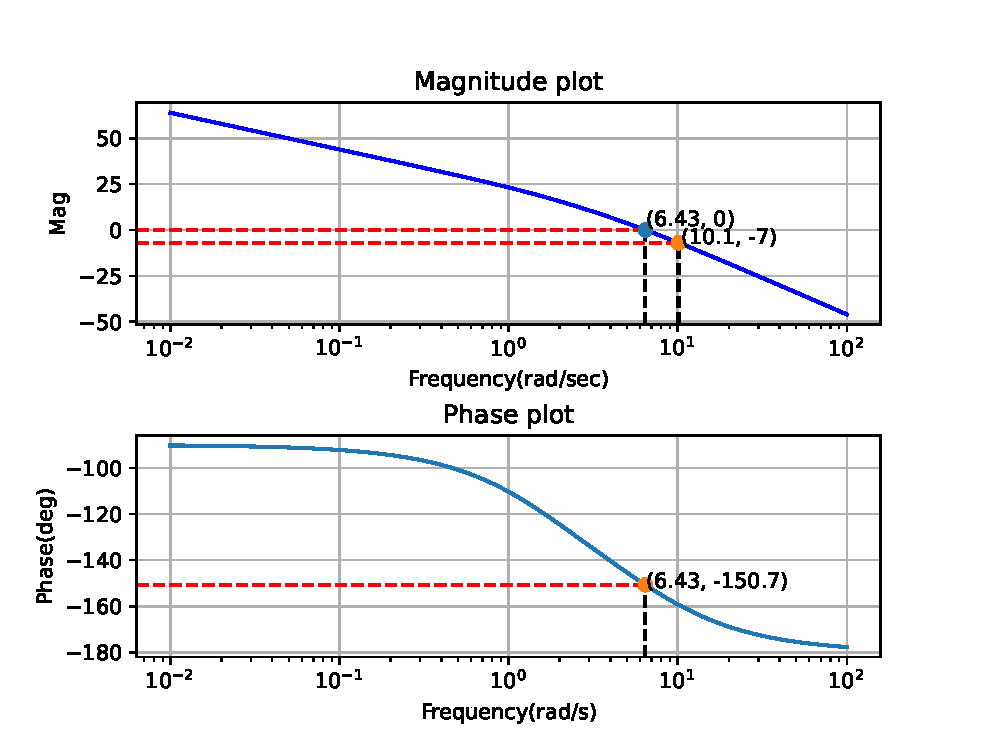
\includegraphics[width=\columnwidth]{./figs/ee18btech11047/ee18btech11047_2.eps}
\caption{1}
\label{fig:ee18btech11047_2}
\end{figure}
The phase margin is 
\begin{align}
\phi_{M} &= 180\degree-150.7\degree \implies \phi_{M} = 29.3\degree \label{eq:ee18btech11047_ph}
\end{align}
The closed-loop bandwith, $\omega_{BW}$(-3 dB frequency), equals the frequency at which the open-loop magnitude response is around -7 dB.
\begin{align}
\omega_{BW} = 10.1  rad/sec \label{eq:ee18btech11047_bw}
\end{align}
\textbf{Damping ratio:} \\
Substitute $\phi_{M}$ value from equation(\ref{eq:ee18btech11047_ph})
\begin{align}
\phi_{M} &= {tan}^{-1}\brak{\frac{2\zeta}{\sqrt{-2\zeta^{2}+\sqrt{1+4\zeta^{2}}}}}\\
\implies \zeta &= 0.34
\end{align}
\textbf{Settling time:} \\
Substitute $\omega_{BW}$ value from equation(\ref{eq:ee18btech11047_bw}) and $\zeta$
\begin{align}
T_{s}&= \frac{4}{\omega_{BW}\zeta}\sqrt{(1-2\zeta^2)+\sqrt{4\zeta^4-4\zeta^2+2}}\\
\implies T_{s} &= 1.65 sec   \\
\end{align}
\textbf{Peak time:}
\begin{align}
T_{p} &= \frac{\pi\zeta T_{s}}{4\sqrt{1-\zeta^2}}\\
\implies T_{p} &= 0.325 sec
\end{align}
\textbf{Percent overshoot:}
\begin{align}
\% OS&=100e^{-(\frac{\zeta\pi}{\sqrt{1-\zeta^2}})}\\
\implies \% OS &= 35.1 \%
\end{align}
Note that the answers will be approximate due to the dominant pole approximation.\\
The following code generates the step response of the system.
\begin{lstlisting}
codes/ee18btech11047/ee18btech11047_3.py
\end{lstlisting}
\begin{figure}[!ht]
\centering
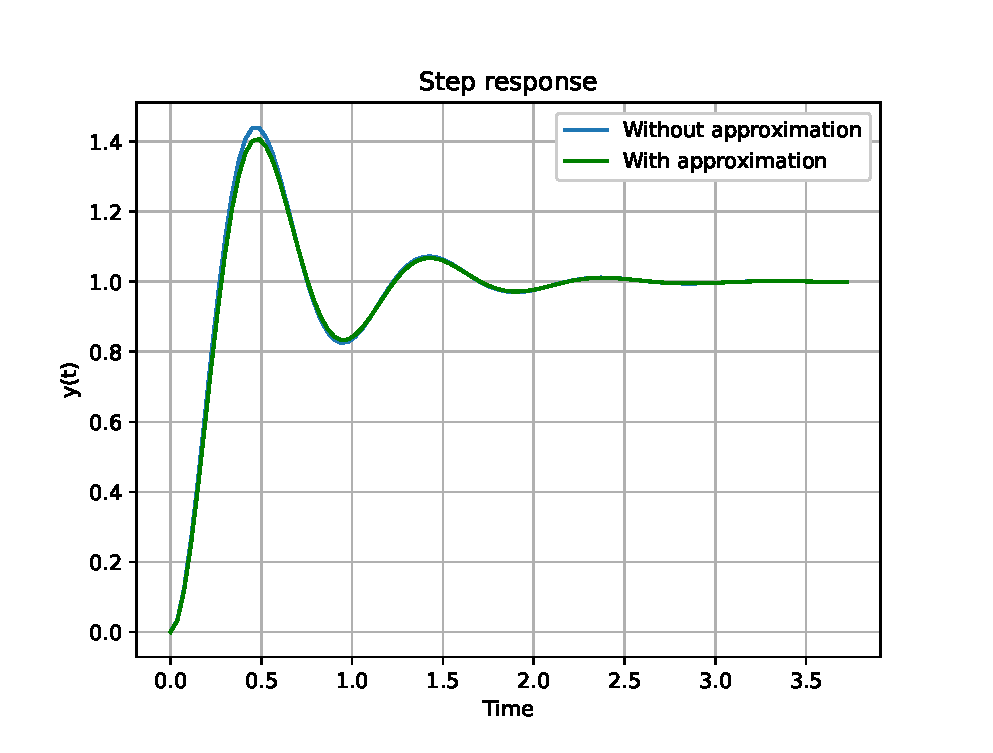
\includegraphics[width=\columnwidth]{./figs/ee18btech11047/ee18btech11047_3.eps}
\caption{2}
\label{fig:ee18btech11047_3}
\end{figure}
\item Find the approximate transfer function for the open loop transfer function
\begin{align}
G(s) &= \frac{75(1+0.2s)}{s(s^{2}+16s+100)}
\end{align}
\solution Using equation \eqref{eq:ee18btech11047_ctf}
\begin{align}
T(s) = \frac{75(1+0.2s)}{s^3 + 16s^2 + 115s +75} 
\end{align}
The following code gives the poles and zeros of the transfer function.
\begin{lstlisting}
codes/ee18btech11047/ee18btech11047_4.py
\end{lstlisting}
\begin{table}[!ht]
\centering
\input{./tables/ee18btech11047/ee18btech11047_2.tex}
\caption{}
\label{table:ee18btech11047_2}
\end{table}
The real part of the complex conjugate poles is comparable with the zero $z_{1}$ of the transfer function.So,they cancel out each other.
The approximated transfer function is of first order.
\begin{align}
T_{2}(s) &= \frac{K_{2}}{(s-p_{1})}\\
T(0) &= T_{2}(s)\\
\implies K_{2} &= p_{1} \\
T_{2}(s) &= \frac{0.72}{s+0.72}
\end{align}
\item Estimate the transient response of the obtained first order system.\\
\solution\\
\textbf{Time constant:}\\
The time constant is the time taken by the step response to rise to 63\% of it's final value.
\begin{align}
T &= \frac{1}{|pole|}\\
T &= \frac{1}{0.72} = 1.388 sec
\end{align}
\textbf{Rise time:}\\
Rise time is the time for the waveform to go from 0.1 to 0.9 of it's final value.
\begin{align}
T_{r} &= \frac{2.2}{|pole|}\\
T_{r} &= \frac{2.2}{0.72} = 3.05 sec
\end{align}
\textbf{Settling time:}\\
Settling time is defined as the time for the response to reach and stay within, 2\% of its final value.
\begin{align}
T_{s} &= \frac{4}{|pole|}\\
T_{s} &= \frac{4}{0.72}=5.55 sec
\end{align}
The following code plots the step response of the system.
\begin{lstlisting}
codes/ee18btech11047/ee18btech11047_5.py
\end{lstlisting}
\begin{figure}[!ht]
\centering
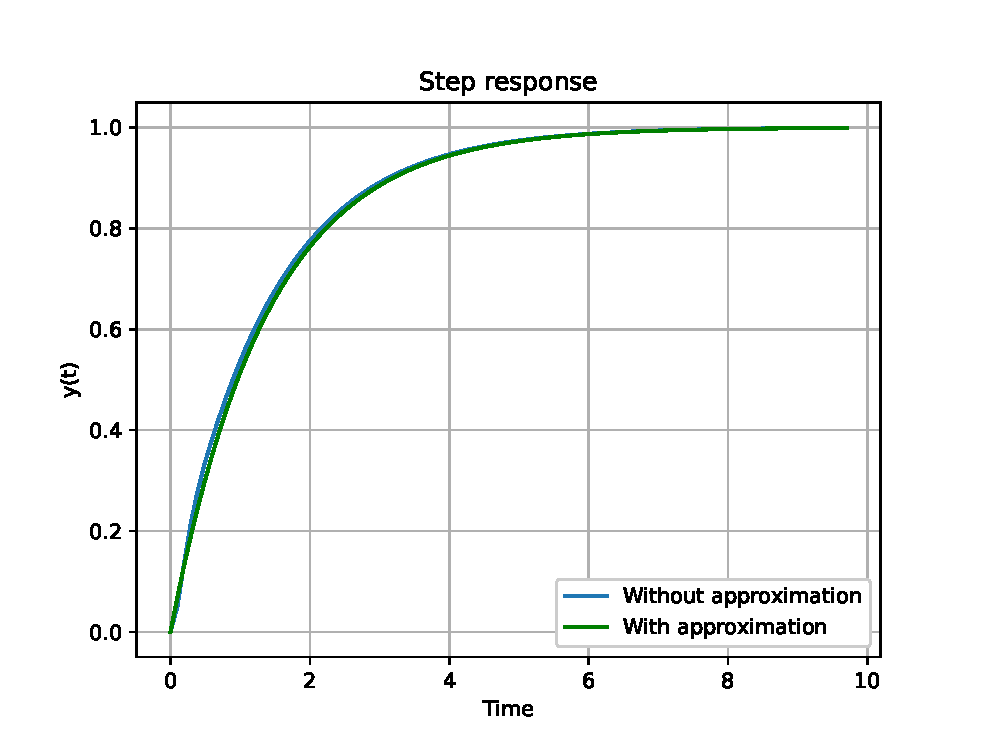
\includegraphics[width=\columnwidth]{./figs/ee18btech11047/ee18btech11047_4.eps}
\caption{}
\label{fig:ee18btech11047_4}
\end{figure}
\end{enumerate}
}
	\end{center}
\caption{}
\label{fig:ee18btech11047}
\end{figure}

\item Find the approximate transfer function for the open loop transfer function.
\begin{align}
G(s) &= \frac{50(s+3)(s+5)}{s(s+2)(s+4)(s+6)}
\end{align}
\solution Using equation\eqref{eq:ee18btech11047_ctf}
\begin{align}
T(s) &= \frac{50(s^{2}+8s+15)}{s^4+12s^3+94s^2+448s+750}
\end{align}
The following code gives the poles and zeros of the transfer function.
\begin{lstlisting}
codes/ee18btech11047/ee18btech11047_1.py
\end{lstlisting}
\begin{table}[!ht]
\centering
\begin{enumerate}[label=\thesubsection.\arabic*.,ref=\thesubsection.\theenumi]
\numberwithin{equation}{enumi}

\item Consider the following transfer functions as open-loop transfer functions in two different unity feedback(negative) systems.
\begin{align}
G(s) &= \frac{50(s+3)(s+5)}{s(s+2)(s+4)(s+6)} 
\\
G(s) &= \frac{75(1+0.2s)}{s(s^{2}+16s+100)} 
\end{align}
Estimate transient response of these systems from their respective bode plots.
\\
\solution 
\begin{enumerate}
\item  The dominant pole approximation is used to characterize higher order systems because it is difficult to characterize and analyse systems with order greater than 3.
\item Consider a transfer function.
\begin{align}
H(s) = K\frac{\alpha\beta}{(s+\alpha)(s+\beta)}
\end{align}
It has two poles $-\alpha$ and $-\beta $. If the magnitude of $\beta$ is very large compared to $\alpha$ (typically if $\frac{|\beta|}{|\alpha|}$ $>$ 5  ) we can approximate for the transfer function assuming $s$ is sufficiently small compared to $\beta$ as follows.
\begin{align}
H(s) = K_{2}\brak{\frac{1}{s+\alpha}}
\end{align}
Note that the value of $H(0)$ should be unchanged for the exact and approximate transfer functions.This is necessary to ensure that the final value of the step response is unchanged.
\begin{align}
\lim_{t\to\infty} y(t) &= \lim_{s\to 0} sY(s) \\
\lim_{t\to\infty} y(t) &= \lim_{s\to 0} sU(s)H(s) = H(0)
\end{align}
In order to acheive this we adjust the gain value of the approximated transfer function by equating $H(0)$ values.
\begin{align}
\implies H(s) = K\frac{\alpha}{(s+\alpha)}
\end{align}
\item In terms of poles, the pole closer to the origin is considered as the dominating pole.As considered above,the magnitude of $\alpha$ is small therefore the time constant $\frac{1}{\alpha}$ will be high and reaches equilibrium slowly and vice versa in case of  $\beta$.Therefore,this approximation assumes that the slowest part of the system dominates the response.The faster parts of the system are ignored.
\item Complex poles along with real poles : In this case the dominant pole(s) can be determined by comparing only the real parts.If the real part of the complex conjugate poles is greater in magnitude than the real pole, the two complex conjugate poles the dominant poles.
\item If the transfer function has zeros along with poles,we have to consider the fact that pole and zero cancel out each other if their respective magnitudes are comparable.
\end{enumerate}
\item Find the closed loop transfer function of a negative unity feedback system given open loop transfer function $G(s)$ .\\
\solution 
\begin{align}
\label{eq:ee18btech11047_ctf}
T(s) &= \frac{G(s)}{1+G(s)}
\end{align}
\begin{figure}[!ht]
	\begin{center}
		\resizebox{\columnwidth}{!}{\input{./figs/ee18btech11047/ee18btech11047.tex}}
	\end{center}
\caption{}
\label{fig:ee18btech11047}
\end{figure}

\item Find the approximate transfer function for the open loop transfer function.
\begin{align}
G(s) &= \frac{50(s+3)(s+5)}{s(s+2)(s+4)(s+6)}
\end{align}
\solution Using equation\eqref{eq:ee18btech11047_ctf}
\begin{align}
T(s) &= \frac{50(s^{2}+8s+15)}{s^4+12s^3+94s^2+448s+750}
\end{align}
The following code gives the poles and zeros of the transfer function.
\begin{lstlisting}
codes/ee18btech11047/ee18btech11047_1.py
\end{lstlisting}
\begin{table}[!ht]
\centering
\input{./tables/ee18btech11047/ee18btech11047.tex}
\caption{}
\label{table:ee18btech11047}
\end{table}
The real poles \brak{p_{1},p_{2}} and zeros \brak{z_{1},z_{2}} cancel out each other as mentioned above.So, we are left with the two conjugate poles.\\
The approximated transfer function is 
\begin{align}
T_{1}(s) &= \frac{K_{1}}{(s-p_{3})(s-p_{4})}\\ 
T(0) &= T_{1}(0)\\
\implies K_{1} &= p_{3}p_{4}\\
T_{1}(s) &= \frac{47.09}{s^{2}+3.74s+47.09}
\end{align}
\item Estimate the transient response of the obtained second order system using the respective bode plot.\\
\solution The following code generates the bode plot for open loop transfer function.
\begin{lstlisting}
codes/ee18btech11047/ee18btech11047_2.py
\end{lstlisting}
\begin{figure}[!ht]
\centering
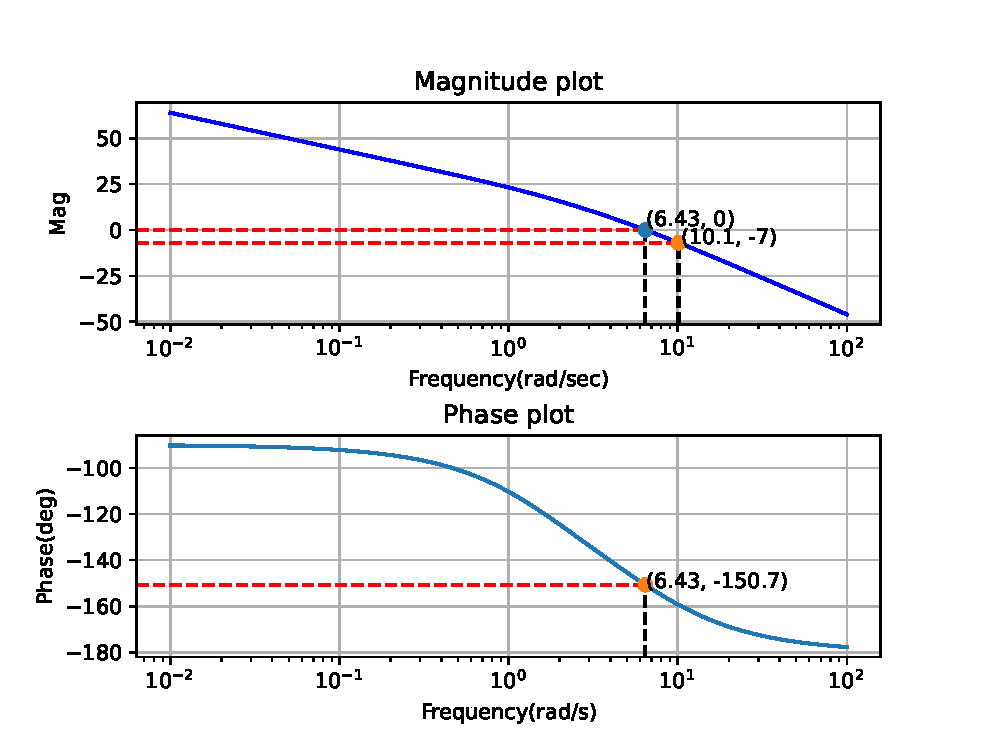
\includegraphics[width=\columnwidth]{./figs/ee18btech11047/ee18btech11047_2.eps}
\caption{1}
\label{fig:ee18btech11047_2}
\end{figure}
The phase margin is 
\begin{align}
\phi_{M} &= 180\degree-150.7\degree \implies \phi_{M} = 29.3\degree \label{eq:ee18btech11047_ph}
\end{align}
The closed-loop bandwith, $\omega_{BW}$(-3 dB frequency), equals the frequency at which the open-loop magnitude response is around -7 dB.
\begin{align}
\omega_{BW} = 10.1  rad/sec \label{eq:ee18btech11047_bw}
\end{align}
\textbf{Damping ratio:} \\
Substitute $\phi_{M}$ value from equation(\ref{eq:ee18btech11047_ph})
\begin{align}
\phi_{M} &= {tan}^{-1}\brak{\frac{2\zeta}{\sqrt{-2\zeta^{2}+\sqrt{1+4\zeta^{2}}}}}\\
\implies \zeta &= 0.34
\end{align}
\textbf{Settling time:} \\
Substitute $\omega_{BW}$ value from equation(\ref{eq:ee18btech11047_bw}) and $\zeta$
\begin{align}
T_{s}&= \frac{4}{\omega_{BW}\zeta}\sqrt{(1-2\zeta^2)+\sqrt{4\zeta^4-4\zeta^2+2}}\\
\implies T_{s} &= 1.65 sec   \\
\end{align}
\textbf{Peak time:}
\begin{align}
T_{p} &= \frac{\pi\zeta T_{s}}{4\sqrt{1-\zeta^2}}\\
\implies T_{p} &= 0.325 sec
\end{align}
\textbf{Percent overshoot:}
\begin{align}
\% OS&=100e^{-(\frac{\zeta\pi}{\sqrt{1-\zeta^2}})}\\
\implies \% OS &= 35.1 \%
\end{align}
Note that the answers will be approximate due to the dominant pole approximation.\\
The following code generates the step response of the system.
\begin{lstlisting}
codes/ee18btech11047/ee18btech11047_3.py
\end{lstlisting}
\begin{figure}[!ht]
\centering
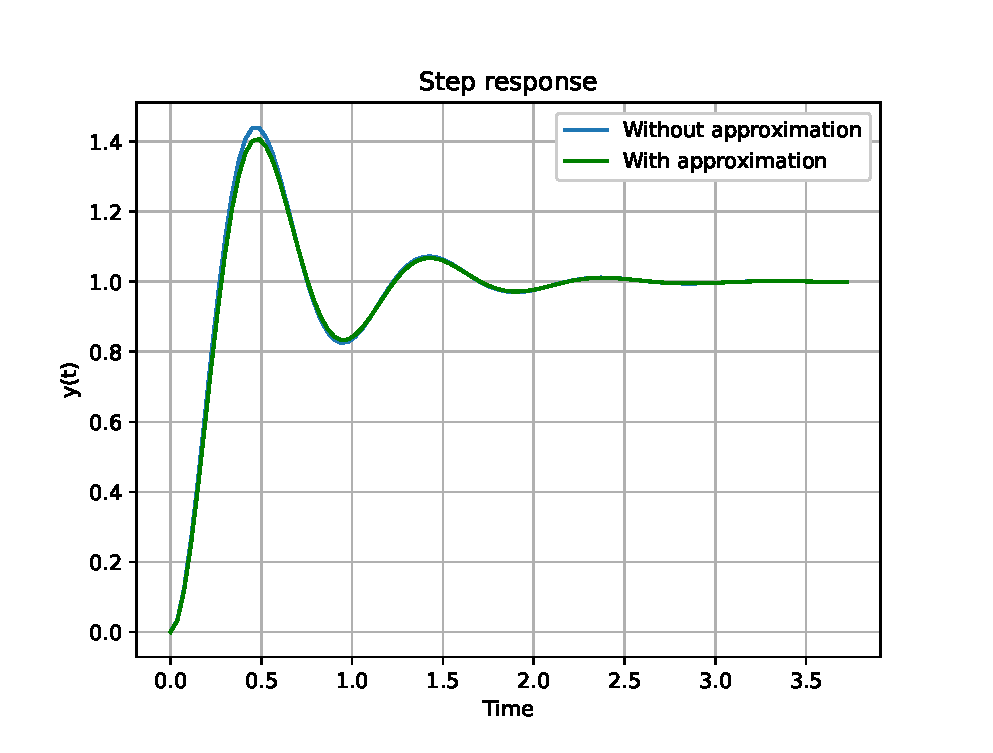
\includegraphics[width=\columnwidth]{./figs/ee18btech11047/ee18btech11047_3.eps}
\caption{2}
\label{fig:ee18btech11047_3}
\end{figure}
\item Find the approximate transfer function for the open loop transfer function
\begin{align}
G(s) &= \frac{75(1+0.2s)}{s(s^{2}+16s+100)}
\end{align}
\solution Using equation \eqref{eq:ee18btech11047_ctf}
\begin{align}
T(s) = \frac{75(1+0.2s)}{s^3 + 16s^2 + 115s +75} 
\end{align}
The following code gives the poles and zeros of the transfer function.
\begin{lstlisting}
codes/ee18btech11047/ee18btech11047_4.py
\end{lstlisting}
\begin{table}[!ht]
\centering
\input{./tables/ee18btech11047/ee18btech11047_2.tex}
\caption{}
\label{table:ee18btech11047_2}
\end{table}
The real part of the complex conjugate poles is comparable with the zero $z_{1}$ of the transfer function.So,they cancel out each other.
The approximated transfer function is of first order.
\begin{align}
T_{2}(s) &= \frac{K_{2}}{(s-p_{1})}\\
T(0) &= T_{2}(s)\\
\implies K_{2} &= p_{1} \\
T_{2}(s) &= \frac{0.72}{s+0.72}
\end{align}
\item Estimate the transient response of the obtained first order system.\\
\solution\\
\textbf{Time constant:}\\
The time constant is the time taken by the step response to rise to 63\% of it's final value.
\begin{align}
T &= \frac{1}{|pole|}\\
T &= \frac{1}{0.72} = 1.388 sec
\end{align}
\textbf{Rise time:}\\
Rise time is the time for the waveform to go from 0.1 to 0.9 of it's final value.
\begin{align}
T_{r} &= \frac{2.2}{|pole|}\\
T_{r} &= \frac{2.2}{0.72} = 3.05 sec
\end{align}
\textbf{Settling time:}\\
Settling time is defined as the time for the response to reach and stay within, 2\% of its final value.
\begin{align}
T_{s} &= \frac{4}{|pole|}\\
T_{s} &= \frac{4}{0.72}=5.55 sec
\end{align}
The following code plots the step response of the system.
\begin{lstlisting}
codes/ee18btech11047/ee18btech11047_5.py
\end{lstlisting}
\begin{figure}[!ht]
\centering
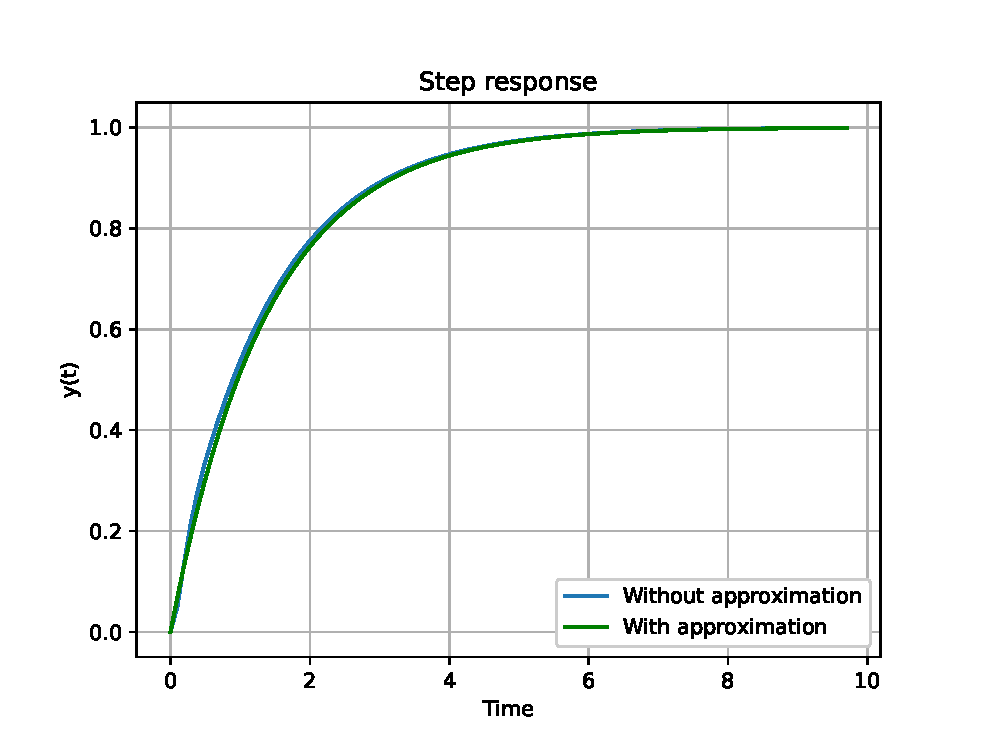
\includegraphics[width=\columnwidth]{./figs/ee18btech11047/ee18btech11047_4.eps}
\caption{}
\label{fig:ee18btech11047_4}
\end{figure}
\end{enumerate}

\caption{}
\label{table:ee18btech11047}
\end{table}
The real poles \brak{p_{1},p_{2}} and zeros \brak{z_{1},z_{2}} cancel out each other as mentioned above.So, we are left with the two conjugate poles.\\
The approximated transfer function is 
\begin{align}
T_{1}(s) &= \frac{K_{1}}{(s-p_{3})(s-p_{4})}\\ 
T(0) &= T_{1}(0)\\
\implies K_{1} &= p_{3}p_{4}\\
T_{1}(s) &= \frac{47.09}{s^{2}+3.74s+47.09}
\end{align}
\item Estimate the transient response of the obtained second order system using the respective bode plot.\\
\solution The following code generates the bode plot for open loop transfer function.
\begin{lstlisting}
codes/ee18btech11047/ee18btech11047_2.py
\end{lstlisting}
\begin{figure}[!ht]
\centering
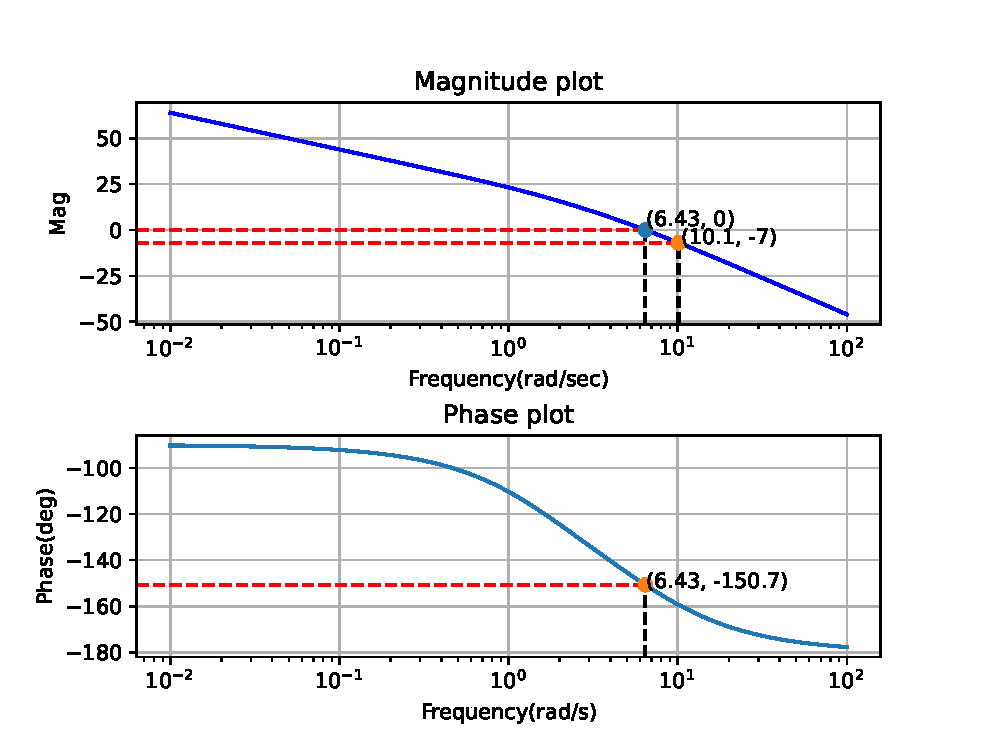
\includegraphics[width=\columnwidth]{./figs/ee18btech11047/ee18btech11047_2.eps}
\caption{1}
\label{fig:ee18btech11047_2}
\end{figure}
The phase margin is 
\begin{align}
\phi_{M} &= 180\degree-150.7\degree \implies \phi_{M} = 29.3\degree \label{eq:ee18btech11047_ph}
\end{align}
The closed-loop bandwith, $\omega_{BW}$(-3 dB frequency), equals the frequency at which the open-loop magnitude response is around -7 dB.
\begin{align}
\omega_{BW} = 10.1  rad/sec \label{eq:ee18btech11047_bw}
\end{align}
\textbf{Damping ratio:} \\
Substitute $\phi_{M}$ value from equation(\ref{eq:ee18btech11047_ph})
\begin{align}
\phi_{M} &= {tan}^{-1}\brak{\frac{2\zeta}{\sqrt{-2\zeta^{2}+\sqrt{1+4\zeta^{2}}}}}\\
\implies \zeta &= 0.34
\end{align}
\textbf{Settling time:} \\
Substitute $\omega_{BW}$ value from equation(\ref{eq:ee18btech11047_bw}) and $\zeta$
\begin{align}
T_{s}&= \frac{4}{\omega_{BW}\zeta}\sqrt{(1-2\zeta^2)+\sqrt{4\zeta^4-4\zeta^2+2}}\\
\implies T_{s} &= 1.65 sec   \\
\end{align}
\textbf{Peak time:}
\begin{align}
T_{p} &= \frac{\pi\zeta T_{s}}{4\sqrt{1-\zeta^2}}\\
\implies T_{p} &= 0.325 sec
\end{align}
\textbf{Percent overshoot:}
\begin{align}
\% OS&=100e^{-(\frac{\zeta\pi}{\sqrt{1-\zeta^2}})}\\
\implies \% OS &= 35.1 \%
\end{align}
Note that the answers will be approximate due to the dominant pole approximation.\\
The following code generates the step response of the system.
\begin{lstlisting}
codes/ee18btech11047/ee18btech11047_3.py
\end{lstlisting}
\begin{figure}[!ht]
\centering
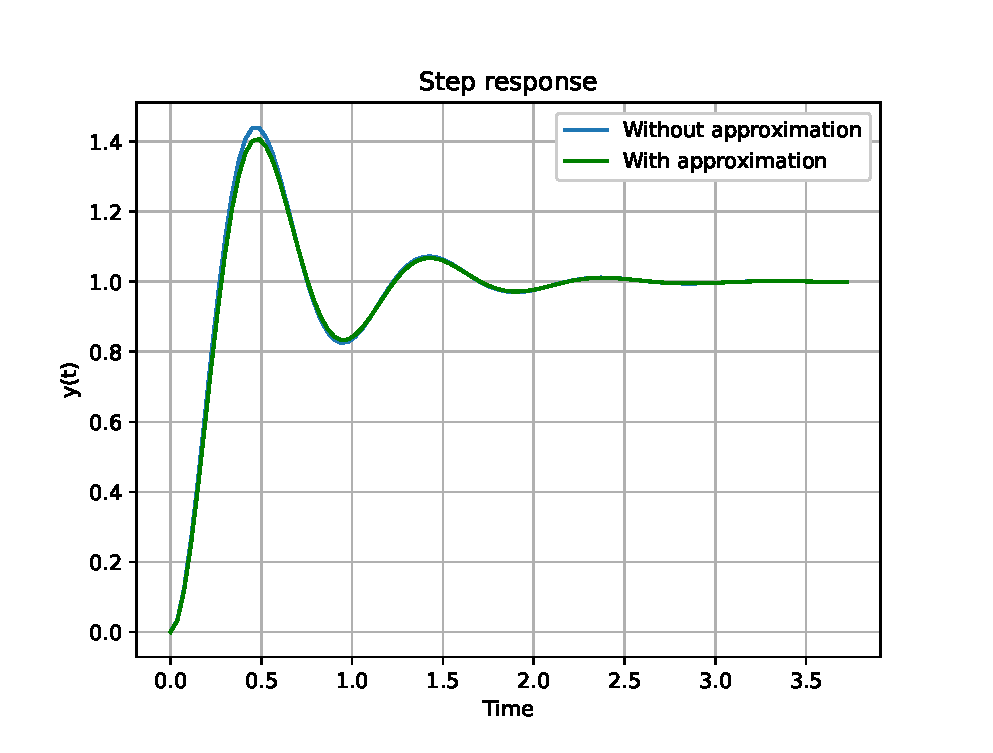
\includegraphics[width=\columnwidth]{./figs/ee18btech11047/ee18btech11047_3.eps}
\caption{2}
\label{fig:ee18btech11047_3}
\end{figure}
\item Find the approximate transfer function for the open loop transfer function
\begin{align}
G(s) &= \frac{75(1+0.2s)}{s(s^{2}+16s+100)}
\end{align}
\solution Using equation \eqref{eq:ee18btech11047_ctf}
\begin{align}
T(s) = \frac{75(1+0.2s)}{s^3 + 16s^2 + 115s +75} 
\end{align}
The following code gives the poles and zeros of the transfer function.
\begin{lstlisting}
codes/ee18btech11047/ee18btech11047_4.py
\end{lstlisting}
\begin{table}[!ht]
\centering
\tikzstyle{block} = [draw, fill=blue!20, rectangle, 
    minimum height=3em, minimum width=6em]
\tikzstyle{sum} = [draw, fill=blue!20, circle, node distance=1cm]
\tikzstyle{input} = [coordinate]
\tikzstyle{output} = [coordinate]
\tikzstyle{pinstyle} = [pin edge={to-,thin,black}]

\begin{tikzpicture}[auto, node distance=2cm,>=latex']
    \node [input, name=input] {};
    \node [sum, right of=input] (sum) {};
    \node [block, right of=sum] (controller) {$G$};
    \node [output, right of=controller] (output) {};
    \node [block, below of=controller] (feedback) {$H$};
    \draw [draw,->] (input) -- node {} (sum);
    \draw [->] (sum) -- node {$V_i$} (controller);
    \draw [->] (controller) -- node [name=y] {$V_o$}(output);
    \draw [->] (y) |- (feedback);
    \draw [->] (feedback) -| node[pos=0.99]{$+$}  node [near end] {$V_f$} (sum);
\end{tikzpicture}

\caption{}
\label{table:ee18btech11047_2}
\end{table}
The real part of the complex conjugate poles is comparable with the zero $z_{1}$ of the transfer function.So,they cancel out each other.
The approximated transfer function is of first order.
\begin{align}
T_{2}(s) &= \frac{K_{2}}{(s-p_{1})}\\
T(0) &= T_{2}(s)\\
\implies K_{2} &= p_{1} \\
T_{2}(s) &= \frac{0.72}{s+0.72}
\end{align}
\item Estimate the transient response of the obtained first order system.\\
\solution\\
\textbf{Time constant:}\\
The time constant is the time taken by the step response to rise to 63\% of it's final value.
\begin{align}
T &= \frac{1}{|pole|}\\
T &= \frac{1}{0.72} = 1.388 sec
\end{align}
\textbf{Rise time:}\\
Rise time is the time for the waveform to go from 0.1 to 0.9 of it's final value.
\begin{align}
T_{r} &= \frac{2.2}{|pole|}\\
T_{r} &= \frac{2.2}{0.72} = 3.05 sec
\end{align}
\textbf{Settling time:}\\
Settling time is defined as the time for the response to reach and stay within, 2\% of its final value.
\begin{align}
T_{s} &= \frac{4}{|pole|}\\
T_{s} &= \frac{4}{0.72}=5.55 sec
\end{align}
The following code plots the step response of the system.
\begin{lstlisting}
codes/ee18btech11047/ee18btech11047_5.py
\end{lstlisting}
\begin{figure}[!ht]
\centering
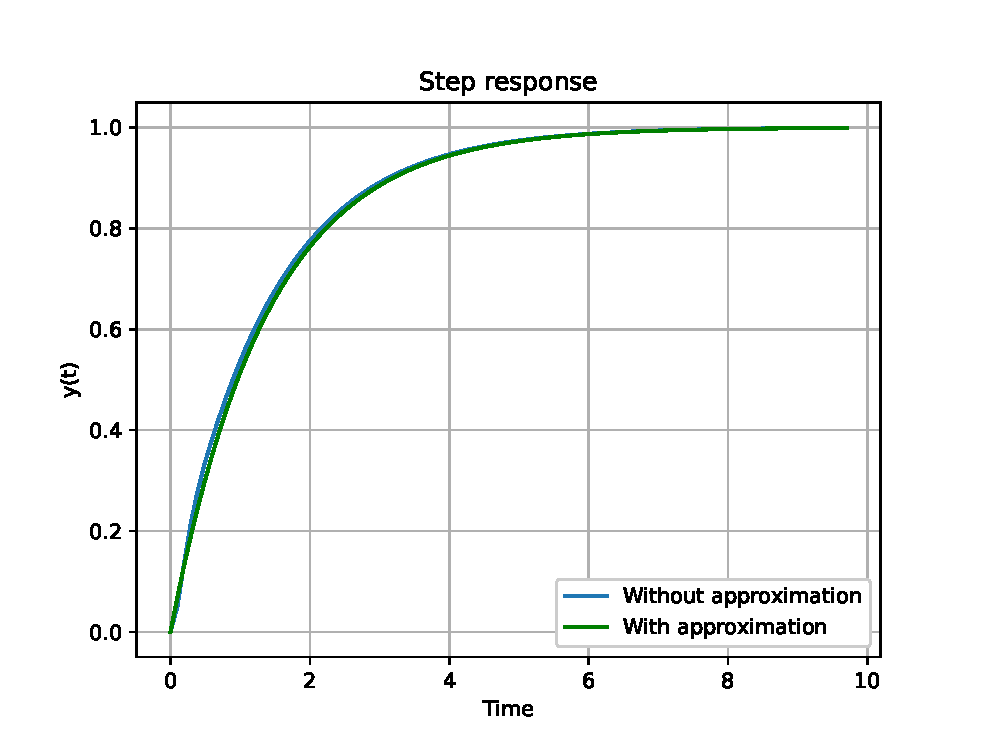
\includegraphics[width=\columnwidth]{./figs/ee18btech11047/ee18btech11047_4.eps}
\caption{}
\label{fig:ee18btech11047_4}
\end{figure}
\end{enumerate}
}
	\end{center}
\caption{}
\label{fig:ee18btech11047}
\end{figure}

\item Find the approximate transfer function for the open loop transfer function.
\begin{align}
G(s) &= \frac{50(s+3)(s+5)}{s(s+2)(s+4)(s+6)}
\end{align}
\solution Using equation\eqref{eq:ee18btech11047_ctf}
\begin{align}
T(s) &= \frac{50(s^{2}+8s+15)}{s^4+12s^3+94s^2+448s+750}
\end{align}
The following code gives the poles and zeros of the transfer function.
\begin{lstlisting}
codes/ee18btech11047/ee18btech11047_1.py
\end{lstlisting}
\begin{table}[!ht]
\centering
\begin{enumerate}[label=\thesubsection.\arabic*.,ref=\thesubsection.\theenumi]
\numberwithin{equation}{enumi}

\item Consider the following transfer functions as open-loop transfer functions in two different unity feedback(negative) systems.
\begin{align}
G(s) &= \frac{50(s+3)(s+5)}{s(s+2)(s+4)(s+6)} 
\\
G(s) &= \frac{75(1+0.2s)}{s(s^{2}+16s+100)} 
\end{align}
Estimate transient response of these systems from their respective bode plots.
\\
\solution 
\begin{enumerate}
\item  The dominant pole approximation is used to characterize higher order systems because it is difficult to characterize and analyse systems with order greater than 3.
\item Consider a transfer function.
\begin{align}
H(s) = K\frac{\alpha\beta}{(s+\alpha)(s+\beta)}
\end{align}
It has two poles $-\alpha$ and $-\beta $. If the magnitude of $\beta$ is very large compared to $\alpha$ (typically if $\frac{|\beta|}{|\alpha|}$ $>$ 5  ) we can approximate for the transfer function assuming $s$ is sufficiently small compared to $\beta$ as follows.
\begin{align}
H(s) = K_{2}\brak{\frac{1}{s+\alpha}}
\end{align}
Note that the value of $H(0)$ should be unchanged for the exact and approximate transfer functions.This is necessary to ensure that the final value of the step response is unchanged.
\begin{align}
\lim_{t\to\infty} y(t) &= \lim_{s\to 0} sY(s) \\
\lim_{t\to\infty} y(t) &= \lim_{s\to 0} sU(s)H(s) = H(0)
\end{align}
In order to acheive this we adjust the gain value of the approximated transfer function by equating $H(0)$ values.
\begin{align}
\implies H(s) = K\frac{\alpha}{(s+\alpha)}
\end{align}
\item In terms of poles, the pole closer to the origin is considered as the dominating pole.As considered above,the magnitude of $\alpha$ is small therefore the time constant $\frac{1}{\alpha}$ will be high and reaches equilibrium slowly and vice versa in case of  $\beta$.Therefore,this approximation assumes that the slowest part of the system dominates the response.The faster parts of the system are ignored.
\item Complex poles along with real poles : In this case the dominant pole(s) can be determined by comparing only the real parts.If the real part of the complex conjugate poles is greater in magnitude than the real pole, the two complex conjugate poles the dominant poles.
\item If the transfer function has zeros along with poles,we have to consider the fact that pole and zero cancel out each other if their respective magnitudes are comparable.
\end{enumerate}
\item Find the closed loop transfer function of a negative unity feedback system given open loop transfer function $G(s)$ .\\
\solution 
\begin{align}
\label{eq:ee18btech11047_ctf}
T(s) &= \frac{G(s)}{1+G(s)}
\end{align}
\begin{figure}[!ht]
	\begin{center}
		\resizebox{\columnwidth}{!}{\begin{enumerate}[label=\thesubsection.\arabic*.,ref=\thesubsection.\theenumi]
\numberwithin{equation}{enumi}

\item Consider the following transfer functions as open-loop transfer functions in two different unity feedback(negative) systems.
\begin{align}
G(s) &= \frac{50(s+3)(s+5)}{s(s+2)(s+4)(s+6)} 
\\
G(s) &= \frac{75(1+0.2s)}{s(s^{2}+16s+100)} 
\end{align}
Estimate transient response of these systems from their respective bode plots.
\\
\solution 
\begin{enumerate}
\item  The dominant pole approximation is used to characterize higher order systems because it is difficult to characterize and analyse systems with order greater than 3.
\item Consider a transfer function.
\begin{align}
H(s) = K\frac{\alpha\beta}{(s+\alpha)(s+\beta)}
\end{align}
It has two poles $-\alpha$ and $-\beta $. If the magnitude of $\beta$ is very large compared to $\alpha$ (typically if $\frac{|\beta|}{|\alpha|}$ $>$ 5  ) we can approximate for the transfer function assuming $s$ is sufficiently small compared to $\beta$ as follows.
\begin{align}
H(s) = K_{2}\brak{\frac{1}{s+\alpha}}
\end{align}
Note that the value of $H(0)$ should be unchanged for the exact and approximate transfer functions.This is necessary to ensure that the final value of the step response is unchanged.
\begin{align}
\lim_{t\to\infty} y(t) &= \lim_{s\to 0} sY(s) \\
\lim_{t\to\infty} y(t) &= \lim_{s\to 0} sU(s)H(s) = H(0)
\end{align}
In order to acheive this we adjust the gain value of the approximated transfer function by equating $H(0)$ values.
\begin{align}
\implies H(s) = K\frac{\alpha}{(s+\alpha)}
\end{align}
\item In terms of poles, the pole closer to the origin is considered as the dominating pole.As considered above,the magnitude of $\alpha$ is small therefore the time constant $\frac{1}{\alpha}$ will be high and reaches equilibrium slowly and vice versa in case of  $\beta$.Therefore,this approximation assumes that the slowest part of the system dominates the response.The faster parts of the system are ignored.
\item Complex poles along with real poles : In this case the dominant pole(s) can be determined by comparing only the real parts.If the real part of the complex conjugate poles is greater in magnitude than the real pole, the two complex conjugate poles the dominant poles.
\item If the transfer function has zeros along with poles,we have to consider the fact that pole and zero cancel out each other if their respective magnitudes are comparable.
\end{enumerate}
\item Find the closed loop transfer function of a negative unity feedback system given open loop transfer function $G(s)$ .\\
\solution 
\begin{align}
\label{eq:ee18btech11047_ctf}
T(s) &= \frac{G(s)}{1+G(s)}
\end{align}
\begin{figure}[!ht]
	\begin{center}
		\resizebox{\columnwidth}{!}{\input{./figs/ee18btech11047/ee18btech11047.tex}}
	\end{center}
\caption{}
\label{fig:ee18btech11047}
\end{figure}

\item Find the approximate transfer function for the open loop transfer function.
\begin{align}
G(s) &= \frac{50(s+3)(s+5)}{s(s+2)(s+4)(s+6)}
\end{align}
\solution Using equation\eqref{eq:ee18btech11047_ctf}
\begin{align}
T(s) &= \frac{50(s^{2}+8s+15)}{s^4+12s^3+94s^2+448s+750}
\end{align}
The following code gives the poles and zeros of the transfer function.
\begin{lstlisting}
codes/ee18btech11047/ee18btech11047_1.py
\end{lstlisting}
\begin{table}[!ht]
\centering
\input{./tables/ee18btech11047/ee18btech11047.tex}
\caption{}
\label{table:ee18btech11047}
\end{table}
The real poles \brak{p_{1},p_{2}} and zeros \brak{z_{1},z_{2}} cancel out each other as mentioned above.So, we are left with the two conjugate poles.\\
The approximated transfer function is 
\begin{align}
T_{1}(s) &= \frac{K_{1}}{(s-p_{3})(s-p_{4})}\\ 
T(0) &= T_{1}(0)\\
\implies K_{1} &= p_{3}p_{4}\\
T_{1}(s) &= \frac{47.09}{s^{2}+3.74s+47.09}
\end{align}
\item Estimate the transient response of the obtained second order system using the respective bode plot.\\
\solution The following code generates the bode plot for open loop transfer function.
\begin{lstlisting}
codes/ee18btech11047/ee18btech11047_2.py
\end{lstlisting}
\begin{figure}[!ht]
\centering
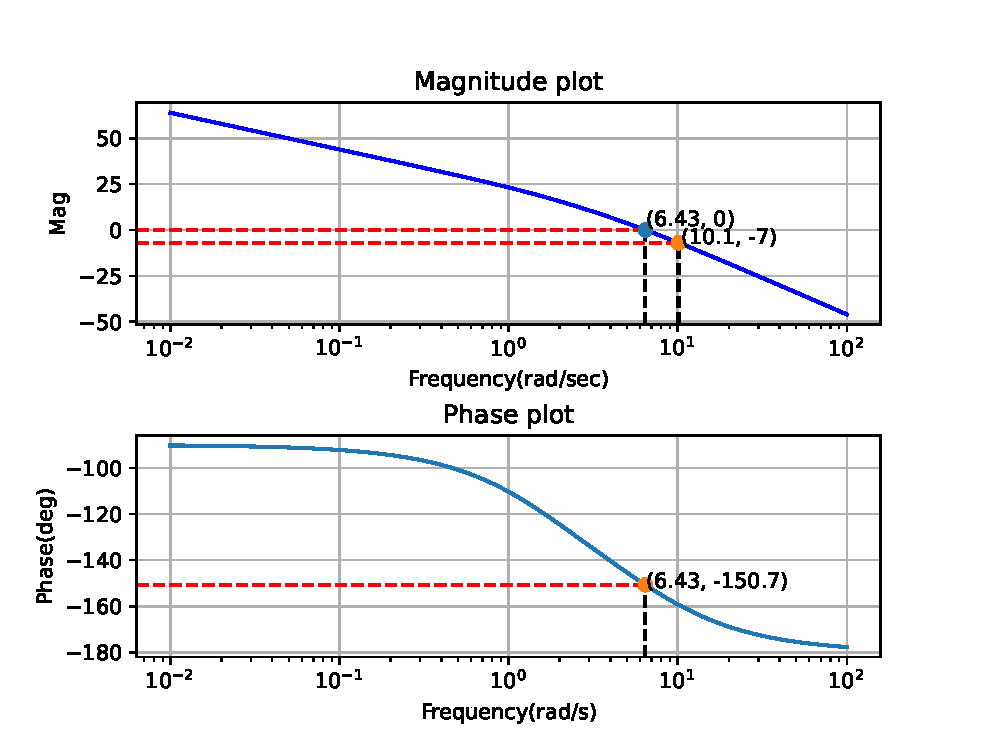
\includegraphics[width=\columnwidth]{./figs/ee18btech11047/ee18btech11047_2.eps}
\caption{1}
\label{fig:ee18btech11047_2}
\end{figure}
The phase margin is 
\begin{align}
\phi_{M} &= 180\degree-150.7\degree \implies \phi_{M} = 29.3\degree \label{eq:ee18btech11047_ph}
\end{align}
The closed-loop bandwith, $\omega_{BW}$(-3 dB frequency), equals the frequency at which the open-loop magnitude response is around -7 dB.
\begin{align}
\omega_{BW} = 10.1  rad/sec \label{eq:ee18btech11047_bw}
\end{align}
\textbf{Damping ratio:} \\
Substitute $\phi_{M}$ value from equation(\ref{eq:ee18btech11047_ph})
\begin{align}
\phi_{M} &= {tan}^{-1}\brak{\frac{2\zeta}{\sqrt{-2\zeta^{2}+\sqrt{1+4\zeta^{2}}}}}\\
\implies \zeta &= 0.34
\end{align}
\textbf{Settling time:} \\
Substitute $\omega_{BW}$ value from equation(\ref{eq:ee18btech11047_bw}) and $\zeta$
\begin{align}
T_{s}&= \frac{4}{\omega_{BW}\zeta}\sqrt{(1-2\zeta^2)+\sqrt{4\zeta^4-4\zeta^2+2}}\\
\implies T_{s} &= 1.65 sec   \\
\end{align}
\textbf{Peak time:}
\begin{align}
T_{p} &= \frac{\pi\zeta T_{s}}{4\sqrt{1-\zeta^2}}\\
\implies T_{p} &= 0.325 sec
\end{align}
\textbf{Percent overshoot:}
\begin{align}
\% OS&=100e^{-(\frac{\zeta\pi}{\sqrt{1-\zeta^2}})}\\
\implies \% OS &= 35.1 \%
\end{align}
Note that the answers will be approximate due to the dominant pole approximation.\\
The following code generates the step response of the system.
\begin{lstlisting}
codes/ee18btech11047/ee18btech11047_3.py
\end{lstlisting}
\begin{figure}[!ht]
\centering
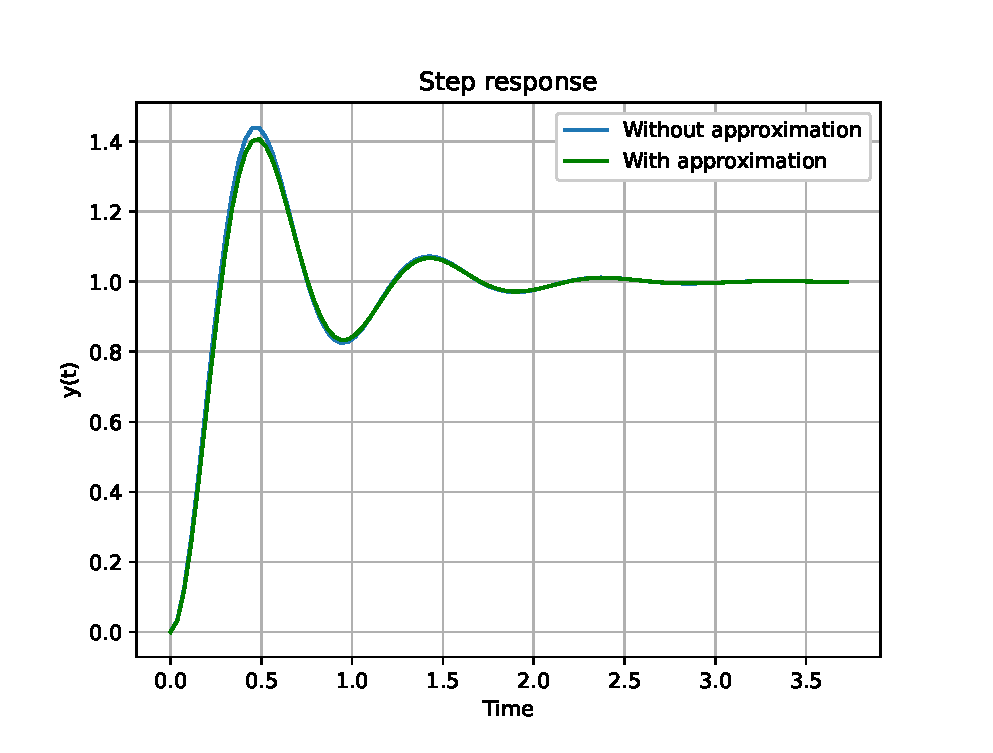
\includegraphics[width=\columnwidth]{./figs/ee18btech11047/ee18btech11047_3.eps}
\caption{2}
\label{fig:ee18btech11047_3}
\end{figure}
\item Find the approximate transfer function for the open loop transfer function
\begin{align}
G(s) &= \frac{75(1+0.2s)}{s(s^{2}+16s+100)}
\end{align}
\solution Using equation \eqref{eq:ee18btech11047_ctf}
\begin{align}
T(s) = \frac{75(1+0.2s)}{s^3 + 16s^2 + 115s +75} 
\end{align}
The following code gives the poles and zeros of the transfer function.
\begin{lstlisting}
codes/ee18btech11047/ee18btech11047_4.py
\end{lstlisting}
\begin{table}[!ht]
\centering
\input{./tables/ee18btech11047/ee18btech11047_2.tex}
\caption{}
\label{table:ee18btech11047_2}
\end{table}
The real part of the complex conjugate poles is comparable with the zero $z_{1}$ of the transfer function.So,they cancel out each other.
The approximated transfer function is of first order.
\begin{align}
T_{2}(s) &= \frac{K_{2}}{(s-p_{1})}\\
T(0) &= T_{2}(s)\\
\implies K_{2} &= p_{1} \\
T_{2}(s) &= \frac{0.72}{s+0.72}
\end{align}
\item Estimate the transient response of the obtained first order system.\\
\solution\\
\textbf{Time constant:}\\
The time constant is the time taken by the step response to rise to 63\% of it's final value.
\begin{align}
T &= \frac{1}{|pole|}\\
T &= \frac{1}{0.72} = 1.388 sec
\end{align}
\textbf{Rise time:}\\
Rise time is the time for the waveform to go from 0.1 to 0.9 of it's final value.
\begin{align}
T_{r} &= \frac{2.2}{|pole|}\\
T_{r} &= \frac{2.2}{0.72} = 3.05 sec
\end{align}
\textbf{Settling time:}\\
Settling time is defined as the time for the response to reach and stay within, 2\% of its final value.
\begin{align}
T_{s} &= \frac{4}{|pole|}\\
T_{s} &= \frac{4}{0.72}=5.55 sec
\end{align}
The following code plots the step response of the system.
\begin{lstlisting}
codes/ee18btech11047/ee18btech11047_5.py
\end{lstlisting}
\begin{figure}[!ht]
\centering
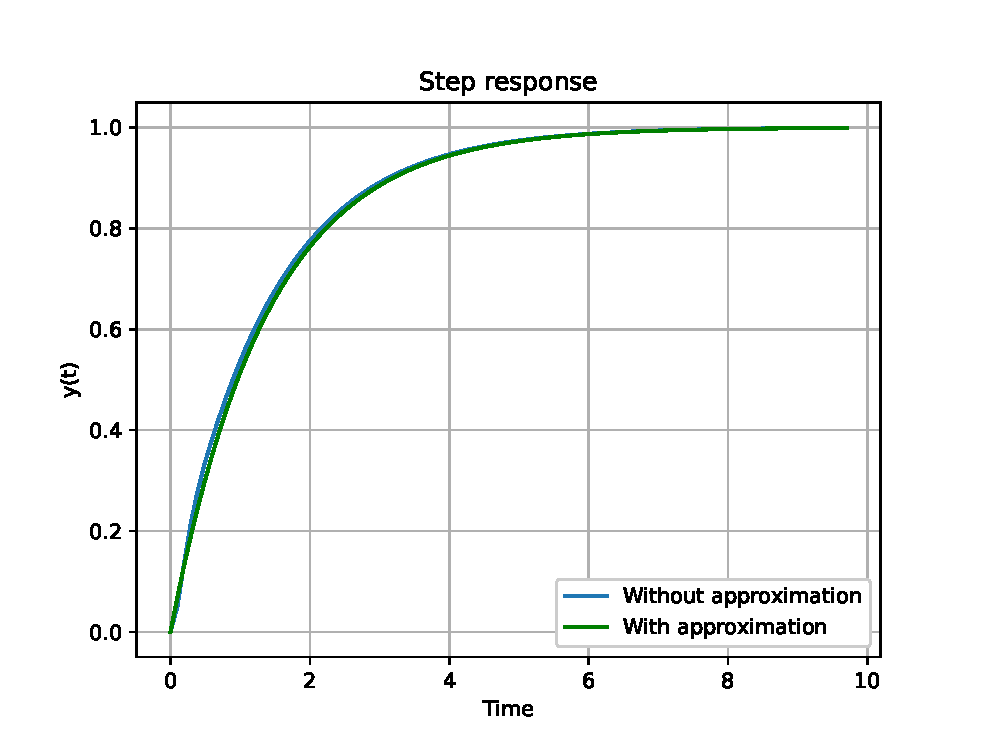
\includegraphics[width=\columnwidth]{./figs/ee18btech11047/ee18btech11047_4.eps}
\caption{}
\label{fig:ee18btech11047_4}
\end{figure}
\end{enumerate}
}
	\end{center}
\caption{}
\label{fig:ee18btech11047}
\end{figure}

\item Find the approximate transfer function for the open loop transfer function.
\begin{align}
G(s) &= \frac{50(s+3)(s+5)}{s(s+2)(s+4)(s+6)}
\end{align}
\solution Using equation\eqref{eq:ee18btech11047_ctf}
\begin{align}
T(s) &= \frac{50(s^{2}+8s+15)}{s^4+12s^3+94s^2+448s+750}
\end{align}
The following code gives the poles and zeros of the transfer function.
\begin{lstlisting}
codes/ee18btech11047/ee18btech11047_1.py
\end{lstlisting}
\begin{table}[!ht]
\centering
\begin{enumerate}[label=\thesubsection.\arabic*.,ref=\thesubsection.\theenumi]
\numberwithin{equation}{enumi}

\item Consider the following transfer functions as open-loop transfer functions in two different unity feedback(negative) systems.
\begin{align}
G(s) &= \frac{50(s+3)(s+5)}{s(s+2)(s+4)(s+6)} 
\\
G(s) &= \frac{75(1+0.2s)}{s(s^{2}+16s+100)} 
\end{align}
Estimate transient response of these systems from their respective bode plots.
\\
\solution 
\begin{enumerate}
\item  The dominant pole approximation is used to characterize higher order systems because it is difficult to characterize and analyse systems with order greater than 3.
\item Consider a transfer function.
\begin{align}
H(s) = K\frac{\alpha\beta}{(s+\alpha)(s+\beta)}
\end{align}
It has two poles $-\alpha$ and $-\beta $. If the magnitude of $\beta$ is very large compared to $\alpha$ (typically if $\frac{|\beta|}{|\alpha|}$ $>$ 5  ) we can approximate for the transfer function assuming $s$ is sufficiently small compared to $\beta$ as follows.
\begin{align}
H(s) = K_{2}\brak{\frac{1}{s+\alpha}}
\end{align}
Note that the value of $H(0)$ should be unchanged for the exact and approximate transfer functions.This is necessary to ensure that the final value of the step response is unchanged.
\begin{align}
\lim_{t\to\infty} y(t) &= \lim_{s\to 0} sY(s) \\
\lim_{t\to\infty} y(t) &= \lim_{s\to 0} sU(s)H(s) = H(0)
\end{align}
In order to acheive this we adjust the gain value of the approximated transfer function by equating $H(0)$ values.
\begin{align}
\implies H(s) = K\frac{\alpha}{(s+\alpha)}
\end{align}
\item In terms of poles, the pole closer to the origin is considered as the dominating pole.As considered above,the magnitude of $\alpha$ is small therefore the time constant $\frac{1}{\alpha}$ will be high and reaches equilibrium slowly and vice versa in case of  $\beta$.Therefore,this approximation assumes that the slowest part of the system dominates the response.The faster parts of the system are ignored.
\item Complex poles along with real poles : In this case the dominant pole(s) can be determined by comparing only the real parts.If the real part of the complex conjugate poles is greater in magnitude than the real pole, the two complex conjugate poles the dominant poles.
\item If the transfer function has zeros along with poles,we have to consider the fact that pole and zero cancel out each other if their respective magnitudes are comparable.
\end{enumerate}
\item Find the closed loop transfer function of a negative unity feedback system given open loop transfer function $G(s)$ .\\
\solution 
\begin{align}
\label{eq:ee18btech11047_ctf}
T(s) &= \frac{G(s)}{1+G(s)}
\end{align}
\begin{figure}[!ht]
	\begin{center}
		\resizebox{\columnwidth}{!}{\input{./figs/ee18btech11047/ee18btech11047.tex}}
	\end{center}
\caption{}
\label{fig:ee18btech11047}
\end{figure}

\item Find the approximate transfer function for the open loop transfer function.
\begin{align}
G(s) &= \frac{50(s+3)(s+5)}{s(s+2)(s+4)(s+6)}
\end{align}
\solution Using equation\eqref{eq:ee18btech11047_ctf}
\begin{align}
T(s) &= \frac{50(s^{2}+8s+15)}{s^4+12s^3+94s^2+448s+750}
\end{align}
The following code gives the poles and zeros of the transfer function.
\begin{lstlisting}
codes/ee18btech11047/ee18btech11047_1.py
\end{lstlisting}
\begin{table}[!ht]
\centering
\input{./tables/ee18btech11047/ee18btech11047.tex}
\caption{}
\label{table:ee18btech11047}
\end{table}
The real poles \brak{p_{1},p_{2}} and zeros \brak{z_{1},z_{2}} cancel out each other as mentioned above.So, we are left with the two conjugate poles.\\
The approximated transfer function is 
\begin{align}
T_{1}(s) &= \frac{K_{1}}{(s-p_{3})(s-p_{4})}\\ 
T(0) &= T_{1}(0)\\
\implies K_{1} &= p_{3}p_{4}\\
T_{1}(s) &= \frac{47.09}{s^{2}+3.74s+47.09}
\end{align}
\item Estimate the transient response of the obtained second order system using the respective bode plot.\\
\solution The following code generates the bode plot for open loop transfer function.
\begin{lstlisting}
codes/ee18btech11047/ee18btech11047_2.py
\end{lstlisting}
\begin{figure}[!ht]
\centering
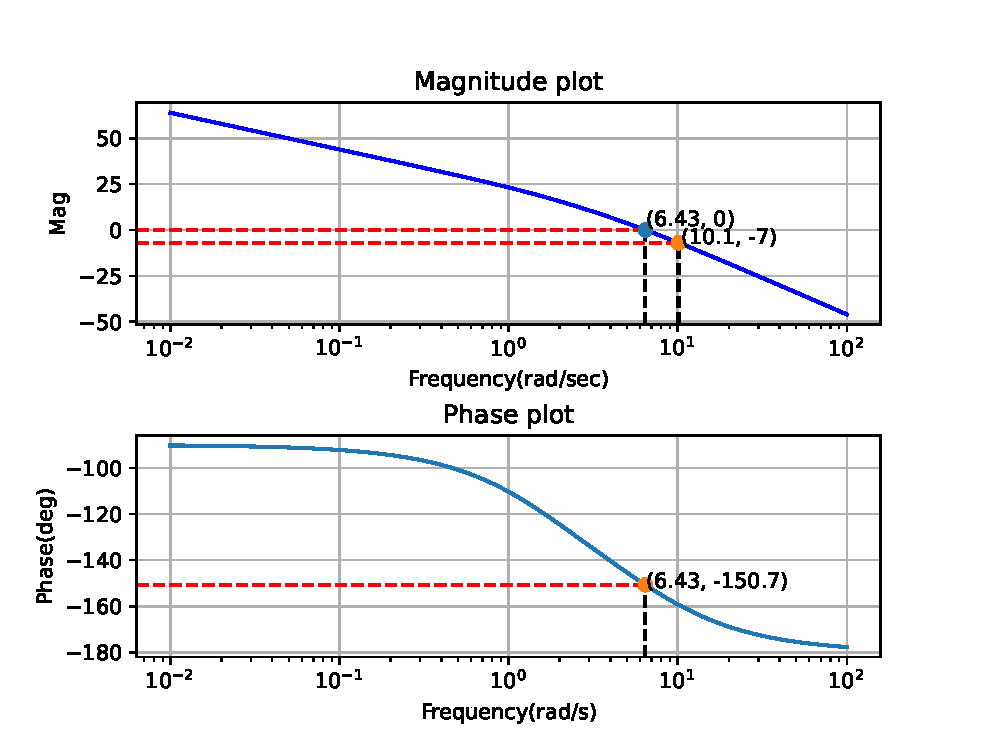
\includegraphics[width=\columnwidth]{./figs/ee18btech11047/ee18btech11047_2.eps}
\caption{1}
\label{fig:ee18btech11047_2}
\end{figure}
The phase margin is 
\begin{align}
\phi_{M} &= 180\degree-150.7\degree \implies \phi_{M} = 29.3\degree \label{eq:ee18btech11047_ph}
\end{align}
The closed-loop bandwith, $\omega_{BW}$(-3 dB frequency), equals the frequency at which the open-loop magnitude response is around -7 dB.
\begin{align}
\omega_{BW} = 10.1  rad/sec \label{eq:ee18btech11047_bw}
\end{align}
\textbf{Damping ratio:} \\
Substitute $\phi_{M}$ value from equation(\ref{eq:ee18btech11047_ph})
\begin{align}
\phi_{M} &= {tan}^{-1}\brak{\frac{2\zeta}{\sqrt{-2\zeta^{2}+\sqrt{1+4\zeta^{2}}}}}\\
\implies \zeta &= 0.34
\end{align}
\textbf{Settling time:} \\
Substitute $\omega_{BW}$ value from equation(\ref{eq:ee18btech11047_bw}) and $\zeta$
\begin{align}
T_{s}&= \frac{4}{\omega_{BW}\zeta}\sqrt{(1-2\zeta^2)+\sqrt{4\zeta^4-4\zeta^2+2}}\\
\implies T_{s} &= 1.65 sec   \\
\end{align}
\textbf{Peak time:}
\begin{align}
T_{p} &= \frac{\pi\zeta T_{s}}{4\sqrt{1-\zeta^2}}\\
\implies T_{p} &= 0.325 sec
\end{align}
\textbf{Percent overshoot:}
\begin{align}
\% OS&=100e^{-(\frac{\zeta\pi}{\sqrt{1-\zeta^2}})}\\
\implies \% OS &= 35.1 \%
\end{align}
Note that the answers will be approximate due to the dominant pole approximation.\\
The following code generates the step response of the system.
\begin{lstlisting}
codes/ee18btech11047/ee18btech11047_3.py
\end{lstlisting}
\begin{figure}[!ht]
\centering
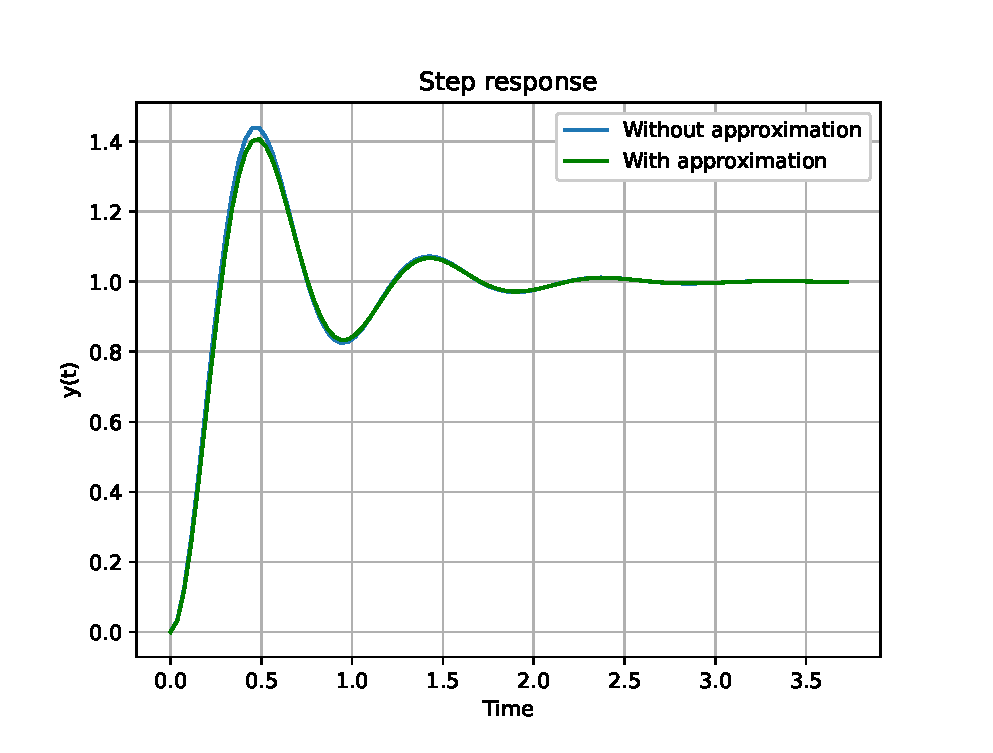
\includegraphics[width=\columnwidth]{./figs/ee18btech11047/ee18btech11047_3.eps}
\caption{2}
\label{fig:ee18btech11047_3}
\end{figure}
\item Find the approximate transfer function for the open loop transfer function
\begin{align}
G(s) &= \frac{75(1+0.2s)}{s(s^{2}+16s+100)}
\end{align}
\solution Using equation \eqref{eq:ee18btech11047_ctf}
\begin{align}
T(s) = \frac{75(1+0.2s)}{s^3 + 16s^2 + 115s +75} 
\end{align}
The following code gives the poles and zeros of the transfer function.
\begin{lstlisting}
codes/ee18btech11047/ee18btech11047_4.py
\end{lstlisting}
\begin{table}[!ht]
\centering
\input{./tables/ee18btech11047/ee18btech11047_2.tex}
\caption{}
\label{table:ee18btech11047_2}
\end{table}
The real part of the complex conjugate poles is comparable with the zero $z_{1}$ of the transfer function.So,they cancel out each other.
The approximated transfer function is of first order.
\begin{align}
T_{2}(s) &= \frac{K_{2}}{(s-p_{1})}\\
T(0) &= T_{2}(s)\\
\implies K_{2} &= p_{1} \\
T_{2}(s) &= \frac{0.72}{s+0.72}
\end{align}
\item Estimate the transient response of the obtained first order system.\\
\solution\\
\textbf{Time constant:}\\
The time constant is the time taken by the step response to rise to 63\% of it's final value.
\begin{align}
T &= \frac{1}{|pole|}\\
T &= \frac{1}{0.72} = 1.388 sec
\end{align}
\textbf{Rise time:}\\
Rise time is the time for the waveform to go from 0.1 to 0.9 of it's final value.
\begin{align}
T_{r} &= \frac{2.2}{|pole|}\\
T_{r} &= \frac{2.2}{0.72} = 3.05 sec
\end{align}
\textbf{Settling time:}\\
Settling time is defined as the time for the response to reach and stay within, 2\% of its final value.
\begin{align}
T_{s} &= \frac{4}{|pole|}\\
T_{s} &= \frac{4}{0.72}=5.55 sec
\end{align}
The following code plots the step response of the system.
\begin{lstlisting}
codes/ee18btech11047/ee18btech11047_5.py
\end{lstlisting}
\begin{figure}[!ht]
\centering
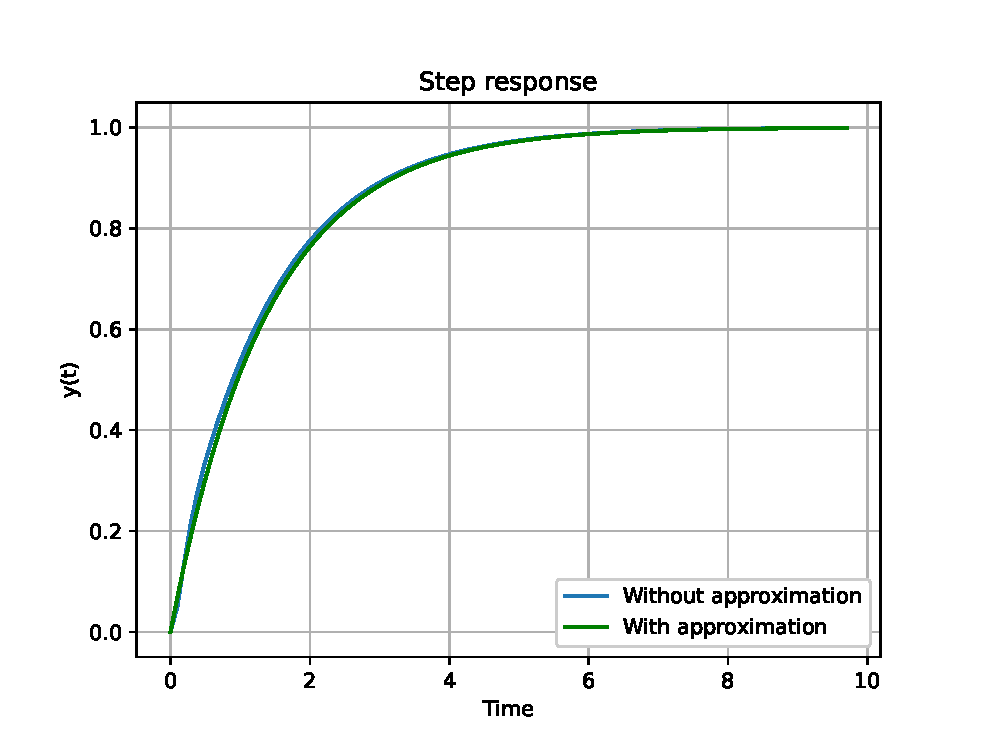
\includegraphics[width=\columnwidth]{./figs/ee18btech11047/ee18btech11047_4.eps}
\caption{}
\label{fig:ee18btech11047_4}
\end{figure}
\end{enumerate}

\caption{}
\label{table:ee18btech11047}
\end{table}
The real poles \brak{p_{1},p_{2}} and zeros \brak{z_{1},z_{2}} cancel out each other as mentioned above.So, we are left with the two conjugate poles.\\
The approximated transfer function is 
\begin{align}
T_{1}(s) &= \frac{K_{1}}{(s-p_{3})(s-p_{4})}\\ 
T(0) &= T_{1}(0)\\
\implies K_{1} &= p_{3}p_{4}\\
T_{1}(s) &= \frac{47.09}{s^{2}+3.74s+47.09}
\end{align}
\item Estimate the transient response of the obtained second order system using the respective bode plot.\\
\solution The following code generates the bode plot for open loop transfer function.
\begin{lstlisting}
codes/ee18btech11047/ee18btech11047_2.py
\end{lstlisting}
\begin{figure}[!ht]
\centering
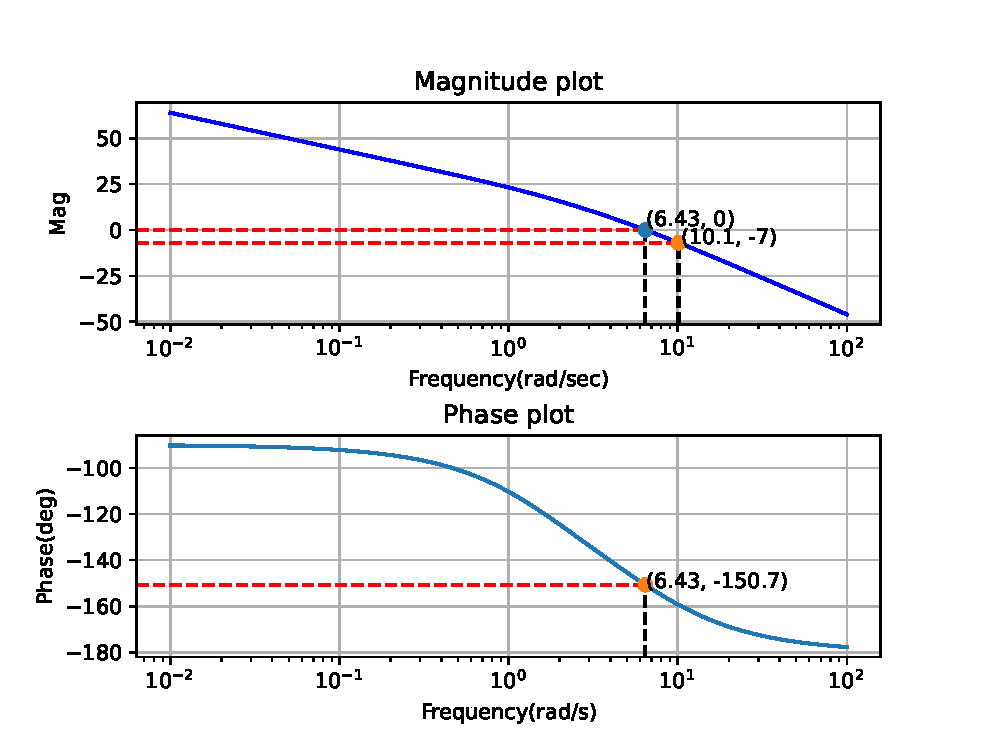
\includegraphics[width=\columnwidth]{./figs/ee18btech11047/ee18btech11047_2.eps}
\caption{1}
\label{fig:ee18btech11047_2}
\end{figure}
The phase margin is 
\begin{align}
\phi_{M} &= 180\degree-150.7\degree \implies \phi_{M} = 29.3\degree \label{eq:ee18btech11047_ph}
\end{align}
The closed-loop bandwith, $\omega_{BW}$(-3 dB frequency), equals the frequency at which the open-loop magnitude response is around -7 dB.
\begin{align}
\omega_{BW} = 10.1  rad/sec \label{eq:ee18btech11047_bw}
\end{align}
\textbf{Damping ratio:} \\
Substitute $\phi_{M}$ value from equation(\ref{eq:ee18btech11047_ph})
\begin{align}
\phi_{M} &= {tan}^{-1}\brak{\frac{2\zeta}{\sqrt{-2\zeta^{2}+\sqrt{1+4\zeta^{2}}}}}\\
\implies \zeta &= 0.34
\end{align}
\textbf{Settling time:} \\
Substitute $\omega_{BW}$ value from equation(\ref{eq:ee18btech11047_bw}) and $\zeta$
\begin{align}
T_{s}&= \frac{4}{\omega_{BW}\zeta}\sqrt{(1-2\zeta^2)+\sqrt{4\zeta^4-4\zeta^2+2}}\\
\implies T_{s} &= 1.65 sec   \\
\end{align}
\textbf{Peak time:}
\begin{align}
T_{p} &= \frac{\pi\zeta T_{s}}{4\sqrt{1-\zeta^2}}\\
\implies T_{p} &= 0.325 sec
\end{align}
\textbf{Percent overshoot:}
\begin{align}
\% OS&=100e^{-(\frac{\zeta\pi}{\sqrt{1-\zeta^2}})}\\
\implies \% OS &= 35.1 \%
\end{align}
Note that the answers will be approximate due to the dominant pole approximation.\\
The following code generates the step response of the system.
\begin{lstlisting}
codes/ee18btech11047/ee18btech11047_3.py
\end{lstlisting}
\begin{figure}[!ht]
\centering
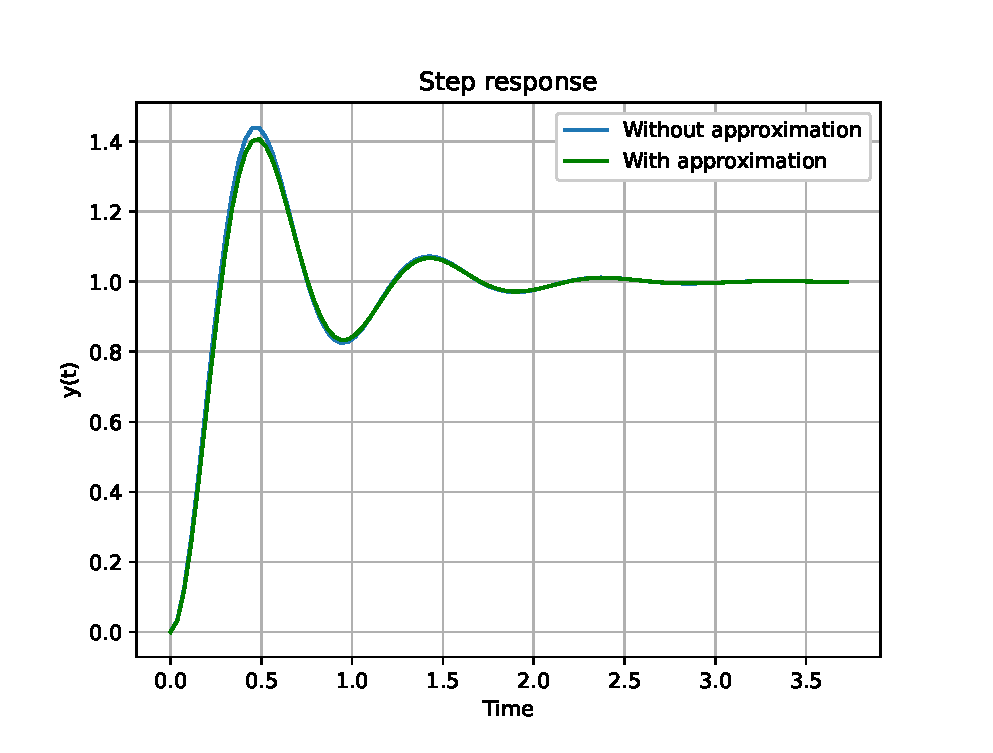
\includegraphics[width=\columnwidth]{./figs/ee18btech11047/ee18btech11047_3.eps}
\caption{2}
\label{fig:ee18btech11047_3}
\end{figure}
\item Find the approximate transfer function for the open loop transfer function
\begin{align}
G(s) &= \frac{75(1+0.2s)}{s(s^{2}+16s+100)}
\end{align}
\solution Using equation \eqref{eq:ee18btech11047_ctf}
\begin{align}
T(s) = \frac{75(1+0.2s)}{s^3 + 16s^2 + 115s +75} 
\end{align}
The following code gives the poles and zeros of the transfer function.
\begin{lstlisting}
codes/ee18btech11047/ee18btech11047_4.py
\end{lstlisting}
\begin{table}[!ht]
\centering
\tikzstyle{block} = [draw, fill=blue!20, rectangle, 
    minimum height=3em, minimum width=6em]
\tikzstyle{sum} = [draw, fill=blue!20, circle, node distance=1cm]
\tikzstyle{input} = [coordinate]
\tikzstyle{output} = [coordinate]
\tikzstyle{pinstyle} = [pin edge={to-,thin,black}]

\begin{tikzpicture}[auto, node distance=2cm,>=latex']
    \node [input, name=input] {};
    \node [sum, right of=input] (sum) {};
    \node [block, right of=sum] (controller) {$G$};
    \node [output, right of=controller] (output) {};
    \node [block, below of=controller] (feedback) {$H$};
    \draw [draw,->] (input) -- node {} (sum);
    \draw [->] (sum) -- node {$V_i$} (controller);
    \draw [->] (controller) -- node [name=y] {$V_o$}(output);
    \draw [->] (y) |- (feedback);
    \draw [->] (feedback) -| node[pos=0.99]{$+$}  node [near end] {$V_f$} (sum);
\end{tikzpicture}

\caption{}
\label{table:ee18btech11047_2}
\end{table}
The real part of the complex conjugate poles is comparable with the zero $z_{1}$ of the transfer function.So,they cancel out each other.
The approximated transfer function is of first order.
\begin{align}
T_{2}(s) &= \frac{K_{2}}{(s-p_{1})}\\
T(0) &= T_{2}(s)\\
\implies K_{2} &= p_{1} \\
T_{2}(s) &= \frac{0.72}{s+0.72}
\end{align}
\item Estimate the transient response of the obtained first order system.\\
\solution\\
\textbf{Time constant:}\\
The time constant is the time taken by the step response to rise to 63\% of it's final value.
\begin{align}
T &= \frac{1}{|pole|}\\
T &= \frac{1}{0.72} = 1.388 sec
\end{align}
\textbf{Rise time:}\\
Rise time is the time for the waveform to go from 0.1 to 0.9 of it's final value.
\begin{align}
T_{r} &= \frac{2.2}{|pole|}\\
T_{r} &= \frac{2.2}{0.72} = 3.05 sec
\end{align}
\textbf{Settling time:}\\
Settling time is defined as the time for the response to reach and stay within, 2\% of its final value.
\begin{align}
T_{s} &= \frac{4}{|pole|}\\
T_{s} &= \frac{4}{0.72}=5.55 sec
\end{align}
The following code plots the step response of the system.
\begin{lstlisting}
codes/ee18btech11047/ee18btech11047_5.py
\end{lstlisting}
\begin{figure}[!ht]
\centering
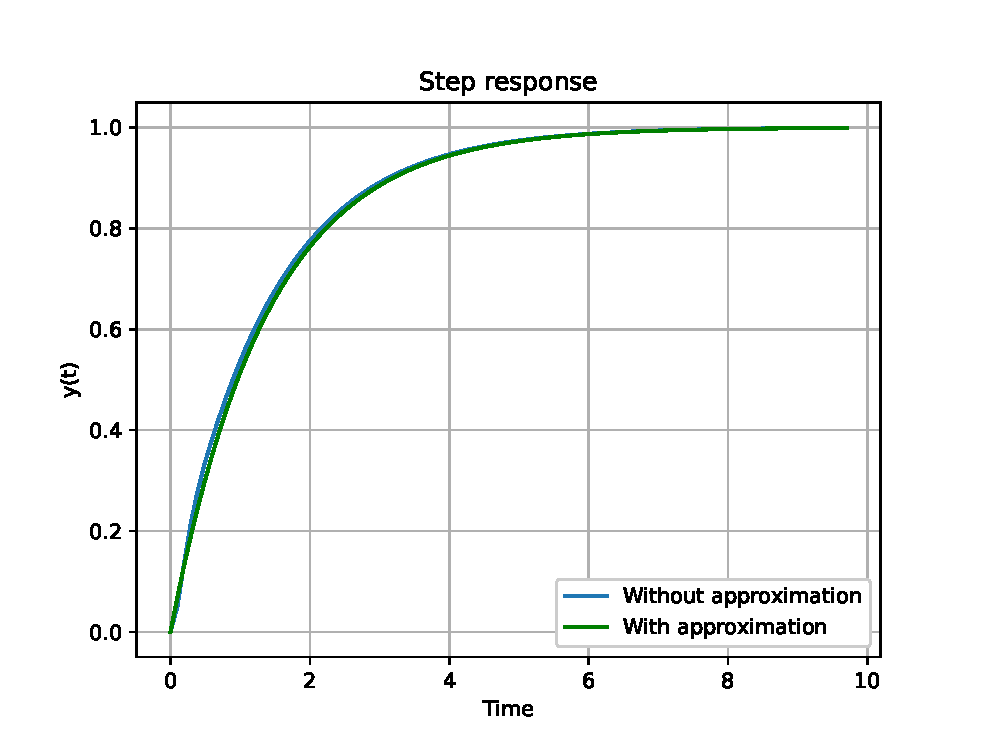
\includegraphics[width=\columnwidth]{./figs/ee18btech11047/ee18btech11047_4.eps}
\caption{}
\label{fig:ee18btech11047_4}
\end{figure}
\end{enumerate}

\caption{}
\label{table:ee18btech11047}
\end{table}
The real poles \brak{p_{1},p_{2}} and zeros \brak{z_{1},z_{2}} cancel out each other as mentioned above.So, we are left with the two conjugate poles.\\
The approximated transfer function is 
\begin{align}
T_{1}(s) &= \frac{K_{1}}{(s-p_{3})(s-p_{4})}\\ 
T(0) &= T_{1}(0)\\
\implies K_{1} &= p_{3}p_{4}\\
T_{1}(s) &= \frac{47.09}{s^{2}+3.74s+47.09}
\end{align}
\item Estimate the transient response of the obtained second order system using the respective bode plot.\\
\solution The following code generates the bode plot for open loop transfer function.
\begin{lstlisting}
codes/ee18btech11047/ee18btech11047_2.py
\end{lstlisting}
\begin{figure}[!ht]
\centering
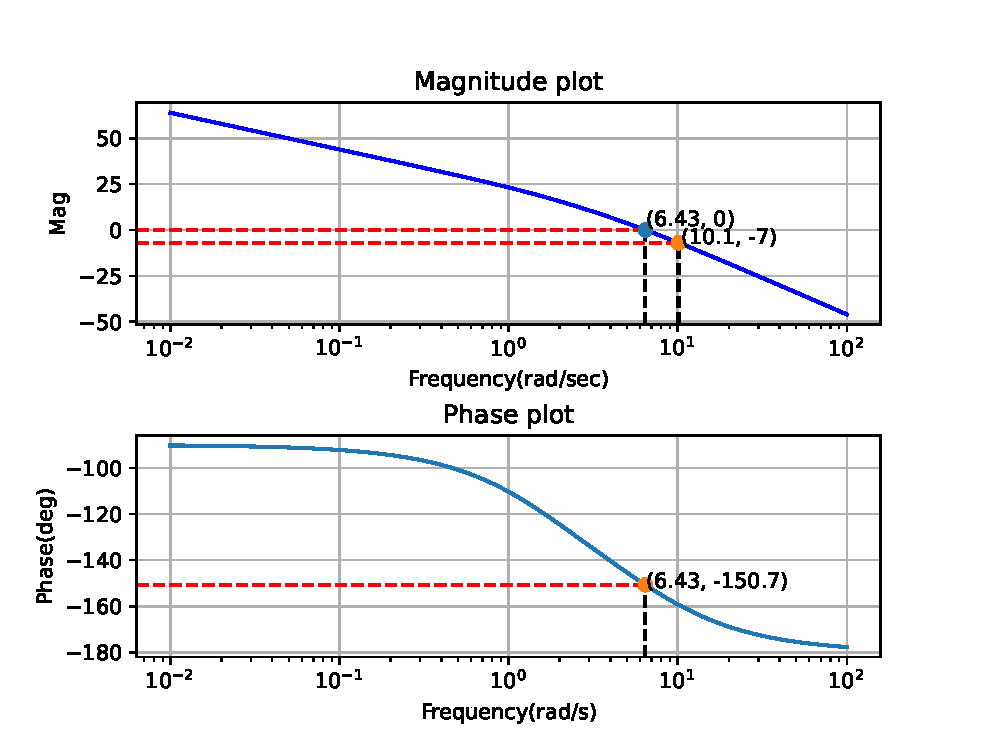
\includegraphics[width=\columnwidth]{./figs/ee18btech11047/ee18btech11047_2.eps}
\caption{1}
\label{fig:ee18btech11047_2}
\end{figure}
The phase margin is 
\begin{align}
\phi_{M} &= 180\degree-150.7\degree \implies \phi_{M} = 29.3\degree \label{eq:ee18btech11047_ph}
\end{align}
The closed-loop bandwith, $\omega_{BW}$(-3 dB frequency), equals the frequency at which the open-loop magnitude response is around -7 dB.
\begin{align}
\omega_{BW} = 10.1  rad/sec \label{eq:ee18btech11047_bw}
\end{align}
\textbf{Damping ratio:} \\
Substitute $\phi_{M}$ value from equation(\ref{eq:ee18btech11047_ph})
\begin{align}
\phi_{M} &= {tan}^{-1}\brak{\frac{2\zeta}{\sqrt{-2\zeta^{2}+\sqrt{1+4\zeta^{2}}}}}\\
\implies \zeta &= 0.34
\end{align}
\textbf{Settling time:} \\
Substitute $\omega_{BW}$ value from equation(\ref{eq:ee18btech11047_bw}) and $\zeta$
\begin{align}
T_{s}&= \frac{4}{\omega_{BW}\zeta}\sqrt{(1-2\zeta^2)+\sqrt{4\zeta^4-4\zeta^2+2}}\\
\implies T_{s} &= 1.65 sec   \\
\end{align}
\textbf{Peak time:}
\begin{align}
T_{p} &= \frac{\pi\zeta T_{s}}{4\sqrt{1-\zeta^2}}\\
\implies T_{p} &= 0.325 sec
\end{align}
\textbf{Percent overshoot:}
\begin{align}
\% OS&=100e^{-(\frac{\zeta\pi}{\sqrt{1-\zeta^2}})}\\
\implies \% OS &= 35.1 \%
\end{align}
Note that the answers will be approximate due to the dominant pole approximation.\\
The following code generates the step response of the system.
\begin{lstlisting}
codes/ee18btech11047/ee18btech11047_3.py
\end{lstlisting}
\begin{figure}[!ht]
\centering
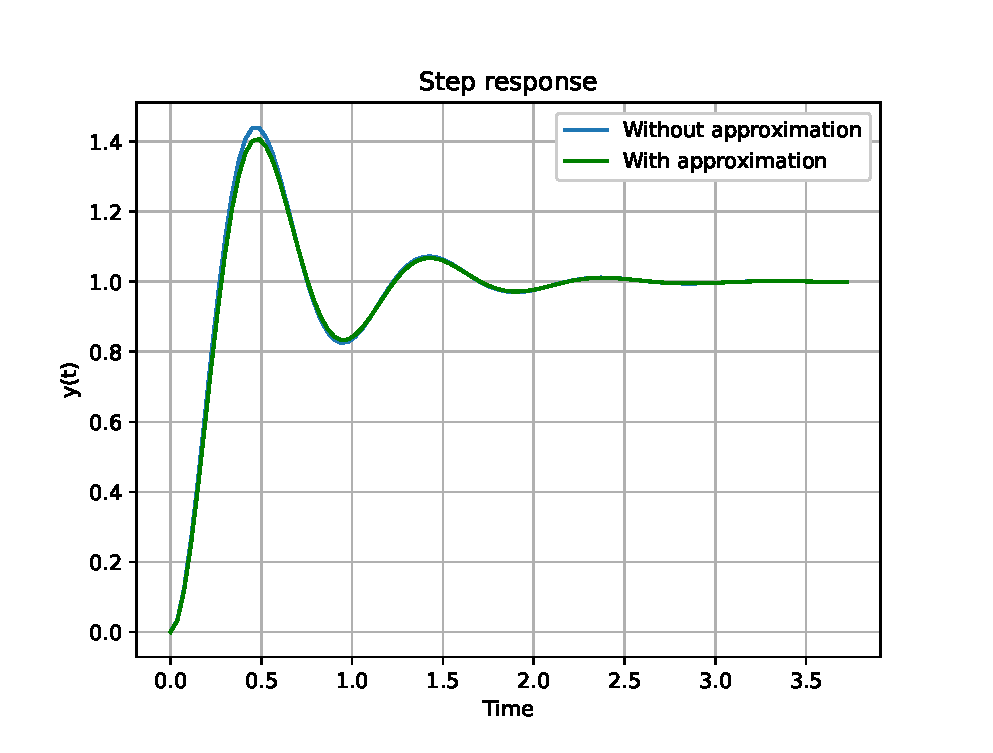
\includegraphics[width=\columnwidth]{./figs/ee18btech11047/ee18btech11047_3.eps}
\caption{2}
\label{fig:ee18btech11047_3}
\end{figure}
\item Find the approximate transfer function for the open loop transfer function
\begin{align}
G(s) &= \frac{75(1+0.2s)}{s(s^{2}+16s+100)}
\end{align}
\solution Using equation \eqref{eq:ee18btech11047_ctf}
\begin{align}
T(s) = \frac{75(1+0.2s)}{s^3 + 16s^2 + 115s +75} 
\end{align}
The following code gives the poles and zeros of the transfer function.
\begin{lstlisting}
codes/ee18btech11047/ee18btech11047_4.py
\end{lstlisting}
\begin{table}[!ht]
\centering
\tikzstyle{block} = [draw, fill=blue!20, rectangle, 
    minimum height=3em, minimum width=6em]
\tikzstyle{sum} = [draw, fill=blue!20, circle, node distance=1cm]
\tikzstyle{input} = [coordinate]
\tikzstyle{output} = [coordinate]
\tikzstyle{pinstyle} = [pin edge={to-,thin,black}]

\begin{tikzpicture}[auto, node distance=2cm,>=latex']
    \node [input, name=input] {};
    \node [sum, right of=input] (sum) {};
    \node [block, right of=sum] (controller) {$G$};
    \node [output, right of=controller] (output) {};
    \node [block, below of=controller] (feedback) {$H$};
    \draw [draw,->] (input) -- node {} (sum);
    \draw [->] (sum) -- node {$V_i$} (controller);
    \draw [->] (controller) -- node [name=y] {$V_o$}(output);
    \draw [->] (y) |- (feedback);
    \draw [->] (feedback) -| node[pos=0.99]{$+$}  node [near end] {$V_f$} (sum);
\end{tikzpicture}

\caption{}
\label{table:ee18btech11047_2}
\end{table}
The real part of the complex conjugate poles is comparable with the zero $z_{1}$ of the transfer function.So,they cancel out each other.
The approximated transfer function is of first order.
\begin{align}
T_{2}(s) &= \frac{K_{2}}{(s-p_{1})}\\
T(0) &= T_{2}(s)\\
\implies K_{2} &= p_{1} \\
T_{2}(s) &= \frac{0.72}{s+0.72}
\end{align}
\item Estimate the transient response of the obtained first order system.\\
\solution\\
\textbf{Time constant:}\\
The time constant is the time taken by the step response to rise to 63\% of it's final value.
\begin{align}
T &= \frac{1}{|pole|}\\
T &= \frac{1}{0.72} = 1.388 sec
\end{align}
\textbf{Rise time:}\\
Rise time is the time for the waveform to go from 0.1 to 0.9 of it's final value.
\begin{align}
T_{r} &= \frac{2.2}{|pole|}\\
T_{r} &= \frac{2.2}{0.72} = 3.05 sec
\end{align}
\textbf{Settling time:}\\
Settling time is defined as the time for the response to reach and stay within, 2\% of its final value.
\begin{align}
T_{s} &= \frac{4}{|pole|}\\
T_{s} &= \frac{4}{0.72}=5.55 sec
\end{align}
The following code plots the step response of the system.
\begin{lstlisting}
codes/ee18btech11047/ee18btech11047_5.py
\end{lstlisting}
\begin{figure}[!ht]
\centering
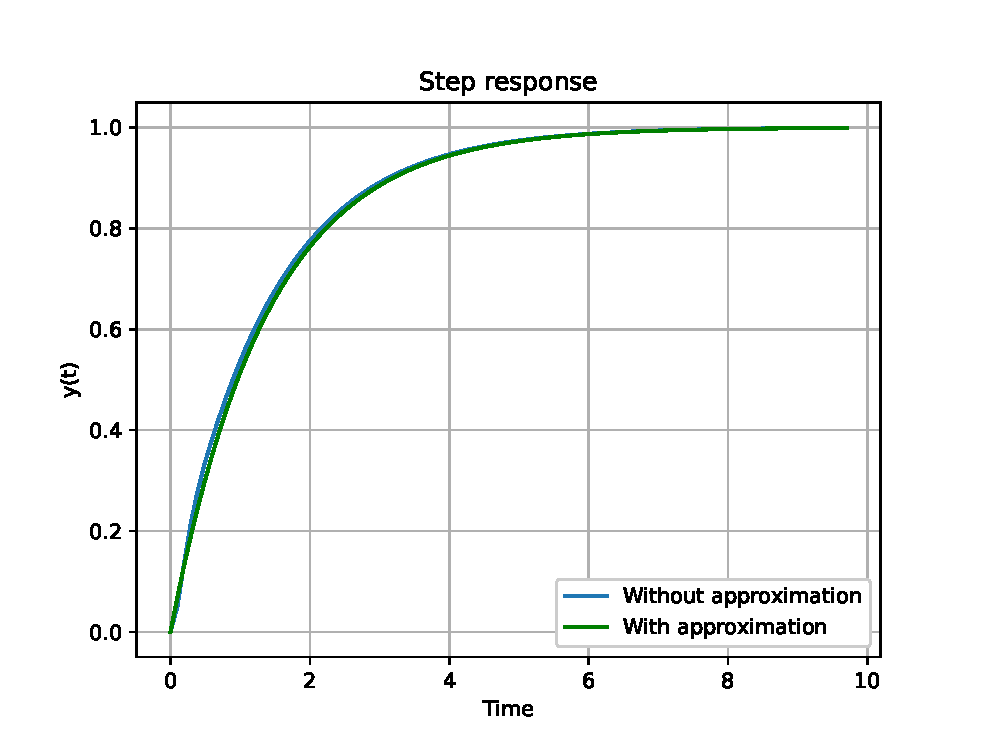
\includegraphics[width=\columnwidth]{./figs/ee18btech11047/ee18btech11047_4.eps}
\caption{}
\label{fig:ee18btech11047_4}
\end{figure}
\end{enumerate}
}
	\end{center}
\caption{}
\label{fig:ee18btech11047}
\end{figure}
Given open loop transfer function.The closed loop transfer function for a negative unity feedback system is
\begin{align}
T(s) &= \frac{G(s)}{1+G(s)} \label{eq:ee18btech11047_tf}
\end{align}
\item Find the approximate transfer function for the open loop transfer function
\begin{align}
G(s) &= \frac{50(s+3)(s+5)}{s(s+2)(s+4)(s+6)} \label{eq:ee18btech11047_1}
\end{align}
\solution Using equation(\ref{eq:ee18btech11047_tf})
\begin{align}
T(s) &= \frac{50(s^{2}+8s+15)}{s^4+12s^3+94s^2+448s+750} \label{eq:ee18btech11047_tf1}
\end{align}
The following code gives the poles and zeros of the transfer function.
\begin{lstlisting}
codes/ee18btech11047/ee18btech11047_1.py
\end{lstlisting}
\begin{table}[!ht]
\centering
\begin{enumerate}[label=\thesubsection.\arabic*.,ref=\thesubsection.\theenumi]
\numberwithin{equation}{enumi}

\item Consider the following transfer functions as open-loop transfer functions in two different unity feedback(negative) systems.
\begin{align}
G(s) &= \frac{50(s+3)(s+5)}{s(s+2)(s+4)(s+6)} 
\\
G(s) &= \frac{75(1+0.2s)}{s(s^{2}+16s+100)} 
\end{align}
Estimate transient response of these systems from their respective bode plots.
\\
\solution 
\begin{enumerate}
\item  The dominant pole approximation is used to characterize higher order systems because it is difficult to characterize and analyse systems with order greater than 3.
\item Consider a transfer function.
\begin{align}
H(s) = K\frac{\alpha\beta}{(s+\alpha)(s+\beta)}
\end{align}
It has two poles $-\alpha$ and $-\beta $. If the magnitude of $\beta$ is very large compared to $\alpha$ (typically if $\frac{|\beta|}{|\alpha|}$ $>$ 5  ) we can approximate for the transfer function assuming $s$ is sufficiently small compared to $\beta$ as follows.
\begin{align}
H(s) = K_{2}\brak{\frac{1}{s+\alpha}}
\end{align}
Note that the value of $H(0)$ should be unchanged for the exact and approximate transfer functions.This is necessary to ensure that the final value of the step response is unchanged.
\begin{align}
\lim_{t\to\infty} y(t) &= \lim_{s\to 0} sY(s) \\
\lim_{t\to\infty} y(t) &= \lim_{s\to 0} sU(s)H(s) = H(0)
\end{align}
In order to acheive this we adjust the gain value of the approximated transfer function by equating $H(0)$ values.
\begin{align}
\implies H(s) = K\frac{\alpha}{(s+\alpha)}
\end{align}
\item In terms of poles, the pole closer to the origin is considered as the dominating pole.As considered above,the magnitude of $\alpha$ is small therefore the time constant $\frac{1}{\alpha}$ will be high and reaches equilibrium slowly and vice versa in case of  $\beta$.Therefore,this approximation assumes that the slowest part of the system dominates the response.The faster parts of the system are ignored.
\item Complex poles along with real poles : In this case the dominant pole(s) can be determined by comparing only the real parts.If the real part of the complex conjugate poles is greater in magnitude than the real pole, the two complex conjugate poles the dominant poles.
\item If the transfer function has zeros along with poles,we have to consider the fact that pole and zero cancel out each other if their respective magnitudes are comparable.
\end{enumerate}
\item Find the closed loop transfer function of a negative unity feedback system given open loop transfer function $G(s)$ .\\
\solution 
\begin{align}
\label{eq:ee18btech11047_ctf}
T(s) &= \frac{G(s)}{1+G(s)}
\end{align}
\begin{figure}[!ht]
	\begin{center}
		\resizebox{\columnwidth}{!}{\begin{enumerate}[label=\thesubsection.\arabic*.,ref=\thesubsection.\theenumi]
\numberwithin{equation}{enumi}

\item Consider the following transfer functions as open-loop transfer functions in two different unity feedback(negative) systems.
\begin{align}
G(s) &= \frac{50(s+3)(s+5)}{s(s+2)(s+4)(s+6)} 
\\
G(s) &= \frac{75(1+0.2s)}{s(s^{2}+16s+100)} 
\end{align}
Estimate transient response of these systems from their respective bode plots.
\\
\solution 
\begin{enumerate}
\item  The dominant pole approximation is used to characterize higher order systems because it is difficult to characterize and analyse systems with order greater than 3.
\item Consider a transfer function.
\begin{align}
H(s) = K\frac{\alpha\beta}{(s+\alpha)(s+\beta)}
\end{align}
It has two poles $-\alpha$ and $-\beta $. If the magnitude of $\beta$ is very large compared to $\alpha$ (typically if $\frac{|\beta|}{|\alpha|}$ $>$ 5  ) we can approximate for the transfer function assuming $s$ is sufficiently small compared to $\beta$ as follows.
\begin{align}
H(s) = K_{2}\brak{\frac{1}{s+\alpha}}
\end{align}
Note that the value of $H(0)$ should be unchanged for the exact and approximate transfer functions.This is necessary to ensure that the final value of the step response is unchanged.
\begin{align}
\lim_{t\to\infty} y(t) &= \lim_{s\to 0} sY(s) \\
\lim_{t\to\infty} y(t) &= \lim_{s\to 0} sU(s)H(s) = H(0)
\end{align}
In order to acheive this we adjust the gain value of the approximated transfer function by equating $H(0)$ values.
\begin{align}
\implies H(s) = K\frac{\alpha}{(s+\alpha)}
\end{align}
\item In terms of poles, the pole closer to the origin is considered as the dominating pole.As considered above,the magnitude of $\alpha$ is small therefore the time constant $\frac{1}{\alpha}$ will be high and reaches equilibrium slowly and vice versa in case of  $\beta$.Therefore,this approximation assumes that the slowest part of the system dominates the response.The faster parts of the system are ignored.
\item Complex poles along with real poles : In this case the dominant pole(s) can be determined by comparing only the real parts.If the real part of the complex conjugate poles is greater in magnitude than the real pole, the two complex conjugate poles the dominant poles.
\item If the transfer function has zeros along with poles,we have to consider the fact that pole and zero cancel out each other if their respective magnitudes are comparable.
\end{enumerate}
\item Find the closed loop transfer function of a negative unity feedback system given open loop transfer function $G(s)$ .\\
\solution 
\begin{align}
\label{eq:ee18btech11047_ctf}
T(s) &= \frac{G(s)}{1+G(s)}
\end{align}
\begin{figure}[!ht]
	\begin{center}
		\resizebox{\columnwidth}{!}{\begin{enumerate}[label=\thesubsection.\arabic*.,ref=\thesubsection.\theenumi]
\numberwithin{equation}{enumi}

\item Consider the following transfer functions as open-loop transfer functions in two different unity feedback(negative) systems.
\begin{align}
G(s) &= \frac{50(s+3)(s+5)}{s(s+2)(s+4)(s+6)} 
\\
G(s) &= \frac{75(1+0.2s)}{s(s^{2}+16s+100)} 
\end{align}
Estimate transient response of these systems from their respective bode plots.
\\
\solution 
\begin{enumerate}
\item  The dominant pole approximation is used to characterize higher order systems because it is difficult to characterize and analyse systems with order greater than 3.
\item Consider a transfer function.
\begin{align}
H(s) = K\frac{\alpha\beta}{(s+\alpha)(s+\beta)}
\end{align}
It has two poles $-\alpha$ and $-\beta $. If the magnitude of $\beta$ is very large compared to $\alpha$ (typically if $\frac{|\beta|}{|\alpha|}$ $>$ 5  ) we can approximate for the transfer function assuming $s$ is sufficiently small compared to $\beta$ as follows.
\begin{align}
H(s) = K_{2}\brak{\frac{1}{s+\alpha}}
\end{align}
Note that the value of $H(0)$ should be unchanged for the exact and approximate transfer functions.This is necessary to ensure that the final value of the step response is unchanged.
\begin{align}
\lim_{t\to\infty} y(t) &= \lim_{s\to 0} sY(s) \\
\lim_{t\to\infty} y(t) &= \lim_{s\to 0} sU(s)H(s) = H(0)
\end{align}
In order to acheive this we adjust the gain value of the approximated transfer function by equating $H(0)$ values.
\begin{align}
\implies H(s) = K\frac{\alpha}{(s+\alpha)}
\end{align}
\item In terms of poles, the pole closer to the origin is considered as the dominating pole.As considered above,the magnitude of $\alpha$ is small therefore the time constant $\frac{1}{\alpha}$ will be high and reaches equilibrium slowly and vice versa in case of  $\beta$.Therefore,this approximation assumes that the slowest part of the system dominates the response.The faster parts of the system are ignored.
\item Complex poles along with real poles : In this case the dominant pole(s) can be determined by comparing only the real parts.If the real part of the complex conjugate poles is greater in magnitude than the real pole, the two complex conjugate poles the dominant poles.
\item If the transfer function has zeros along with poles,we have to consider the fact that pole and zero cancel out each other if their respective magnitudes are comparable.
\end{enumerate}
\item Find the closed loop transfer function of a negative unity feedback system given open loop transfer function $G(s)$ .\\
\solution 
\begin{align}
\label{eq:ee18btech11047_ctf}
T(s) &= \frac{G(s)}{1+G(s)}
\end{align}
\begin{figure}[!ht]
	\begin{center}
		\resizebox{\columnwidth}{!}{\input{./figs/ee18btech11047/ee18btech11047.tex}}
	\end{center}
\caption{}
\label{fig:ee18btech11047}
\end{figure}

\item Find the approximate transfer function for the open loop transfer function.
\begin{align}
G(s) &= \frac{50(s+3)(s+5)}{s(s+2)(s+4)(s+6)}
\end{align}
\solution Using equation\eqref{eq:ee18btech11047_ctf}
\begin{align}
T(s) &= \frac{50(s^{2}+8s+15)}{s^4+12s^3+94s^2+448s+750}
\end{align}
The following code gives the poles and zeros of the transfer function.
\begin{lstlisting}
codes/ee18btech11047/ee18btech11047_1.py
\end{lstlisting}
\begin{table}[!ht]
\centering
\input{./tables/ee18btech11047/ee18btech11047.tex}
\caption{}
\label{table:ee18btech11047}
\end{table}
The real poles \brak{p_{1},p_{2}} and zeros \brak{z_{1},z_{2}} cancel out each other as mentioned above.So, we are left with the two conjugate poles.\\
The approximated transfer function is 
\begin{align}
T_{1}(s) &= \frac{K_{1}}{(s-p_{3})(s-p_{4})}\\ 
T(0) &= T_{1}(0)\\
\implies K_{1} &= p_{3}p_{4}\\
T_{1}(s) &= \frac{47.09}{s^{2}+3.74s+47.09}
\end{align}
\item Estimate the transient response of the obtained second order system using the respective bode plot.\\
\solution The following code generates the bode plot for open loop transfer function.
\begin{lstlisting}
codes/ee18btech11047/ee18btech11047_2.py
\end{lstlisting}
\begin{figure}[!ht]
\centering
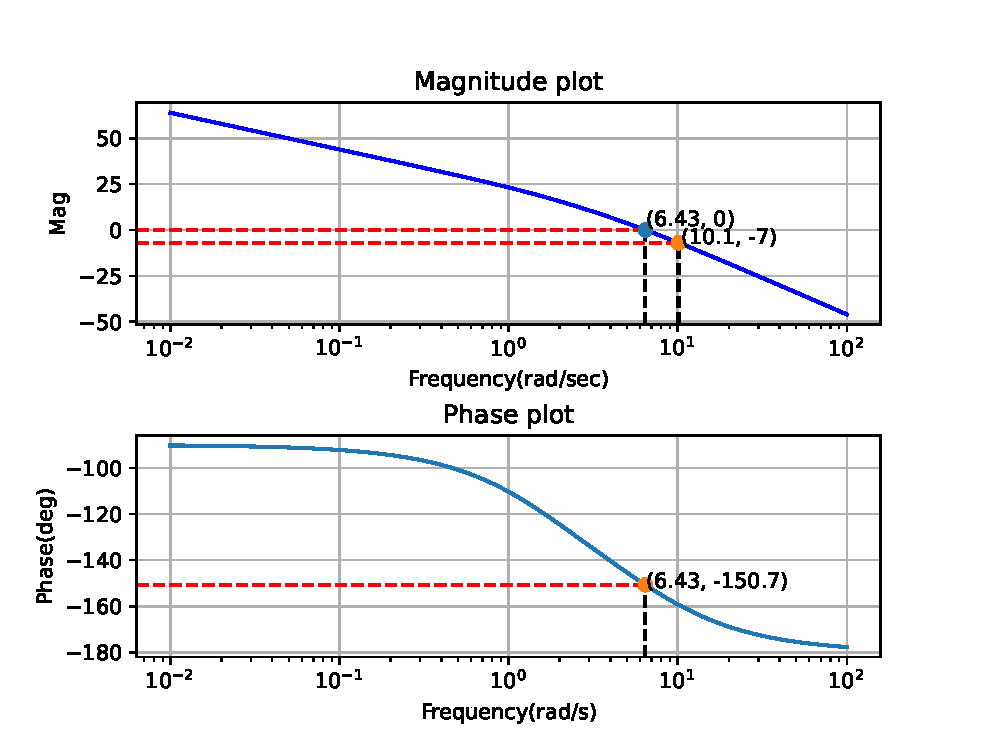
\includegraphics[width=\columnwidth]{./figs/ee18btech11047/ee18btech11047_2.eps}
\caption{1}
\label{fig:ee18btech11047_2}
\end{figure}
The phase margin is 
\begin{align}
\phi_{M} &= 180\degree-150.7\degree \implies \phi_{M} = 29.3\degree \label{eq:ee18btech11047_ph}
\end{align}
The closed-loop bandwith, $\omega_{BW}$(-3 dB frequency), equals the frequency at which the open-loop magnitude response is around -7 dB.
\begin{align}
\omega_{BW} = 10.1  rad/sec \label{eq:ee18btech11047_bw}
\end{align}
\textbf{Damping ratio:} \\
Substitute $\phi_{M}$ value from equation(\ref{eq:ee18btech11047_ph})
\begin{align}
\phi_{M} &= {tan}^{-1}\brak{\frac{2\zeta}{\sqrt{-2\zeta^{2}+\sqrt{1+4\zeta^{2}}}}}\\
\implies \zeta &= 0.34
\end{align}
\textbf{Settling time:} \\
Substitute $\omega_{BW}$ value from equation(\ref{eq:ee18btech11047_bw}) and $\zeta$
\begin{align}
T_{s}&= \frac{4}{\omega_{BW}\zeta}\sqrt{(1-2\zeta^2)+\sqrt{4\zeta^4-4\zeta^2+2}}\\
\implies T_{s} &= 1.65 sec   \\
\end{align}
\textbf{Peak time:}
\begin{align}
T_{p} &= \frac{\pi\zeta T_{s}}{4\sqrt{1-\zeta^2}}\\
\implies T_{p} &= 0.325 sec
\end{align}
\textbf{Percent overshoot:}
\begin{align}
\% OS&=100e^{-(\frac{\zeta\pi}{\sqrt{1-\zeta^2}})}\\
\implies \% OS &= 35.1 \%
\end{align}
Note that the answers will be approximate due to the dominant pole approximation.\\
The following code generates the step response of the system.
\begin{lstlisting}
codes/ee18btech11047/ee18btech11047_3.py
\end{lstlisting}
\begin{figure}[!ht]
\centering
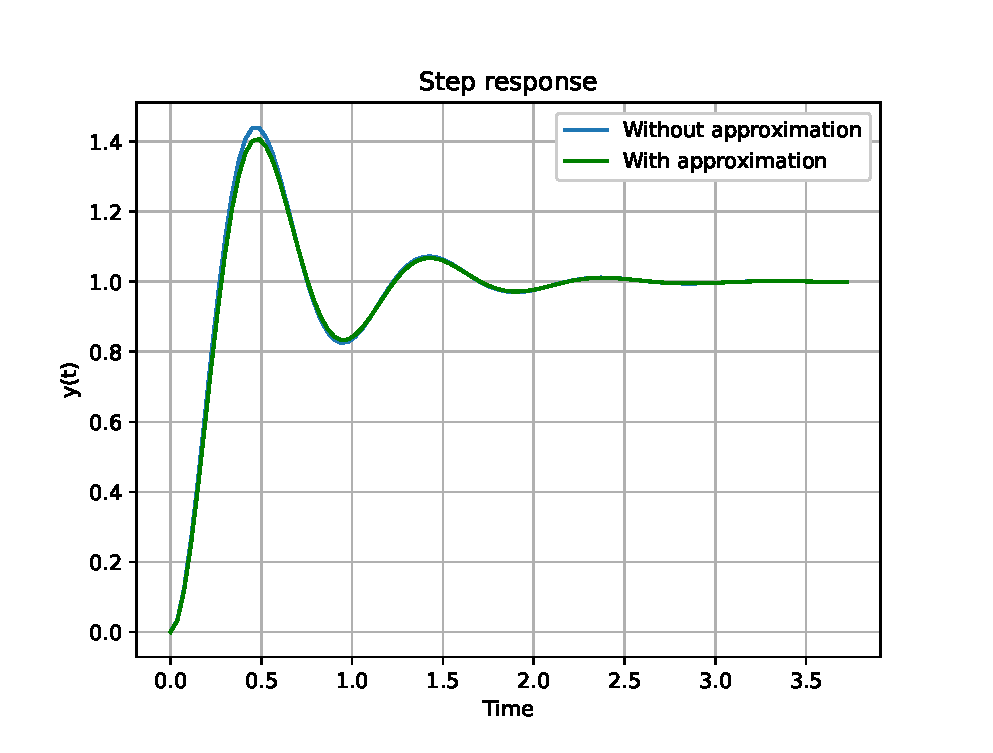
\includegraphics[width=\columnwidth]{./figs/ee18btech11047/ee18btech11047_3.eps}
\caption{2}
\label{fig:ee18btech11047_3}
\end{figure}
\item Find the approximate transfer function for the open loop transfer function
\begin{align}
G(s) &= \frac{75(1+0.2s)}{s(s^{2}+16s+100)}
\end{align}
\solution Using equation \eqref{eq:ee18btech11047_ctf}
\begin{align}
T(s) = \frac{75(1+0.2s)}{s^3 + 16s^2 + 115s +75} 
\end{align}
The following code gives the poles and zeros of the transfer function.
\begin{lstlisting}
codes/ee18btech11047/ee18btech11047_4.py
\end{lstlisting}
\begin{table}[!ht]
\centering
\input{./tables/ee18btech11047/ee18btech11047_2.tex}
\caption{}
\label{table:ee18btech11047_2}
\end{table}
The real part of the complex conjugate poles is comparable with the zero $z_{1}$ of the transfer function.So,they cancel out each other.
The approximated transfer function is of first order.
\begin{align}
T_{2}(s) &= \frac{K_{2}}{(s-p_{1})}\\
T(0) &= T_{2}(s)\\
\implies K_{2} &= p_{1} \\
T_{2}(s) &= \frac{0.72}{s+0.72}
\end{align}
\item Estimate the transient response of the obtained first order system.\\
\solution\\
\textbf{Time constant:}\\
The time constant is the time taken by the step response to rise to 63\% of it's final value.
\begin{align}
T &= \frac{1}{|pole|}\\
T &= \frac{1}{0.72} = 1.388 sec
\end{align}
\textbf{Rise time:}\\
Rise time is the time for the waveform to go from 0.1 to 0.9 of it's final value.
\begin{align}
T_{r} &= \frac{2.2}{|pole|}\\
T_{r} &= \frac{2.2}{0.72} = 3.05 sec
\end{align}
\textbf{Settling time:}\\
Settling time is defined as the time for the response to reach and stay within, 2\% of its final value.
\begin{align}
T_{s} &= \frac{4}{|pole|}\\
T_{s} &= \frac{4}{0.72}=5.55 sec
\end{align}
The following code plots the step response of the system.
\begin{lstlisting}
codes/ee18btech11047/ee18btech11047_5.py
\end{lstlisting}
\begin{figure}[!ht]
\centering
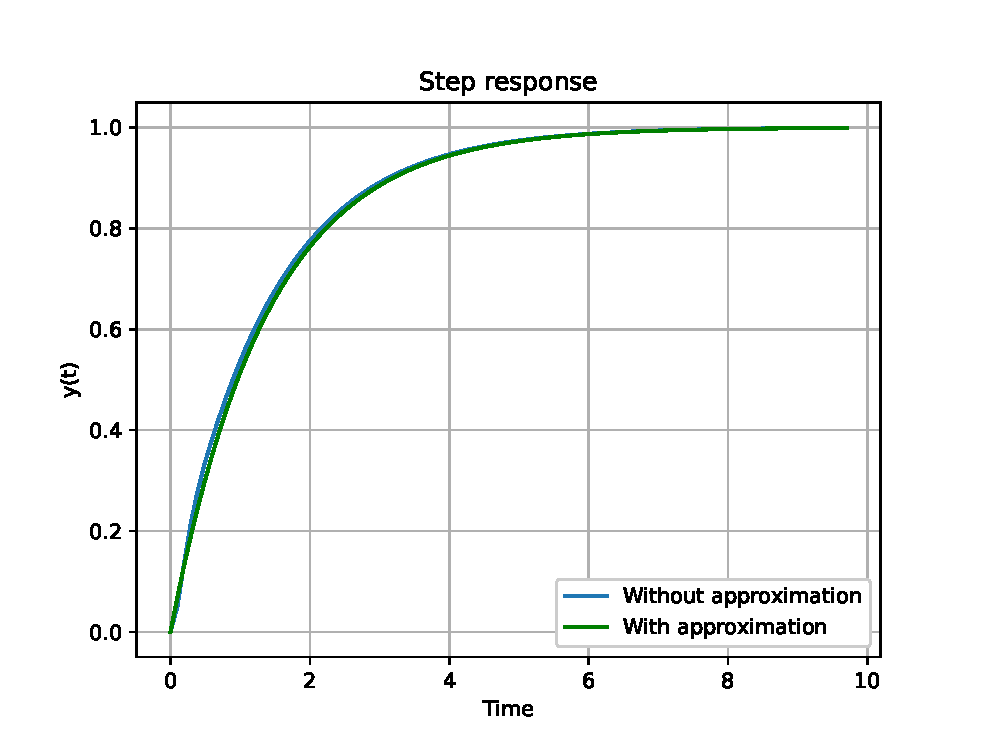
\includegraphics[width=\columnwidth]{./figs/ee18btech11047/ee18btech11047_4.eps}
\caption{}
\label{fig:ee18btech11047_4}
\end{figure}
\end{enumerate}
}
	\end{center}
\caption{}
\label{fig:ee18btech11047}
\end{figure}

\item Find the approximate transfer function for the open loop transfer function.
\begin{align}
G(s) &= \frac{50(s+3)(s+5)}{s(s+2)(s+4)(s+6)}
\end{align}
\solution Using equation\eqref{eq:ee18btech11047_ctf}
\begin{align}
T(s) &= \frac{50(s^{2}+8s+15)}{s^4+12s^3+94s^2+448s+750}
\end{align}
The following code gives the poles and zeros of the transfer function.
\begin{lstlisting}
codes/ee18btech11047/ee18btech11047_1.py
\end{lstlisting}
\begin{table}[!ht]
\centering
\begin{enumerate}[label=\thesubsection.\arabic*.,ref=\thesubsection.\theenumi]
\numberwithin{equation}{enumi}

\item Consider the following transfer functions as open-loop transfer functions in two different unity feedback(negative) systems.
\begin{align}
G(s) &= \frac{50(s+3)(s+5)}{s(s+2)(s+4)(s+6)} 
\\
G(s) &= \frac{75(1+0.2s)}{s(s^{2}+16s+100)} 
\end{align}
Estimate transient response of these systems from their respective bode plots.
\\
\solution 
\begin{enumerate}
\item  The dominant pole approximation is used to characterize higher order systems because it is difficult to characterize and analyse systems with order greater than 3.
\item Consider a transfer function.
\begin{align}
H(s) = K\frac{\alpha\beta}{(s+\alpha)(s+\beta)}
\end{align}
It has two poles $-\alpha$ and $-\beta $. If the magnitude of $\beta$ is very large compared to $\alpha$ (typically if $\frac{|\beta|}{|\alpha|}$ $>$ 5  ) we can approximate for the transfer function assuming $s$ is sufficiently small compared to $\beta$ as follows.
\begin{align}
H(s) = K_{2}\brak{\frac{1}{s+\alpha}}
\end{align}
Note that the value of $H(0)$ should be unchanged for the exact and approximate transfer functions.This is necessary to ensure that the final value of the step response is unchanged.
\begin{align}
\lim_{t\to\infty} y(t) &= \lim_{s\to 0} sY(s) \\
\lim_{t\to\infty} y(t) &= \lim_{s\to 0} sU(s)H(s) = H(0)
\end{align}
In order to acheive this we adjust the gain value of the approximated transfer function by equating $H(0)$ values.
\begin{align}
\implies H(s) = K\frac{\alpha}{(s+\alpha)}
\end{align}
\item In terms of poles, the pole closer to the origin is considered as the dominating pole.As considered above,the magnitude of $\alpha$ is small therefore the time constant $\frac{1}{\alpha}$ will be high and reaches equilibrium slowly and vice versa in case of  $\beta$.Therefore,this approximation assumes that the slowest part of the system dominates the response.The faster parts of the system are ignored.
\item Complex poles along with real poles : In this case the dominant pole(s) can be determined by comparing only the real parts.If the real part of the complex conjugate poles is greater in magnitude than the real pole, the two complex conjugate poles the dominant poles.
\item If the transfer function has zeros along with poles,we have to consider the fact that pole and zero cancel out each other if their respective magnitudes are comparable.
\end{enumerate}
\item Find the closed loop transfer function of a negative unity feedback system given open loop transfer function $G(s)$ .\\
\solution 
\begin{align}
\label{eq:ee18btech11047_ctf}
T(s) &= \frac{G(s)}{1+G(s)}
\end{align}
\begin{figure}[!ht]
	\begin{center}
		\resizebox{\columnwidth}{!}{\input{./figs/ee18btech11047/ee18btech11047.tex}}
	\end{center}
\caption{}
\label{fig:ee18btech11047}
\end{figure}

\item Find the approximate transfer function for the open loop transfer function.
\begin{align}
G(s) &= \frac{50(s+3)(s+5)}{s(s+2)(s+4)(s+6)}
\end{align}
\solution Using equation\eqref{eq:ee18btech11047_ctf}
\begin{align}
T(s) &= \frac{50(s^{2}+8s+15)}{s^4+12s^3+94s^2+448s+750}
\end{align}
The following code gives the poles and zeros of the transfer function.
\begin{lstlisting}
codes/ee18btech11047/ee18btech11047_1.py
\end{lstlisting}
\begin{table}[!ht]
\centering
\input{./tables/ee18btech11047/ee18btech11047.tex}
\caption{}
\label{table:ee18btech11047}
\end{table}
The real poles \brak{p_{1},p_{2}} and zeros \brak{z_{1},z_{2}} cancel out each other as mentioned above.So, we are left with the two conjugate poles.\\
The approximated transfer function is 
\begin{align}
T_{1}(s) &= \frac{K_{1}}{(s-p_{3})(s-p_{4})}\\ 
T(0) &= T_{1}(0)\\
\implies K_{1} &= p_{3}p_{4}\\
T_{1}(s) &= \frac{47.09}{s^{2}+3.74s+47.09}
\end{align}
\item Estimate the transient response of the obtained second order system using the respective bode plot.\\
\solution The following code generates the bode plot for open loop transfer function.
\begin{lstlisting}
codes/ee18btech11047/ee18btech11047_2.py
\end{lstlisting}
\begin{figure}[!ht]
\centering
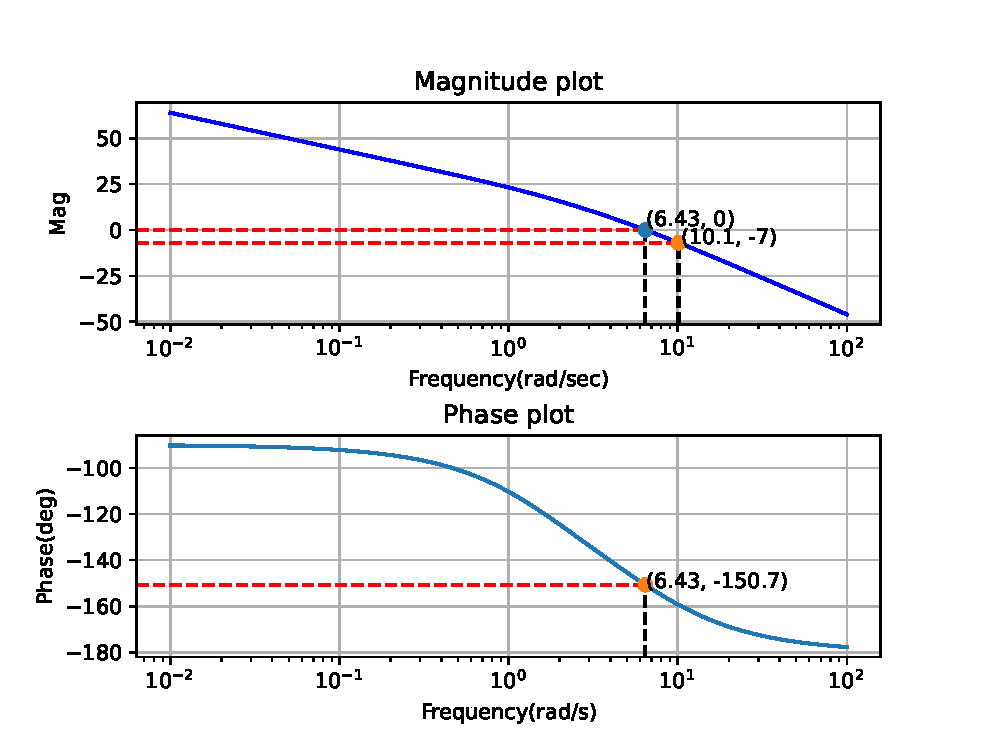
\includegraphics[width=\columnwidth]{./figs/ee18btech11047/ee18btech11047_2.eps}
\caption{1}
\label{fig:ee18btech11047_2}
\end{figure}
The phase margin is 
\begin{align}
\phi_{M} &= 180\degree-150.7\degree \implies \phi_{M} = 29.3\degree \label{eq:ee18btech11047_ph}
\end{align}
The closed-loop bandwith, $\omega_{BW}$(-3 dB frequency), equals the frequency at which the open-loop magnitude response is around -7 dB.
\begin{align}
\omega_{BW} = 10.1  rad/sec \label{eq:ee18btech11047_bw}
\end{align}
\textbf{Damping ratio:} \\
Substitute $\phi_{M}$ value from equation(\ref{eq:ee18btech11047_ph})
\begin{align}
\phi_{M} &= {tan}^{-1}\brak{\frac{2\zeta}{\sqrt{-2\zeta^{2}+\sqrt{1+4\zeta^{2}}}}}\\
\implies \zeta &= 0.34
\end{align}
\textbf{Settling time:} \\
Substitute $\omega_{BW}$ value from equation(\ref{eq:ee18btech11047_bw}) and $\zeta$
\begin{align}
T_{s}&= \frac{4}{\omega_{BW}\zeta}\sqrt{(1-2\zeta^2)+\sqrt{4\zeta^4-4\zeta^2+2}}\\
\implies T_{s} &= 1.65 sec   \\
\end{align}
\textbf{Peak time:}
\begin{align}
T_{p} &= \frac{\pi\zeta T_{s}}{4\sqrt{1-\zeta^2}}\\
\implies T_{p} &= 0.325 sec
\end{align}
\textbf{Percent overshoot:}
\begin{align}
\% OS&=100e^{-(\frac{\zeta\pi}{\sqrt{1-\zeta^2}})}\\
\implies \% OS &= 35.1 \%
\end{align}
Note that the answers will be approximate due to the dominant pole approximation.\\
The following code generates the step response of the system.
\begin{lstlisting}
codes/ee18btech11047/ee18btech11047_3.py
\end{lstlisting}
\begin{figure}[!ht]
\centering
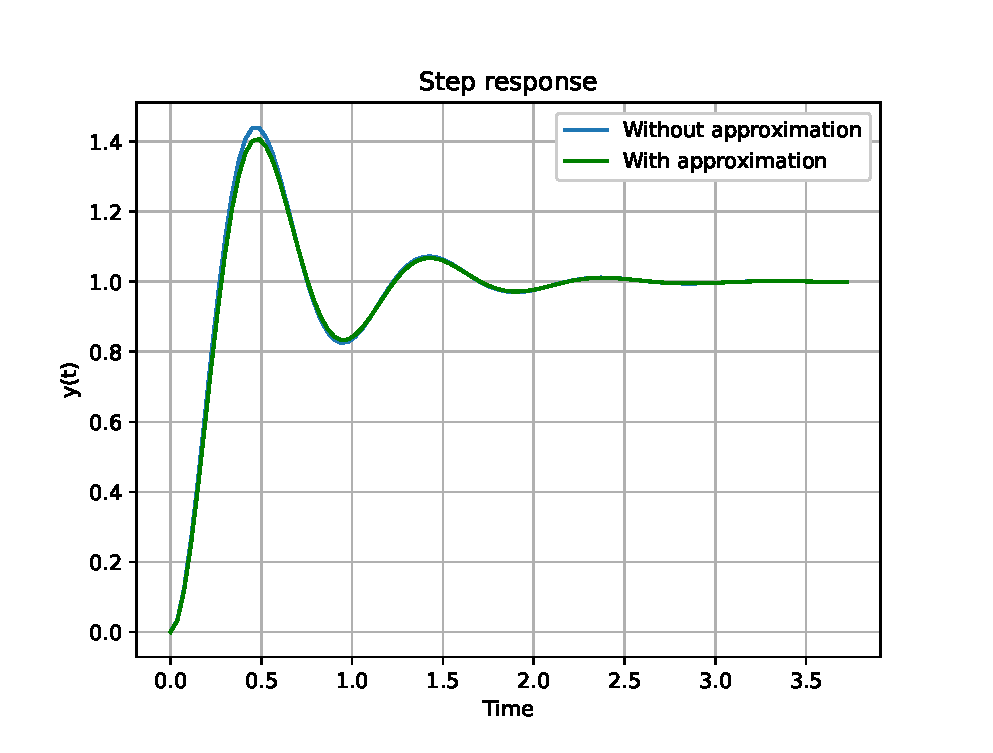
\includegraphics[width=\columnwidth]{./figs/ee18btech11047/ee18btech11047_3.eps}
\caption{2}
\label{fig:ee18btech11047_3}
\end{figure}
\item Find the approximate transfer function for the open loop transfer function
\begin{align}
G(s) &= \frac{75(1+0.2s)}{s(s^{2}+16s+100)}
\end{align}
\solution Using equation \eqref{eq:ee18btech11047_ctf}
\begin{align}
T(s) = \frac{75(1+0.2s)}{s^3 + 16s^2 + 115s +75} 
\end{align}
The following code gives the poles and zeros of the transfer function.
\begin{lstlisting}
codes/ee18btech11047/ee18btech11047_4.py
\end{lstlisting}
\begin{table}[!ht]
\centering
\input{./tables/ee18btech11047/ee18btech11047_2.tex}
\caption{}
\label{table:ee18btech11047_2}
\end{table}
The real part of the complex conjugate poles is comparable with the zero $z_{1}$ of the transfer function.So,they cancel out each other.
The approximated transfer function is of first order.
\begin{align}
T_{2}(s) &= \frac{K_{2}}{(s-p_{1})}\\
T(0) &= T_{2}(s)\\
\implies K_{2} &= p_{1} \\
T_{2}(s) &= \frac{0.72}{s+0.72}
\end{align}
\item Estimate the transient response of the obtained first order system.\\
\solution\\
\textbf{Time constant:}\\
The time constant is the time taken by the step response to rise to 63\% of it's final value.
\begin{align}
T &= \frac{1}{|pole|}\\
T &= \frac{1}{0.72} = 1.388 sec
\end{align}
\textbf{Rise time:}\\
Rise time is the time for the waveform to go from 0.1 to 0.9 of it's final value.
\begin{align}
T_{r} &= \frac{2.2}{|pole|}\\
T_{r} &= \frac{2.2}{0.72} = 3.05 sec
\end{align}
\textbf{Settling time:}\\
Settling time is defined as the time for the response to reach and stay within, 2\% of its final value.
\begin{align}
T_{s} &= \frac{4}{|pole|}\\
T_{s} &= \frac{4}{0.72}=5.55 sec
\end{align}
The following code plots the step response of the system.
\begin{lstlisting}
codes/ee18btech11047/ee18btech11047_5.py
\end{lstlisting}
\begin{figure}[!ht]
\centering
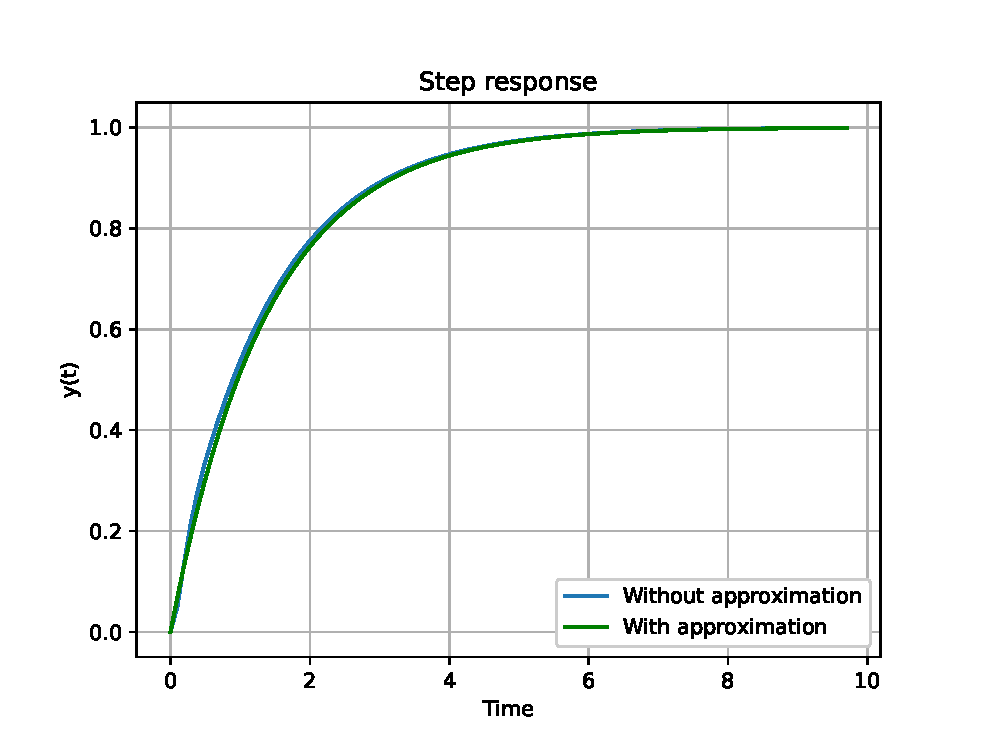
\includegraphics[width=\columnwidth]{./figs/ee18btech11047/ee18btech11047_4.eps}
\caption{}
\label{fig:ee18btech11047_4}
\end{figure}
\end{enumerate}

\caption{}
\label{table:ee18btech11047}
\end{table}
The real poles \brak{p_{1},p_{2}} and zeros \brak{z_{1},z_{2}} cancel out each other as mentioned above.So, we are left with the two conjugate poles.\\
The approximated transfer function is 
\begin{align}
T_{1}(s) &= \frac{K_{1}}{(s-p_{3})(s-p_{4})}\\ 
T(0) &= T_{1}(0)\\
\implies K_{1} &= p_{3}p_{4}\\
T_{1}(s) &= \frac{47.09}{s^{2}+3.74s+47.09}
\end{align}
\item Estimate the transient response of the obtained second order system using the respective bode plot.\\
\solution The following code generates the bode plot for open loop transfer function.
\begin{lstlisting}
codes/ee18btech11047/ee18btech11047_2.py
\end{lstlisting}
\begin{figure}[!ht]
\centering
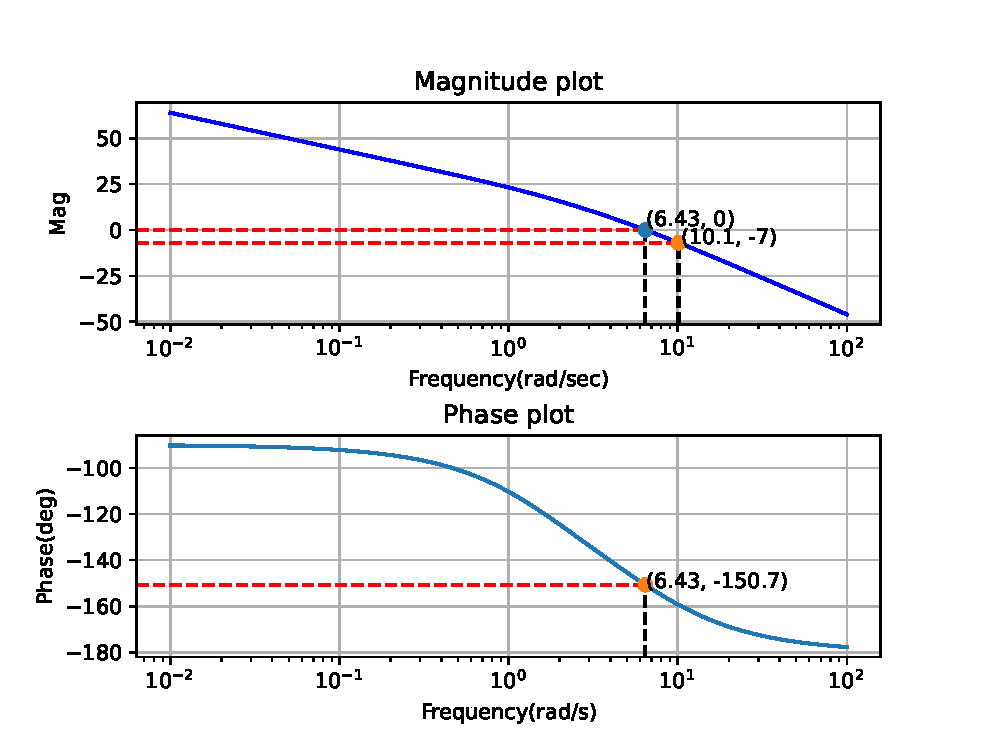
\includegraphics[width=\columnwidth]{./figs/ee18btech11047/ee18btech11047_2.eps}
\caption{1}
\label{fig:ee18btech11047_2}
\end{figure}
The phase margin is 
\begin{align}
\phi_{M} &= 180\degree-150.7\degree \implies \phi_{M} = 29.3\degree \label{eq:ee18btech11047_ph}
\end{align}
The closed-loop bandwith, $\omega_{BW}$(-3 dB frequency), equals the frequency at which the open-loop magnitude response is around -7 dB.
\begin{align}
\omega_{BW} = 10.1  rad/sec \label{eq:ee18btech11047_bw}
\end{align}
\textbf{Damping ratio:} \\
Substitute $\phi_{M}$ value from equation(\ref{eq:ee18btech11047_ph})
\begin{align}
\phi_{M} &= {tan}^{-1}\brak{\frac{2\zeta}{\sqrt{-2\zeta^{2}+\sqrt{1+4\zeta^{2}}}}}\\
\implies \zeta &= 0.34
\end{align}
\textbf{Settling time:} \\
Substitute $\omega_{BW}$ value from equation(\ref{eq:ee18btech11047_bw}) and $\zeta$
\begin{align}
T_{s}&= \frac{4}{\omega_{BW}\zeta}\sqrt{(1-2\zeta^2)+\sqrt{4\zeta^4-4\zeta^2+2}}\\
\implies T_{s} &= 1.65 sec   \\
\end{align}
\textbf{Peak time:}
\begin{align}
T_{p} &= \frac{\pi\zeta T_{s}}{4\sqrt{1-\zeta^2}}\\
\implies T_{p} &= 0.325 sec
\end{align}
\textbf{Percent overshoot:}
\begin{align}
\% OS&=100e^{-(\frac{\zeta\pi}{\sqrt{1-\zeta^2}})}\\
\implies \% OS &= 35.1 \%
\end{align}
Note that the answers will be approximate due to the dominant pole approximation.\\
The following code generates the step response of the system.
\begin{lstlisting}
codes/ee18btech11047/ee18btech11047_3.py
\end{lstlisting}
\begin{figure}[!ht]
\centering
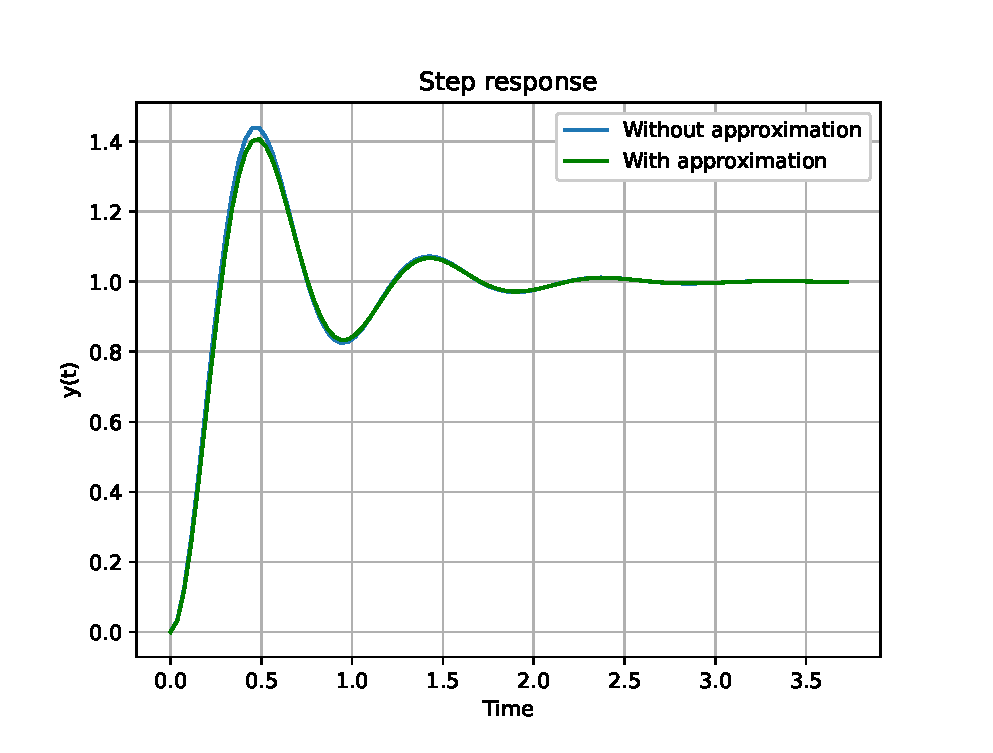
\includegraphics[width=\columnwidth]{./figs/ee18btech11047/ee18btech11047_3.eps}
\caption{2}
\label{fig:ee18btech11047_3}
\end{figure}
\item Find the approximate transfer function for the open loop transfer function
\begin{align}
G(s) &= \frac{75(1+0.2s)}{s(s^{2}+16s+100)}
\end{align}
\solution Using equation \eqref{eq:ee18btech11047_ctf}
\begin{align}
T(s) = \frac{75(1+0.2s)}{s^3 + 16s^2 + 115s +75} 
\end{align}
The following code gives the poles and zeros of the transfer function.
\begin{lstlisting}
codes/ee18btech11047/ee18btech11047_4.py
\end{lstlisting}
\begin{table}[!ht]
\centering
\tikzstyle{block} = [draw, fill=blue!20, rectangle, 
    minimum height=3em, minimum width=6em]
\tikzstyle{sum} = [draw, fill=blue!20, circle, node distance=1cm]
\tikzstyle{input} = [coordinate]
\tikzstyle{output} = [coordinate]
\tikzstyle{pinstyle} = [pin edge={to-,thin,black}]

\begin{tikzpicture}[auto, node distance=2cm,>=latex']
    \node [input, name=input] {};
    \node [sum, right of=input] (sum) {};
    \node [block, right of=sum] (controller) {$G$};
    \node [output, right of=controller] (output) {};
    \node [block, below of=controller] (feedback) {$H$};
    \draw [draw,->] (input) -- node {} (sum);
    \draw [->] (sum) -- node {$V_i$} (controller);
    \draw [->] (controller) -- node [name=y] {$V_o$}(output);
    \draw [->] (y) |- (feedback);
    \draw [->] (feedback) -| node[pos=0.99]{$+$}  node [near end] {$V_f$} (sum);
\end{tikzpicture}

\caption{}
\label{table:ee18btech11047_2}
\end{table}
The real part of the complex conjugate poles is comparable with the zero $z_{1}$ of the transfer function.So,they cancel out each other.
The approximated transfer function is of first order.
\begin{align}
T_{2}(s) &= \frac{K_{2}}{(s-p_{1})}\\
T(0) &= T_{2}(s)\\
\implies K_{2} &= p_{1} \\
T_{2}(s) &= \frac{0.72}{s+0.72}
\end{align}
\item Estimate the transient response of the obtained first order system.\\
\solution\\
\textbf{Time constant:}\\
The time constant is the time taken by the step response to rise to 63\% of it's final value.
\begin{align}
T &= \frac{1}{|pole|}\\
T &= \frac{1}{0.72} = 1.388 sec
\end{align}
\textbf{Rise time:}\\
Rise time is the time for the waveform to go from 0.1 to 0.9 of it's final value.
\begin{align}
T_{r} &= \frac{2.2}{|pole|}\\
T_{r} &= \frac{2.2}{0.72} = 3.05 sec
\end{align}
\textbf{Settling time:}\\
Settling time is defined as the time for the response to reach and stay within, 2\% of its final value.
\begin{align}
T_{s} &= \frac{4}{|pole|}\\
T_{s} &= \frac{4}{0.72}=5.55 sec
\end{align}
The following code plots the step response of the system.
\begin{lstlisting}
codes/ee18btech11047/ee18btech11047_5.py
\end{lstlisting}
\begin{figure}[!ht]
\centering
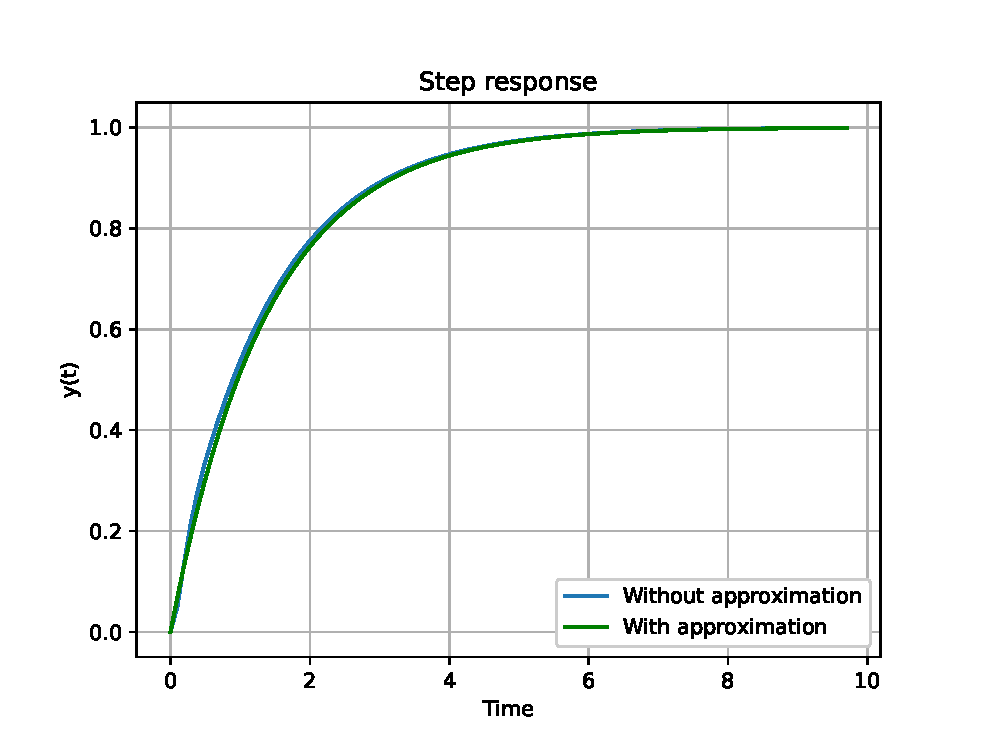
\includegraphics[width=\columnwidth]{./figs/ee18btech11047/ee18btech11047_4.eps}
\caption{}
\label{fig:ee18btech11047_4}
\end{figure}
\end{enumerate}
}
	\end{center}
\caption{}
\label{fig:ee18btech11047}
\end{figure}

\item Find the approximate transfer function for the open loop transfer function.
\begin{align}
G(s) &= \frac{50(s+3)(s+5)}{s(s+2)(s+4)(s+6)}
\end{align}
\solution Using equation\eqref{eq:ee18btech11047_ctf}
\begin{align}
T(s) &= \frac{50(s^{2}+8s+15)}{s^4+12s^3+94s^2+448s+750}
\end{align}
The following code gives the poles and zeros of the transfer function.
\begin{lstlisting}
codes/ee18btech11047/ee18btech11047_1.py
\end{lstlisting}
\begin{table}[!ht]
\centering
\begin{enumerate}[label=\thesubsection.\arabic*.,ref=\thesubsection.\theenumi]
\numberwithin{equation}{enumi}

\item Consider the following transfer functions as open-loop transfer functions in two different unity feedback(negative) systems.
\begin{align}
G(s) &= \frac{50(s+3)(s+5)}{s(s+2)(s+4)(s+6)} 
\\
G(s) &= \frac{75(1+0.2s)}{s(s^{2}+16s+100)} 
\end{align}
Estimate transient response of these systems from their respective bode plots.
\\
\solution 
\begin{enumerate}
\item  The dominant pole approximation is used to characterize higher order systems because it is difficult to characterize and analyse systems with order greater than 3.
\item Consider a transfer function.
\begin{align}
H(s) = K\frac{\alpha\beta}{(s+\alpha)(s+\beta)}
\end{align}
It has two poles $-\alpha$ and $-\beta $. If the magnitude of $\beta$ is very large compared to $\alpha$ (typically if $\frac{|\beta|}{|\alpha|}$ $>$ 5  ) we can approximate for the transfer function assuming $s$ is sufficiently small compared to $\beta$ as follows.
\begin{align}
H(s) = K_{2}\brak{\frac{1}{s+\alpha}}
\end{align}
Note that the value of $H(0)$ should be unchanged for the exact and approximate transfer functions.This is necessary to ensure that the final value of the step response is unchanged.
\begin{align}
\lim_{t\to\infty} y(t) &= \lim_{s\to 0} sY(s) \\
\lim_{t\to\infty} y(t) &= \lim_{s\to 0} sU(s)H(s) = H(0)
\end{align}
In order to acheive this we adjust the gain value of the approximated transfer function by equating $H(0)$ values.
\begin{align}
\implies H(s) = K\frac{\alpha}{(s+\alpha)}
\end{align}
\item In terms of poles, the pole closer to the origin is considered as the dominating pole.As considered above,the magnitude of $\alpha$ is small therefore the time constant $\frac{1}{\alpha}$ will be high and reaches equilibrium slowly and vice versa in case of  $\beta$.Therefore,this approximation assumes that the slowest part of the system dominates the response.The faster parts of the system are ignored.
\item Complex poles along with real poles : In this case the dominant pole(s) can be determined by comparing only the real parts.If the real part of the complex conjugate poles is greater in magnitude than the real pole, the two complex conjugate poles the dominant poles.
\item If the transfer function has zeros along with poles,we have to consider the fact that pole and zero cancel out each other if their respective magnitudes are comparable.
\end{enumerate}
\item Find the closed loop transfer function of a negative unity feedback system given open loop transfer function $G(s)$ .\\
\solution 
\begin{align}
\label{eq:ee18btech11047_ctf}
T(s) &= \frac{G(s)}{1+G(s)}
\end{align}
\begin{figure}[!ht]
	\begin{center}
		\resizebox{\columnwidth}{!}{\begin{enumerate}[label=\thesubsection.\arabic*.,ref=\thesubsection.\theenumi]
\numberwithin{equation}{enumi}

\item Consider the following transfer functions as open-loop transfer functions in two different unity feedback(negative) systems.
\begin{align}
G(s) &= \frac{50(s+3)(s+5)}{s(s+2)(s+4)(s+6)} 
\\
G(s) &= \frac{75(1+0.2s)}{s(s^{2}+16s+100)} 
\end{align}
Estimate transient response of these systems from their respective bode plots.
\\
\solution 
\begin{enumerate}
\item  The dominant pole approximation is used to characterize higher order systems because it is difficult to characterize and analyse systems with order greater than 3.
\item Consider a transfer function.
\begin{align}
H(s) = K\frac{\alpha\beta}{(s+\alpha)(s+\beta)}
\end{align}
It has two poles $-\alpha$ and $-\beta $. If the magnitude of $\beta$ is very large compared to $\alpha$ (typically if $\frac{|\beta|}{|\alpha|}$ $>$ 5  ) we can approximate for the transfer function assuming $s$ is sufficiently small compared to $\beta$ as follows.
\begin{align}
H(s) = K_{2}\brak{\frac{1}{s+\alpha}}
\end{align}
Note that the value of $H(0)$ should be unchanged for the exact and approximate transfer functions.This is necessary to ensure that the final value of the step response is unchanged.
\begin{align}
\lim_{t\to\infty} y(t) &= \lim_{s\to 0} sY(s) \\
\lim_{t\to\infty} y(t) &= \lim_{s\to 0} sU(s)H(s) = H(0)
\end{align}
In order to acheive this we adjust the gain value of the approximated transfer function by equating $H(0)$ values.
\begin{align}
\implies H(s) = K\frac{\alpha}{(s+\alpha)}
\end{align}
\item In terms of poles, the pole closer to the origin is considered as the dominating pole.As considered above,the magnitude of $\alpha$ is small therefore the time constant $\frac{1}{\alpha}$ will be high and reaches equilibrium slowly and vice versa in case of  $\beta$.Therefore,this approximation assumes that the slowest part of the system dominates the response.The faster parts of the system are ignored.
\item Complex poles along with real poles : In this case the dominant pole(s) can be determined by comparing only the real parts.If the real part of the complex conjugate poles is greater in magnitude than the real pole, the two complex conjugate poles the dominant poles.
\item If the transfer function has zeros along with poles,we have to consider the fact that pole and zero cancel out each other if their respective magnitudes are comparable.
\end{enumerate}
\item Find the closed loop transfer function of a negative unity feedback system given open loop transfer function $G(s)$ .\\
\solution 
\begin{align}
\label{eq:ee18btech11047_ctf}
T(s) &= \frac{G(s)}{1+G(s)}
\end{align}
\begin{figure}[!ht]
	\begin{center}
		\resizebox{\columnwidth}{!}{\input{./figs/ee18btech11047/ee18btech11047.tex}}
	\end{center}
\caption{}
\label{fig:ee18btech11047}
\end{figure}

\item Find the approximate transfer function for the open loop transfer function.
\begin{align}
G(s) &= \frac{50(s+3)(s+5)}{s(s+2)(s+4)(s+6)}
\end{align}
\solution Using equation\eqref{eq:ee18btech11047_ctf}
\begin{align}
T(s) &= \frac{50(s^{2}+8s+15)}{s^4+12s^3+94s^2+448s+750}
\end{align}
The following code gives the poles and zeros of the transfer function.
\begin{lstlisting}
codes/ee18btech11047/ee18btech11047_1.py
\end{lstlisting}
\begin{table}[!ht]
\centering
\input{./tables/ee18btech11047/ee18btech11047.tex}
\caption{}
\label{table:ee18btech11047}
\end{table}
The real poles \brak{p_{1},p_{2}} and zeros \brak{z_{1},z_{2}} cancel out each other as mentioned above.So, we are left with the two conjugate poles.\\
The approximated transfer function is 
\begin{align}
T_{1}(s) &= \frac{K_{1}}{(s-p_{3})(s-p_{4})}\\ 
T(0) &= T_{1}(0)\\
\implies K_{1} &= p_{3}p_{4}\\
T_{1}(s) &= \frac{47.09}{s^{2}+3.74s+47.09}
\end{align}
\item Estimate the transient response of the obtained second order system using the respective bode plot.\\
\solution The following code generates the bode plot for open loop transfer function.
\begin{lstlisting}
codes/ee18btech11047/ee18btech11047_2.py
\end{lstlisting}
\begin{figure}[!ht]
\centering
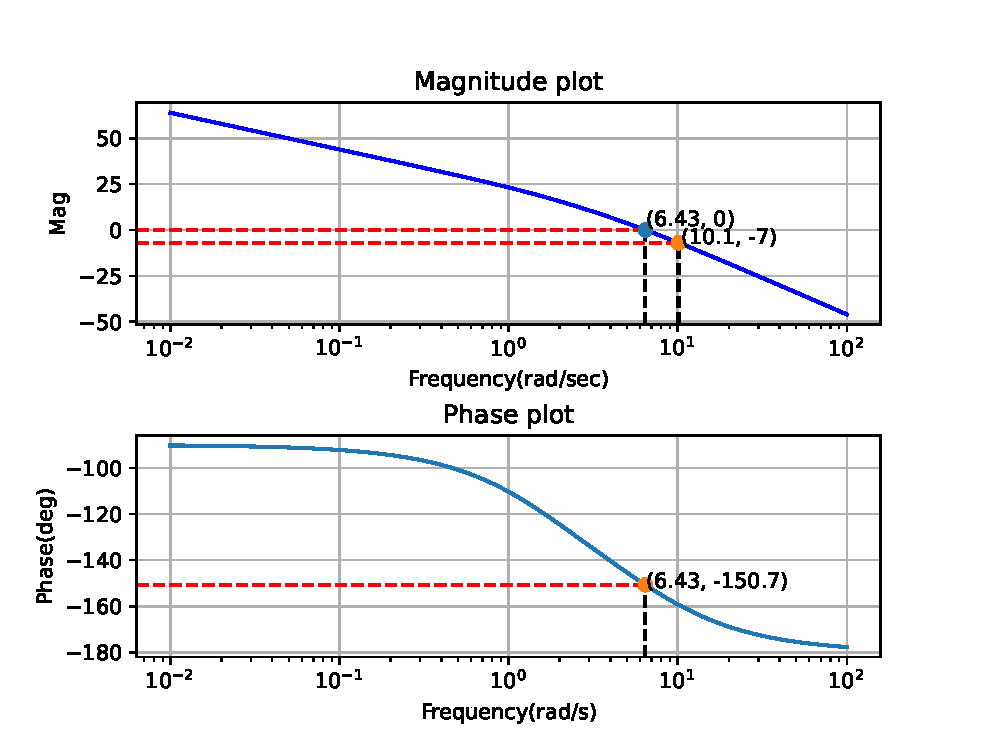
\includegraphics[width=\columnwidth]{./figs/ee18btech11047/ee18btech11047_2.eps}
\caption{1}
\label{fig:ee18btech11047_2}
\end{figure}
The phase margin is 
\begin{align}
\phi_{M} &= 180\degree-150.7\degree \implies \phi_{M} = 29.3\degree \label{eq:ee18btech11047_ph}
\end{align}
The closed-loop bandwith, $\omega_{BW}$(-3 dB frequency), equals the frequency at which the open-loop magnitude response is around -7 dB.
\begin{align}
\omega_{BW} = 10.1  rad/sec \label{eq:ee18btech11047_bw}
\end{align}
\textbf{Damping ratio:} \\
Substitute $\phi_{M}$ value from equation(\ref{eq:ee18btech11047_ph})
\begin{align}
\phi_{M} &= {tan}^{-1}\brak{\frac{2\zeta}{\sqrt{-2\zeta^{2}+\sqrt{1+4\zeta^{2}}}}}\\
\implies \zeta &= 0.34
\end{align}
\textbf{Settling time:} \\
Substitute $\omega_{BW}$ value from equation(\ref{eq:ee18btech11047_bw}) and $\zeta$
\begin{align}
T_{s}&= \frac{4}{\omega_{BW}\zeta}\sqrt{(1-2\zeta^2)+\sqrt{4\zeta^4-4\zeta^2+2}}\\
\implies T_{s} &= 1.65 sec   \\
\end{align}
\textbf{Peak time:}
\begin{align}
T_{p} &= \frac{\pi\zeta T_{s}}{4\sqrt{1-\zeta^2}}\\
\implies T_{p} &= 0.325 sec
\end{align}
\textbf{Percent overshoot:}
\begin{align}
\% OS&=100e^{-(\frac{\zeta\pi}{\sqrt{1-\zeta^2}})}\\
\implies \% OS &= 35.1 \%
\end{align}
Note that the answers will be approximate due to the dominant pole approximation.\\
The following code generates the step response of the system.
\begin{lstlisting}
codes/ee18btech11047/ee18btech11047_3.py
\end{lstlisting}
\begin{figure}[!ht]
\centering
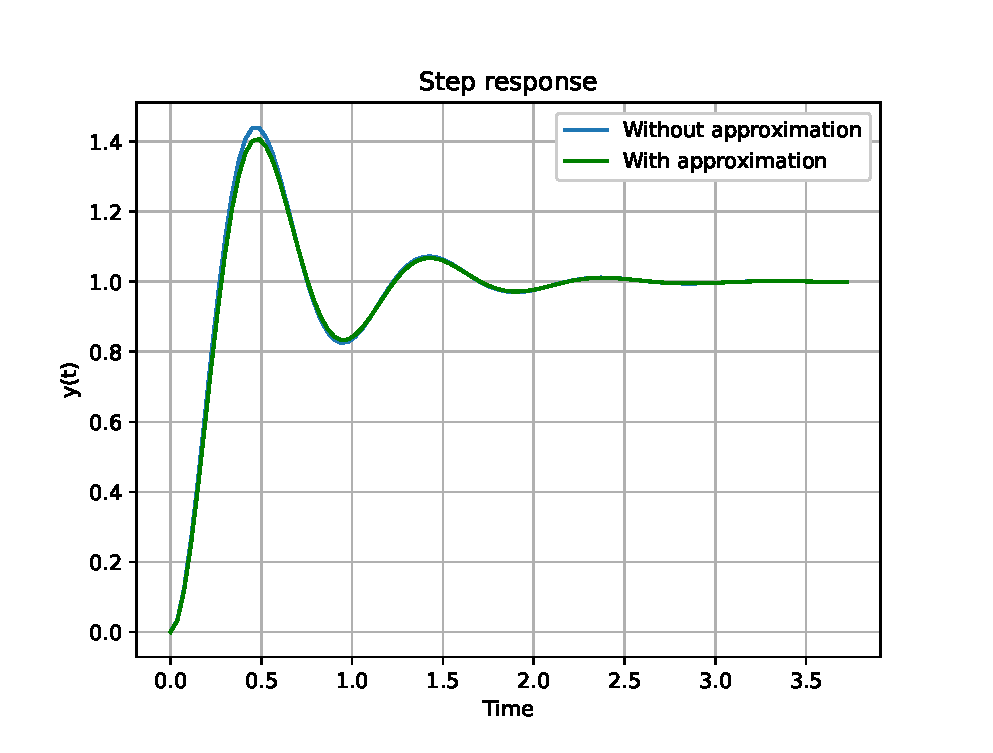
\includegraphics[width=\columnwidth]{./figs/ee18btech11047/ee18btech11047_3.eps}
\caption{2}
\label{fig:ee18btech11047_3}
\end{figure}
\item Find the approximate transfer function for the open loop transfer function
\begin{align}
G(s) &= \frac{75(1+0.2s)}{s(s^{2}+16s+100)}
\end{align}
\solution Using equation \eqref{eq:ee18btech11047_ctf}
\begin{align}
T(s) = \frac{75(1+0.2s)}{s^3 + 16s^2 + 115s +75} 
\end{align}
The following code gives the poles and zeros of the transfer function.
\begin{lstlisting}
codes/ee18btech11047/ee18btech11047_4.py
\end{lstlisting}
\begin{table}[!ht]
\centering
\input{./tables/ee18btech11047/ee18btech11047_2.tex}
\caption{}
\label{table:ee18btech11047_2}
\end{table}
The real part of the complex conjugate poles is comparable with the zero $z_{1}$ of the transfer function.So,they cancel out each other.
The approximated transfer function is of first order.
\begin{align}
T_{2}(s) &= \frac{K_{2}}{(s-p_{1})}\\
T(0) &= T_{2}(s)\\
\implies K_{2} &= p_{1} \\
T_{2}(s) &= \frac{0.72}{s+0.72}
\end{align}
\item Estimate the transient response of the obtained first order system.\\
\solution\\
\textbf{Time constant:}\\
The time constant is the time taken by the step response to rise to 63\% of it's final value.
\begin{align}
T &= \frac{1}{|pole|}\\
T &= \frac{1}{0.72} = 1.388 sec
\end{align}
\textbf{Rise time:}\\
Rise time is the time for the waveform to go from 0.1 to 0.9 of it's final value.
\begin{align}
T_{r} &= \frac{2.2}{|pole|}\\
T_{r} &= \frac{2.2}{0.72} = 3.05 sec
\end{align}
\textbf{Settling time:}\\
Settling time is defined as the time for the response to reach and stay within, 2\% of its final value.
\begin{align}
T_{s} &= \frac{4}{|pole|}\\
T_{s} &= \frac{4}{0.72}=5.55 sec
\end{align}
The following code plots the step response of the system.
\begin{lstlisting}
codes/ee18btech11047/ee18btech11047_5.py
\end{lstlisting}
\begin{figure}[!ht]
\centering
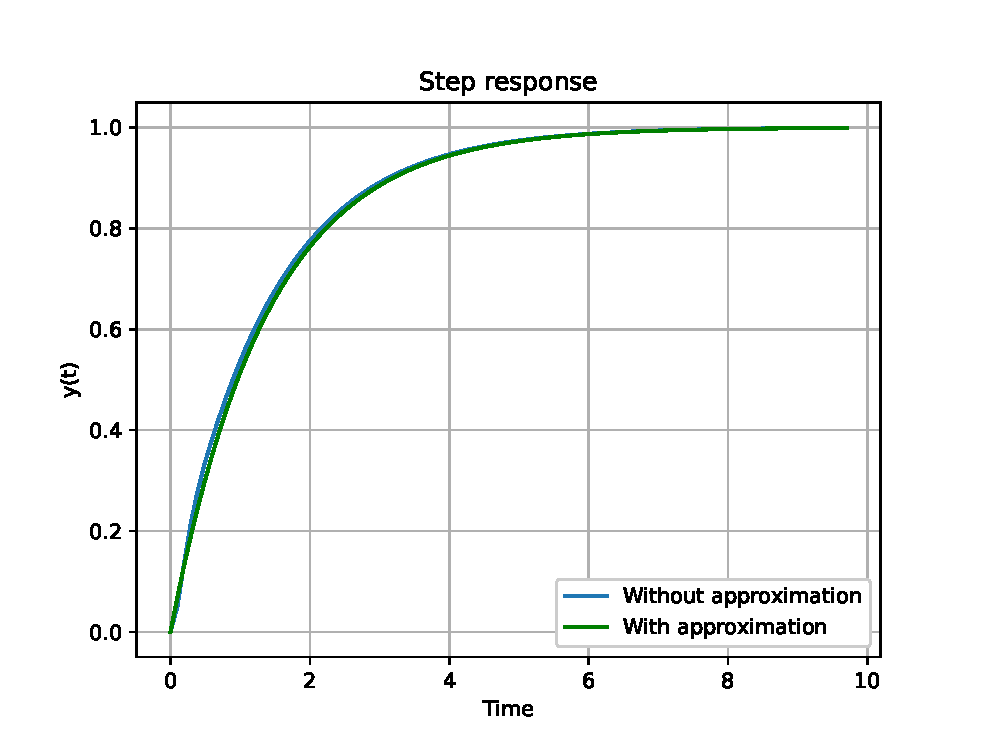
\includegraphics[width=\columnwidth]{./figs/ee18btech11047/ee18btech11047_4.eps}
\caption{}
\label{fig:ee18btech11047_4}
\end{figure}
\end{enumerate}
}
	\end{center}
\caption{}
\label{fig:ee18btech11047}
\end{figure}

\item Find the approximate transfer function for the open loop transfer function.
\begin{align}
G(s) &= \frac{50(s+3)(s+5)}{s(s+2)(s+4)(s+6)}
\end{align}
\solution Using equation\eqref{eq:ee18btech11047_ctf}
\begin{align}
T(s) &= \frac{50(s^{2}+8s+15)}{s^4+12s^3+94s^2+448s+750}
\end{align}
The following code gives the poles and zeros of the transfer function.
\begin{lstlisting}
codes/ee18btech11047/ee18btech11047_1.py
\end{lstlisting}
\begin{table}[!ht]
\centering
\begin{enumerate}[label=\thesubsection.\arabic*.,ref=\thesubsection.\theenumi]
\numberwithin{equation}{enumi}

\item Consider the following transfer functions as open-loop transfer functions in two different unity feedback(negative) systems.
\begin{align}
G(s) &= \frac{50(s+3)(s+5)}{s(s+2)(s+4)(s+6)} 
\\
G(s) &= \frac{75(1+0.2s)}{s(s^{2}+16s+100)} 
\end{align}
Estimate transient response of these systems from their respective bode plots.
\\
\solution 
\begin{enumerate}
\item  The dominant pole approximation is used to characterize higher order systems because it is difficult to characterize and analyse systems with order greater than 3.
\item Consider a transfer function.
\begin{align}
H(s) = K\frac{\alpha\beta}{(s+\alpha)(s+\beta)}
\end{align}
It has two poles $-\alpha$ and $-\beta $. If the magnitude of $\beta$ is very large compared to $\alpha$ (typically if $\frac{|\beta|}{|\alpha|}$ $>$ 5  ) we can approximate for the transfer function assuming $s$ is sufficiently small compared to $\beta$ as follows.
\begin{align}
H(s) = K_{2}\brak{\frac{1}{s+\alpha}}
\end{align}
Note that the value of $H(0)$ should be unchanged for the exact and approximate transfer functions.This is necessary to ensure that the final value of the step response is unchanged.
\begin{align}
\lim_{t\to\infty} y(t) &= \lim_{s\to 0} sY(s) \\
\lim_{t\to\infty} y(t) &= \lim_{s\to 0} sU(s)H(s) = H(0)
\end{align}
In order to acheive this we adjust the gain value of the approximated transfer function by equating $H(0)$ values.
\begin{align}
\implies H(s) = K\frac{\alpha}{(s+\alpha)}
\end{align}
\item In terms of poles, the pole closer to the origin is considered as the dominating pole.As considered above,the magnitude of $\alpha$ is small therefore the time constant $\frac{1}{\alpha}$ will be high and reaches equilibrium slowly and vice versa in case of  $\beta$.Therefore,this approximation assumes that the slowest part of the system dominates the response.The faster parts of the system are ignored.
\item Complex poles along with real poles : In this case the dominant pole(s) can be determined by comparing only the real parts.If the real part of the complex conjugate poles is greater in magnitude than the real pole, the two complex conjugate poles the dominant poles.
\item If the transfer function has zeros along with poles,we have to consider the fact that pole and zero cancel out each other if their respective magnitudes are comparable.
\end{enumerate}
\item Find the closed loop transfer function of a negative unity feedback system given open loop transfer function $G(s)$ .\\
\solution 
\begin{align}
\label{eq:ee18btech11047_ctf}
T(s) &= \frac{G(s)}{1+G(s)}
\end{align}
\begin{figure}[!ht]
	\begin{center}
		\resizebox{\columnwidth}{!}{\input{./figs/ee18btech11047/ee18btech11047.tex}}
	\end{center}
\caption{}
\label{fig:ee18btech11047}
\end{figure}

\item Find the approximate transfer function for the open loop transfer function.
\begin{align}
G(s) &= \frac{50(s+3)(s+5)}{s(s+2)(s+4)(s+6)}
\end{align}
\solution Using equation\eqref{eq:ee18btech11047_ctf}
\begin{align}
T(s) &= \frac{50(s^{2}+8s+15)}{s^4+12s^3+94s^2+448s+750}
\end{align}
The following code gives the poles and zeros of the transfer function.
\begin{lstlisting}
codes/ee18btech11047/ee18btech11047_1.py
\end{lstlisting}
\begin{table}[!ht]
\centering
\input{./tables/ee18btech11047/ee18btech11047.tex}
\caption{}
\label{table:ee18btech11047}
\end{table}
The real poles \brak{p_{1},p_{2}} and zeros \brak{z_{1},z_{2}} cancel out each other as mentioned above.So, we are left with the two conjugate poles.\\
The approximated transfer function is 
\begin{align}
T_{1}(s) &= \frac{K_{1}}{(s-p_{3})(s-p_{4})}\\ 
T(0) &= T_{1}(0)\\
\implies K_{1} &= p_{3}p_{4}\\
T_{1}(s) &= \frac{47.09}{s^{2}+3.74s+47.09}
\end{align}
\item Estimate the transient response of the obtained second order system using the respective bode plot.\\
\solution The following code generates the bode plot for open loop transfer function.
\begin{lstlisting}
codes/ee18btech11047/ee18btech11047_2.py
\end{lstlisting}
\begin{figure}[!ht]
\centering
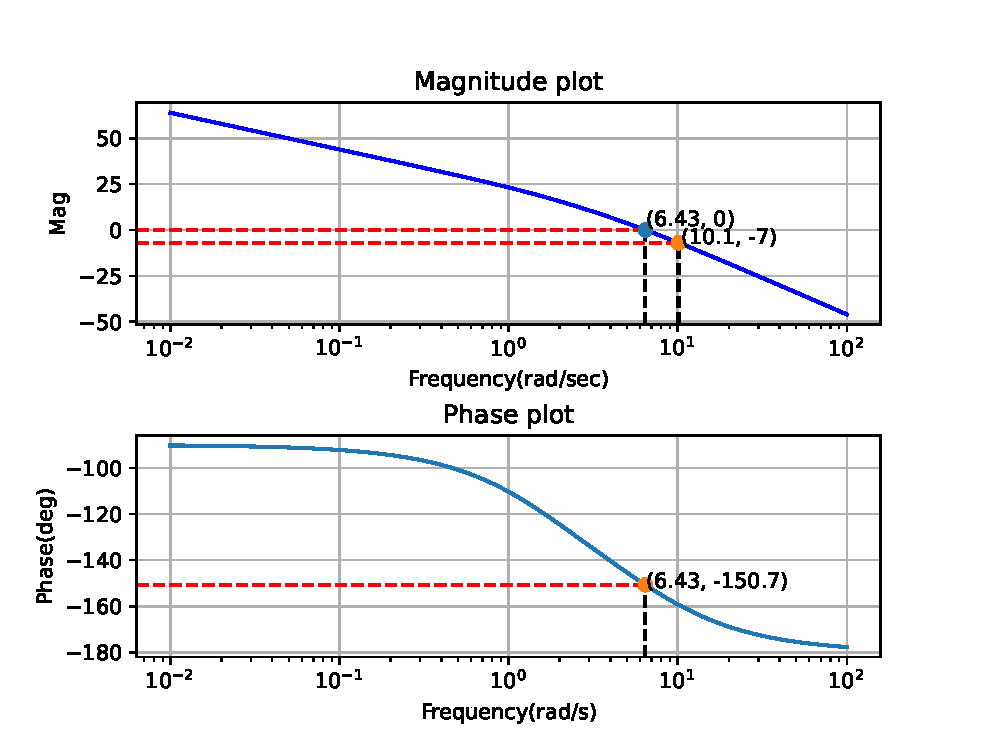
\includegraphics[width=\columnwidth]{./figs/ee18btech11047/ee18btech11047_2.eps}
\caption{1}
\label{fig:ee18btech11047_2}
\end{figure}
The phase margin is 
\begin{align}
\phi_{M} &= 180\degree-150.7\degree \implies \phi_{M} = 29.3\degree \label{eq:ee18btech11047_ph}
\end{align}
The closed-loop bandwith, $\omega_{BW}$(-3 dB frequency), equals the frequency at which the open-loop magnitude response is around -7 dB.
\begin{align}
\omega_{BW} = 10.1  rad/sec \label{eq:ee18btech11047_bw}
\end{align}
\textbf{Damping ratio:} \\
Substitute $\phi_{M}$ value from equation(\ref{eq:ee18btech11047_ph})
\begin{align}
\phi_{M} &= {tan}^{-1}\brak{\frac{2\zeta}{\sqrt{-2\zeta^{2}+\sqrt{1+4\zeta^{2}}}}}\\
\implies \zeta &= 0.34
\end{align}
\textbf{Settling time:} \\
Substitute $\omega_{BW}$ value from equation(\ref{eq:ee18btech11047_bw}) and $\zeta$
\begin{align}
T_{s}&= \frac{4}{\omega_{BW}\zeta}\sqrt{(1-2\zeta^2)+\sqrt{4\zeta^4-4\zeta^2+2}}\\
\implies T_{s} &= 1.65 sec   \\
\end{align}
\textbf{Peak time:}
\begin{align}
T_{p} &= \frac{\pi\zeta T_{s}}{4\sqrt{1-\zeta^2}}\\
\implies T_{p} &= 0.325 sec
\end{align}
\textbf{Percent overshoot:}
\begin{align}
\% OS&=100e^{-(\frac{\zeta\pi}{\sqrt{1-\zeta^2}})}\\
\implies \% OS &= 35.1 \%
\end{align}
Note that the answers will be approximate due to the dominant pole approximation.\\
The following code generates the step response of the system.
\begin{lstlisting}
codes/ee18btech11047/ee18btech11047_3.py
\end{lstlisting}
\begin{figure}[!ht]
\centering
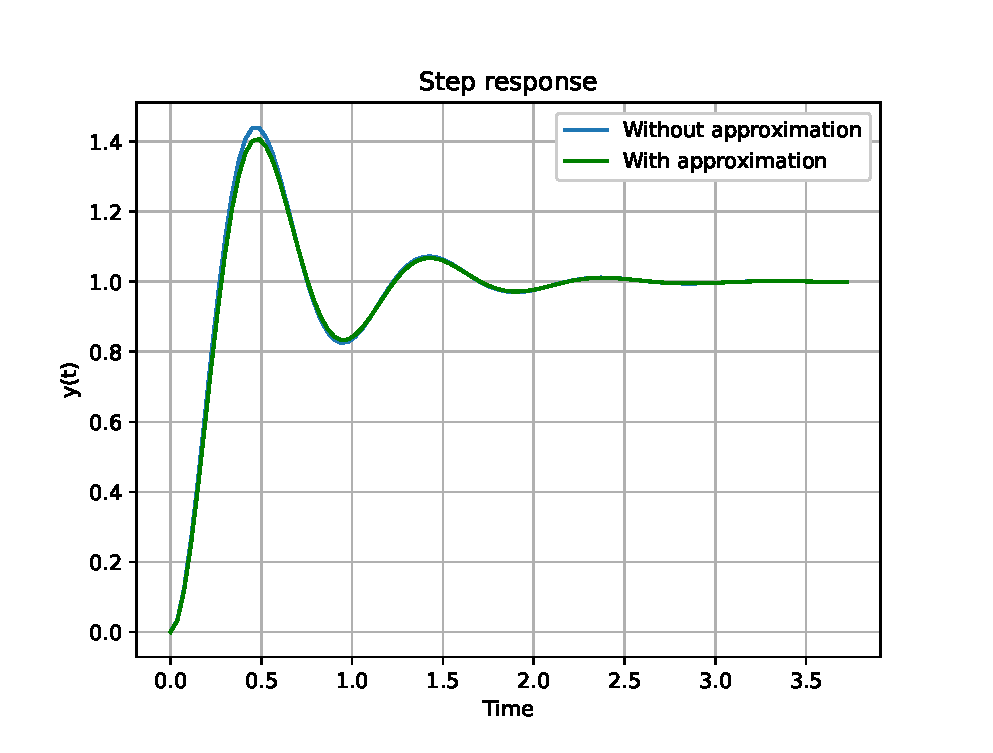
\includegraphics[width=\columnwidth]{./figs/ee18btech11047/ee18btech11047_3.eps}
\caption{2}
\label{fig:ee18btech11047_3}
\end{figure}
\item Find the approximate transfer function for the open loop transfer function
\begin{align}
G(s) &= \frac{75(1+0.2s)}{s(s^{2}+16s+100)}
\end{align}
\solution Using equation \eqref{eq:ee18btech11047_ctf}
\begin{align}
T(s) = \frac{75(1+0.2s)}{s^3 + 16s^2 + 115s +75} 
\end{align}
The following code gives the poles and zeros of the transfer function.
\begin{lstlisting}
codes/ee18btech11047/ee18btech11047_4.py
\end{lstlisting}
\begin{table}[!ht]
\centering
\input{./tables/ee18btech11047/ee18btech11047_2.tex}
\caption{}
\label{table:ee18btech11047_2}
\end{table}
The real part of the complex conjugate poles is comparable with the zero $z_{1}$ of the transfer function.So,they cancel out each other.
The approximated transfer function is of first order.
\begin{align}
T_{2}(s) &= \frac{K_{2}}{(s-p_{1})}\\
T(0) &= T_{2}(s)\\
\implies K_{2} &= p_{1} \\
T_{2}(s) &= \frac{0.72}{s+0.72}
\end{align}
\item Estimate the transient response of the obtained first order system.\\
\solution\\
\textbf{Time constant:}\\
The time constant is the time taken by the step response to rise to 63\% of it's final value.
\begin{align}
T &= \frac{1}{|pole|}\\
T &= \frac{1}{0.72} = 1.388 sec
\end{align}
\textbf{Rise time:}\\
Rise time is the time for the waveform to go from 0.1 to 0.9 of it's final value.
\begin{align}
T_{r} &= \frac{2.2}{|pole|}\\
T_{r} &= \frac{2.2}{0.72} = 3.05 sec
\end{align}
\textbf{Settling time:}\\
Settling time is defined as the time for the response to reach and stay within, 2\% of its final value.
\begin{align}
T_{s} &= \frac{4}{|pole|}\\
T_{s} &= \frac{4}{0.72}=5.55 sec
\end{align}
The following code plots the step response of the system.
\begin{lstlisting}
codes/ee18btech11047/ee18btech11047_5.py
\end{lstlisting}
\begin{figure}[!ht]
\centering
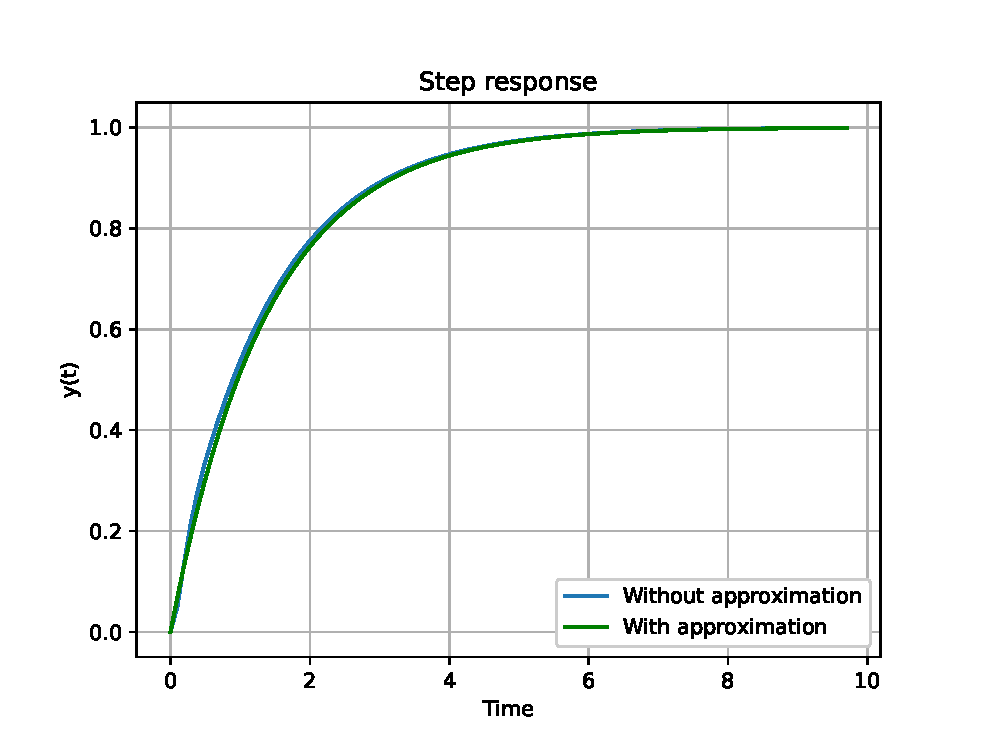
\includegraphics[width=\columnwidth]{./figs/ee18btech11047/ee18btech11047_4.eps}
\caption{}
\label{fig:ee18btech11047_4}
\end{figure}
\end{enumerate}

\caption{}
\label{table:ee18btech11047}
\end{table}
The real poles \brak{p_{1},p_{2}} and zeros \brak{z_{1},z_{2}} cancel out each other as mentioned above.So, we are left with the two conjugate poles.\\
The approximated transfer function is 
\begin{align}
T_{1}(s) &= \frac{K_{1}}{(s-p_{3})(s-p_{4})}\\ 
T(0) &= T_{1}(0)\\
\implies K_{1} &= p_{3}p_{4}\\
T_{1}(s) &= \frac{47.09}{s^{2}+3.74s+47.09}
\end{align}
\item Estimate the transient response of the obtained second order system using the respective bode plot.\\
\solution The following code generates the bode plot for open loop transfer function.
\begin{lstlisting}
codes/ee18btech11047/ee18btech11047_2.py
\end{lstlisting}
\begin{figure}[!ht]
\centering
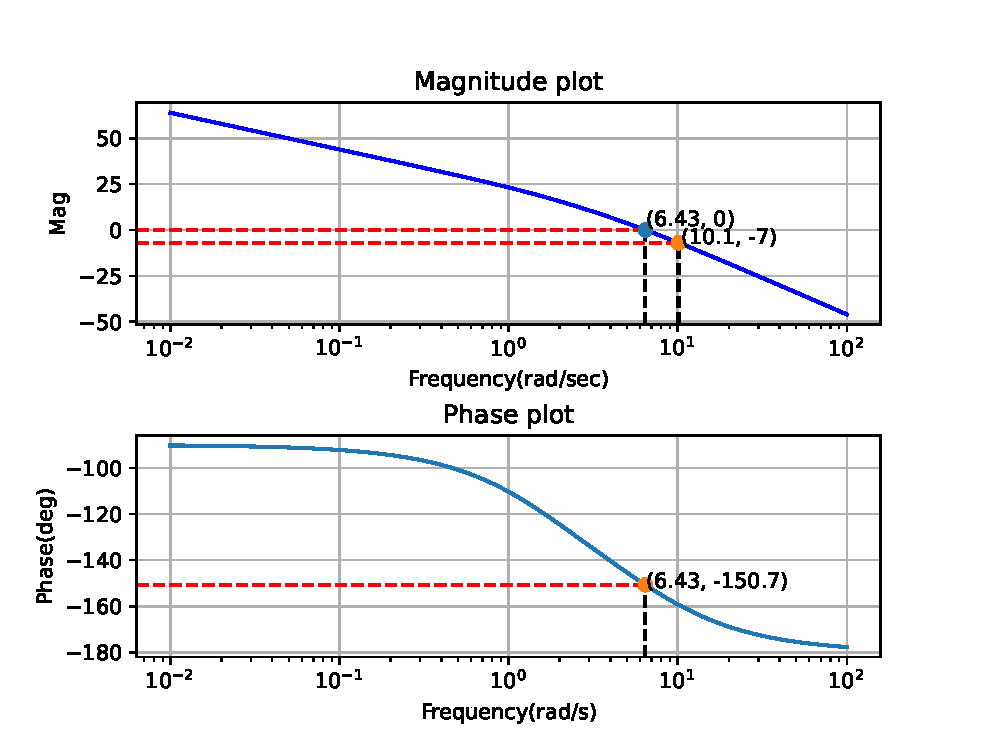
\includegraphics[width=\columnwidth]{./figs/ee18btech11047/ee18btech11047_2.eps}
\caption{1}
\label{fig:ee18btech11047_2}
\end{figure}
The phase margin is 
\begin{align}
\phi_{M} &= 180\degree-150.7\degree \implies \phi_{M} = 29.3\degree \label{eq:ee18btech11047_ph}
\end{align}
The closed-loop bandwith, $\omega_{BW}$(-3 dB frequency), equals the frequency at which the open-loop magnitude response is around -7 dB.
\begin{align}
\omega_{BW} = 10.1  rad/sec \label{eq:ee18btech11047_bw}
\end{align}
\textbf{Damping ratio:} \\
Substitute $\phi_{M}$ value from equation(\ref{eq:ee18btech11047_ph})
\begin{align}
\phi_{M} &= {tan}^{-1}\brak{\frac{2\zeta}{\sqrt{-2\zeta^{2}+\sqrt{1+4\zeta^{2}}}}}\\
\implies \zeta &= 0.34
\end{align}
\textbf{Settling time:} \\
Substitute $\omega_{BW}$ value from equation(\ref{eq:ee18btech11047_bw}) and $\zeta$
\begin{align}
T_{s}&= \frac{4}{\omega_{BW}\zeta}\sqrt{(1-2\zeta^2)+\sqrt{4\zeta^4-4\zeta^2+2}}\\
\implies T_{s} &= 1.65 sec   \\
\end{align}
\textbf{Peak time:}
\begin{align}
T_{p} &= \frac{\pi\zeta T_{s}}{4\sqrt{1-\zeta^2}}\\
\implies T_{p} &= 0.325 sec
\end{align}
\textbf{Percent overshoot:}
\begin{align}
\% OS&=100e^{-(\frac{\zeta\pi}{\sqrt{1-\zeta^2}})}\\
\implies \% OS &= 35.1 \%
\end{align}
Note that the answers will be approximate due to the dominant pole approximation.\\
The following code generates the step response of the system.
\begin{lstlisting}
codes/ee18btech11047/ee18btech11047_3.py
\end{lstlisting}
\begin{figure}[!ht]
\centering
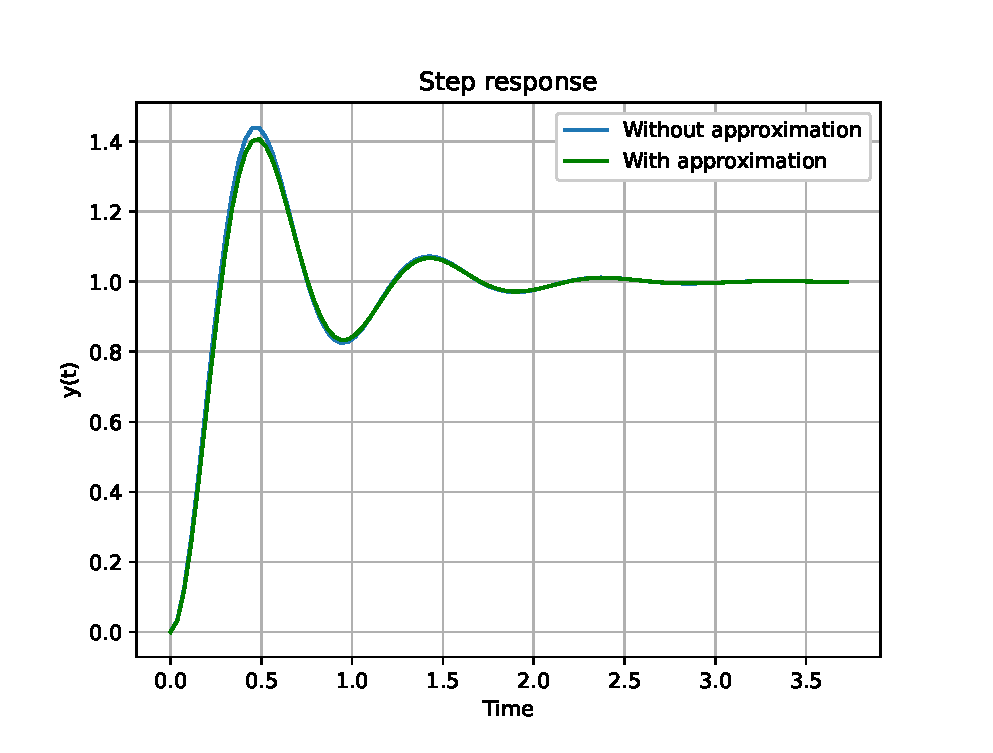
\includegraphics[width=\columnwidth]{./figs/ee18btech11047/ee18btech11047_3.eps}
\caption{2}
\label{fig:ee18btech11047_3}
\end{figure}
\item Find the approximate transfer function for the open loop transfer function
\begin{align}
G(s) &= \frac{75(1+0.2s)}{s(s^{2}+16s+100)}
\end{align}
\solution Using equation \eqref{eq:ee18btech11047_ctf}
\begin{align}
T(s) = \frac{75(1+0.2s)}{s^3 + 16s^2 + 115s +75} 
\end{align}
The following code gives the poles and zeros of the transfer function.
\begin{lstlisting}
codes/ee18btech11047/ee18btech11047_4.py
\end{lstlisting}
\begin{table}[!ht]
\centering
\tikzstyle{block} = [draw, fill=blue!20, rectangle, 
    minimum height=3em, minimum width=6em]
\tikzstyle{sum} = [draw, fill=blue!20, circle, node distance=1cm]
\tikzstyle{input} = [coordinate]
\tikzstyle{output} = [coordinate]
\tikzstyle{pinstyle} = [pin edge={to-,thin,black}]

\begin{tikzpicture}[auto, node distance=2cm,>=latex']
    \node [input, name=input] {};
    \node [sum, right of=input] (sum) {};
    \node [block, right of=sum] (controller) {$G$};
    \node [output, right of=controller] (output) {};
    \node [block, below of=controller] (feedback) {$H$};
    \draw [draw,->] (input) -- node {} (sum);
    \draw [->] (sum) -- node {$V_i$} (controller);
    \draw [->] (controller) -- node [name=y] {$V_o$}(output);
    \draw [->] (y) |- (feedback);
    \draw [->] (feedback) -| node[pos=0.99]{$+$}  node [near end] {$V_f$} (sum);
\end{tikzpicture}

\caption{}
\label{table:ee18btech11047_2}
\end{table}
The real part of the complex conjugate poles is comparable with the zero $z_{1}$ of the transfer function.So,they cancel out each other.
The approximated transfer function is of first order.
\begin{align}
T_{2}(s) &= \frac{K_{2}}{(s-p_{1})}\\
T(0) &= T_{2}(s)\\
\implies K_{2} &= p_{1} \\
T_{2}(s) &= \frac{0.72}{s+0.72}
\end{align}
\item Estimate the transient response of the obtained first order system.\\
\solution\\
\textbf{Time constant:}\\
The time constant is the time taken by the step response to rise to 63\% of it's final value.
\begin{align}
T &= \frac{1}{|pole|}\\
T &= \frac{1}{0.72} = 1.388 sec
\end{align}
\textbf{Rise time:}\\
Rise time is the time for the waveform to go from 0.1 to 0.9 of it's final value.
\begin{align}
T_{r} &= \frac{2.2}{|pole|}\\
T_{r} &= \frac{2.2}{0.72} = 3.05 sec
\end{align}
\textbf{Settling time:}\\
Settling time is defined as the time for the response to reach and stay within, 2\% of its final value.
\begin{align}
T_{s} &= \frac{4}{|pole|}\\
T_{s} &= \frac{4}{0.72}=5.55 sec
\end{align}
The following code plots the step response of the system.
\begin{lstlisting}
codes/ee18btech11047/ee18btech11047_5.py
\end{lstlisting}
\begin{figure}[!ht]
\centering
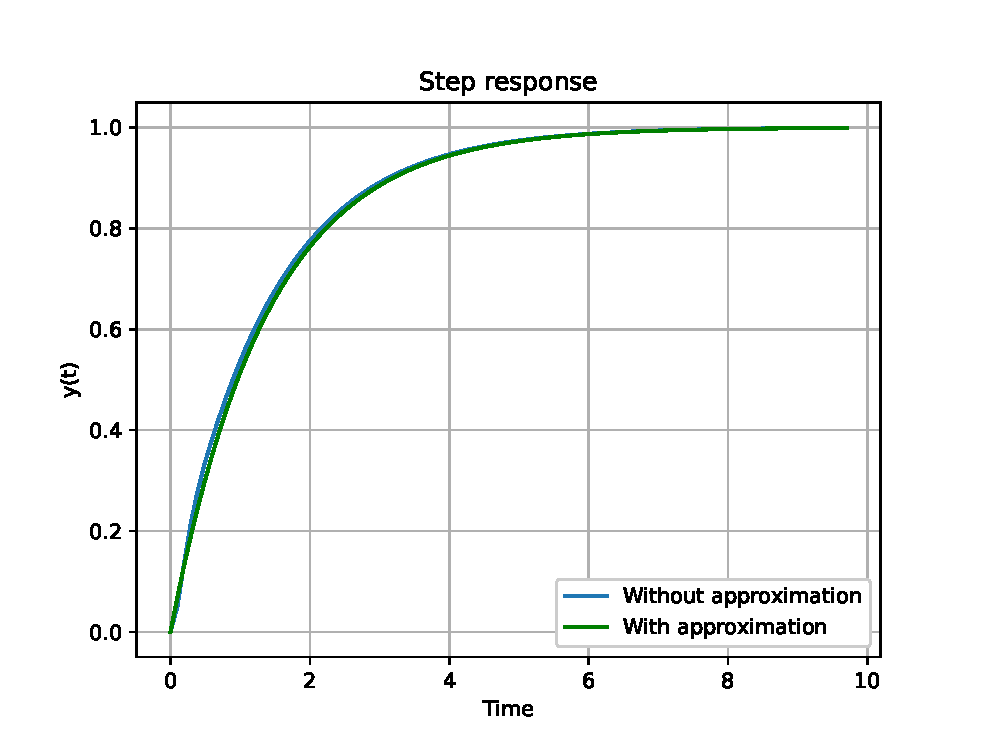
\includegraphics[width=\columnwidth]{./figs/ee18btech11047/ee18btech11047_4.eps}
\caption{}
\label{fig:ee18btech11047_4}
\end{figure}
\end{enumerate}

\caption{}
\label{table:ee18btech11047}
\end{table}
The real poles \brak{p_{1},p_{2}} and zeros \brak{z_{1},z_{2}} cancel out each other as mentioned above.So, we are left with the two conjugate poles.\\
The approximated transfer function is 
\begin{align}
T_{1}(s) &= \frac{K_{1}}{(s-p_{3})(s-p_{4})}\\ 
T(0) &= T_{1}(0)\\
\implies K_{1} &= p_{3}p_{4}\\
T_{1}(s) &= \frac{47.09}{s^{2}+3.74s+47.09}
\end{align}
\item Estimate the transient response of the obtained second order system using the respective bode plot.\\
\solution The following code generates the bode plot for open loop transfer function.
\begin{lstlisting}
codes/ee18btech11047/ee18btech11047_2.py
\end{lstlisting}
\begin{figure}[!ht]
\centering
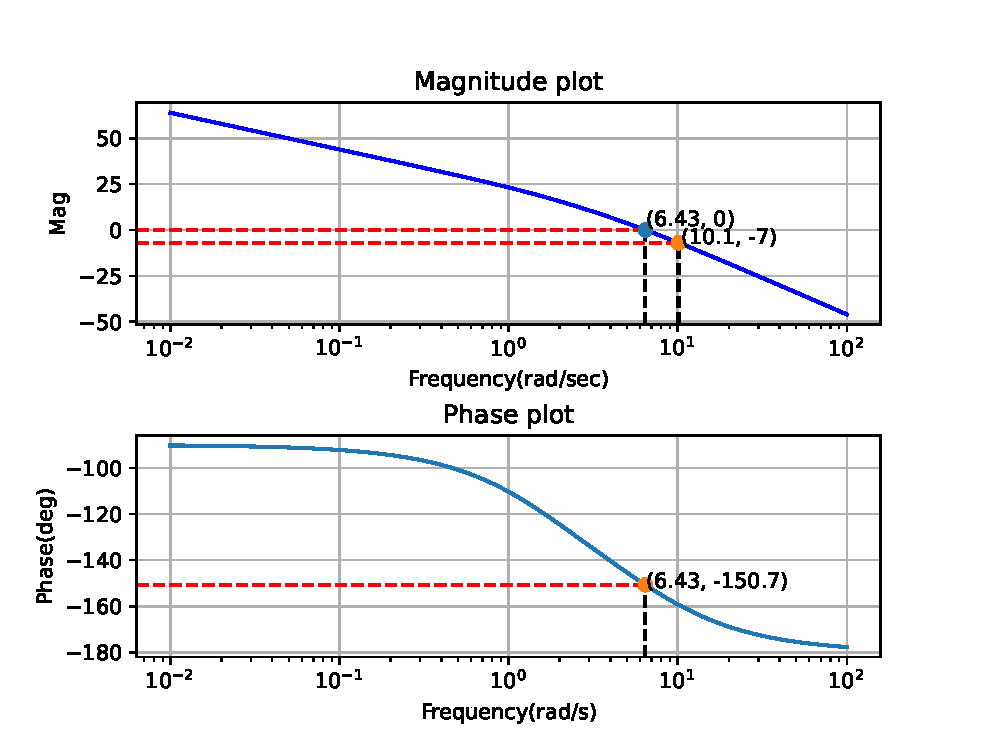
\includegraphics[width=\columnwidth]{./figs/ee18btech11047/ee18btech11047_2.eps}
\caption{1}
\label{fig:ee18btech11047_2}
\end{figure}
The phase margin is 
\begin{align}
\phi_{M} &= 180\degree-150.7\degree \implies \phi_{M} = 29.3\degree \label{eq:ee18btech11047_ph}
\end{align}
The closed-loop bandwith, $\omega_{BW}$(-3 dB frequency), equals the frequency at which the open-loop magnitude response is around -7 dB.
\begin{align}
\omega_{BW} = 10.1  rad/sec \label{eq:ee18btech11047_bw}
\end{align}
\textbf{Damping ratio:} \\
Substitute $\phi_{M}$ value from equation(\ref{eq:ee18btech11047_ph})
\begin{align}
\phi_{M} &= {tan}^{-1}\brak{\frac{2\zeta}{\sqrt{-2\zeta^{2}+\sqrt{1+4\zeta^{2}}}}}\\
\implies \zeta &= 0.34
\end{align}
\textbf{Settling time:} \\
Substitute $\omega_{BW}$ value from equation(\ref{eq:ee18btech11047_bw}) and $\zeta$
\begin{align}
T_{s}&= \frac{4}{\omega_{BW}\zeta}\sqrt{(1-2\zeta^2)+\sqrt{4\zeta^4-4\zeta^2+2}}\\
\implies T_{s} &= 1.65 sec   \\
\end{align}
\textbf{Peak time:}
\begin{align}
T_{p} &= \frac{\pi\zeta T_{s}}{4\sqrt{1-\zeta^2}}\\
\implies T_{p} &= 0.325 sec
\end{align}
\textbf{Percent overshoot:}
\begin{align}
\% OS&=100e^{-(\frac{\zeta\pi}{\sqrt{1-\zeta^2}})}\\
\implies \% OS &= 35.1 \%
\end{align}
Note that the answers will be approximate due to the dominant pole approximation.\\
The following code generates the step response of the system.
\begin{lstlisting}
codes/ee18btech11047/ee18btech11047_3.py
\end{lstlisting}
\begin{figure}[!ht]
\centering
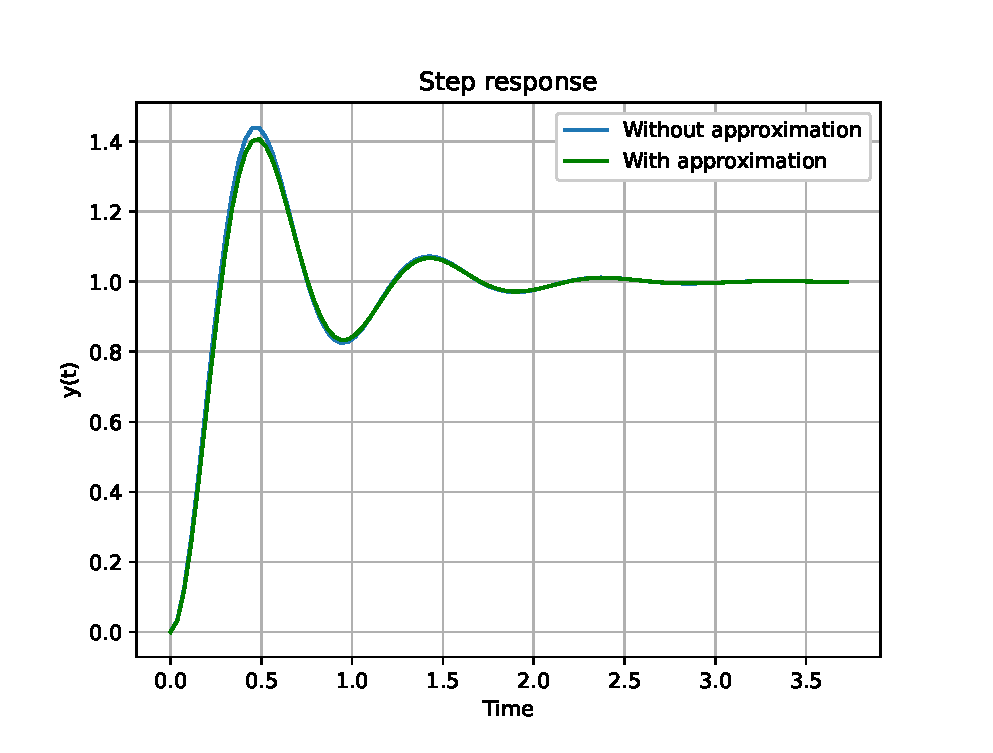
\includegraphics[width=\columnwidth]{./figs/ee18btech11047/ee18btech11047_3.eps}
\caption{2}
\label{fig:ee18btech11047_3}
\end{figure}
\item Find the approximate transfer function for the open loop transfer function
\begin{align}
G(s) &= \frac{75(1+0.2s)}{s(s^{2}+16s+100)}
\end{align}
\solution Using equation \eqref{eq:ee18btech11047_ctf}
\begin{align}
T(s) = \frac{75(1+0.2s)}{s^3 + 16s^2 + 115s +75} 
\end{align}
The following code gives the poles and zeros of the transfer function.
\begin{lstlisting}
codes/ee18btech11047/ee18btech11047_4.py
\end{lstlisting}
\begin{table}[!ht]
\centering
\tikzstyle{block} = [draw, fill=blue!20, rectangle, 
    minimum height=3em, minimum width=6em]
\tikzstyle{sum} = [draw, fill=blue!20, circle, node distance=1cm]
\tikzstyle{input} = [coordinate]
\tikzstyle{output} = [coordinate]
\tikzstyle{pinstyle} = [pin edge={to-,thin,black}]

\begin{tikzpicture}[auto, node distance=2cm,>=latex']
    \node [input, name=input] {};
    \node [sum, right of=input] (sum) {};
    \node [block, right of=sum] (controller) {$G$};
    \node [output, right of=controller] (output) {};
    \node [block, below of=controller] (feedback) {$H$};
    \draw [draw,->] (input) -- node {} (sum);
    \draw [->] (sum) -- node {$V_i$} (controller);
    \draw [->] (controller) -- node [name=y] {$V_o$}(output);
    \draw [->] (y) |- (feedback);
    \draw [->] (feedback) -| node[pos=0.99]{$+$}  node [near end] {$V_f$} (sum);
\end{tikzpicture}

\caption{}
\label{table:ee18btech11047_2}
\end{table}
The real part of the complex conjugate poles is comparable with the zero $z_{1}$ of the transfer function.So,they cancel out each other.
The approximated transfer function is of first order.
\begin{align}
T_{2}(s) &= \frac{K_{2}}{(s-p_{1})}\\
T(0) &= T_{2}(s)\\
\implies K_{2} &= p_{1} \\
T_{2}(s) &= \frac{0.72}{s+0.72}
\end{align}
\item Estimate the transient response of the obtained first order system.\\
\solution\\
\textbf{Time constant:}\\
The time constant is the time taken by the step response to rise to 63\% of it's final value.
\begin{align}
T &= \frac{1}{|pole|}\\
T &= \frac{1}{0.72} = 1.388 sec
\end{align}
\textbf{Rise time:}\\
Rise time is the time for the waveform to go from 0.1 to 0.9 of it's final value.
\begin{align}
T_{r} &= \frac{2.2}{|pole|}\\
T_{r} &= \frac{2.2}{0.72} = 3.05 sec
\end{align}
\textbf{Settling time:}\\
Settling time is defined as the time for the response to reach and stay within, 2\% of its final value.
\begin{align}
T_{s} &= \frac{4}{|pole|}\\
T_{s} &= \frac{4}{0.72}=5.55 sec
\end{align}
The following code plots the step response of the system.
\begin{lstlisting}
codes/ee18btech11047/ee18btech11047_5.py
\end{lstlisting}
\begin{figure}[!ht]
\centering
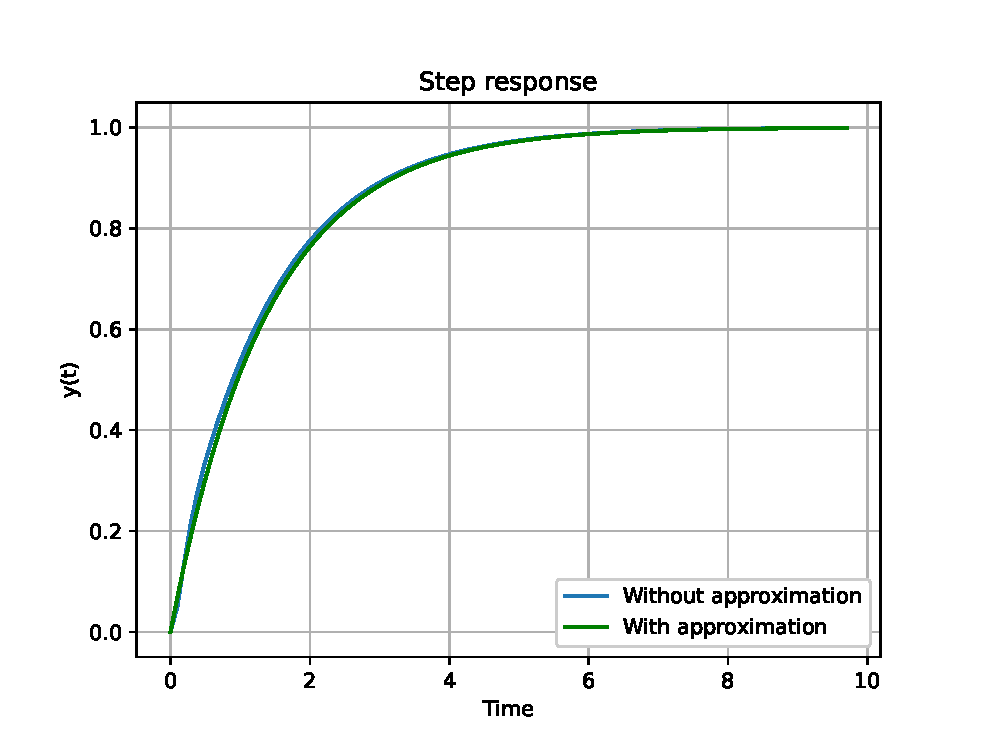
\includegraphics[width=\columnwidth]{./figs/ee18btech11047/ee18btech11047_4.eps}
\caption{}
\label{fig:ee18btech11047_4}
\end{figure}
\end{enumerate}

\caption{}
\label{table:ee18btech11047}
\end{table}
The real poles \brak{p_{1},p_{2}} and zeros \brak{z_{1},z_{2}} cancel out each other as mentioned above.So, we are left with the two conjugate poles.\\
The approximated transfer function is 
\begin{align}
T_{1}(s) &= \frac{K_{1}}{(s-p_{3})(s-p_{4})}\\ 
T(0) &= T_{1}(0)\\
\implies K_{1} &= p_{3}p_{4}\\
T_{1}(s) &= \frac{47.09}{(s+1.87-6.60j)(s+1.87+6.60j)} \label{eq:ee18btech11047_a_tf1}
\end{align}
\item Estimate the transient response of the obtained second order system using bode plot.\\
\solution The following code generates the bode plot for open loop transfer function.
\begin{lstlisting}
codes/ee18btech11047/ee18btech11047_2.py
\end{lstlisting}
\begin{figure}[!ht]
\centering
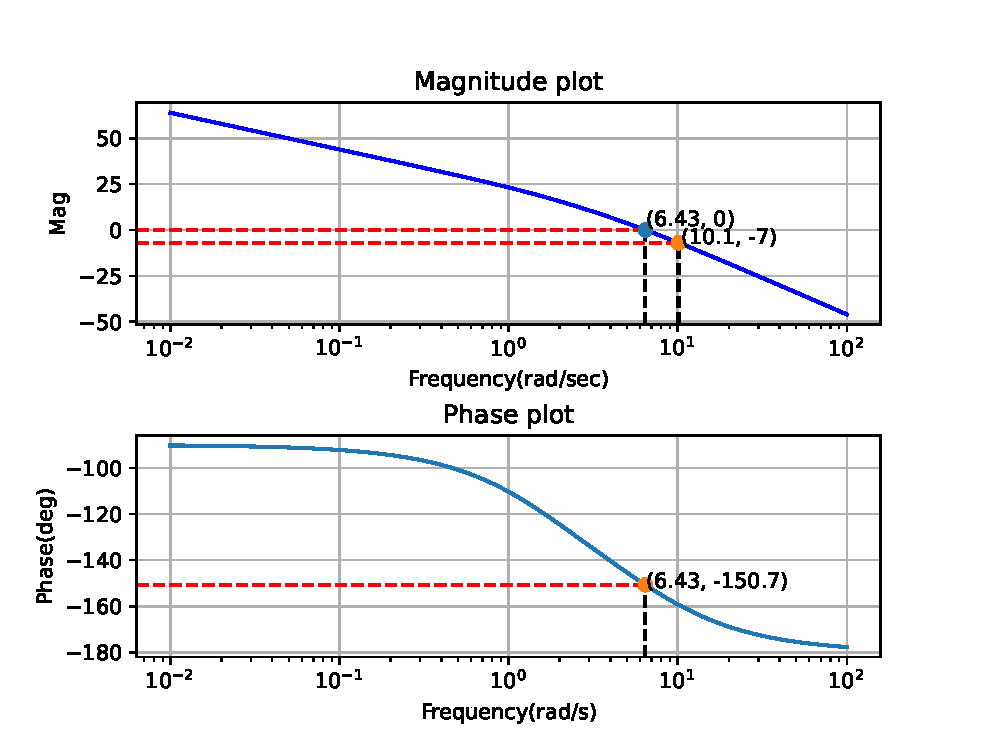
\includegraphics[width=\columnwidth]{./figs/ee18btech11047/ee18btech11047_2.eps}
\caption{}
\label{fig:ee18btech11047_2}
\end{figure}

The phase margin is 
\begin{align}
\phi_{M} &= 180\degree-150.7\degree \implies \phi_{M} = 29.3\degree \label{eq:ee18btech11047_ph}
\end{align}
The closed-loop bandwith, $\omega_{BW}$(-3 dB frequency), equals the frequency at which the open-loop magnitude ressponse is around -7 dB.
\begin{align}
\omega_{BW} = 10.1  rad/sec \label{eq:ee18btech11047_bw}
\end{align}
\item \textbf{Damping ratio} \\
Substitute $\phi_{M}$ value from equation(\ref{eq:ee18btech11047_ph})
\begin{align}
\phi_{M} &= \inv{tan}^{-1}\brak{\frac{2\zeta}{\sqrt{-2\zeta^{2}+\sqrt{1+4\zeta^{2}}}}}\\
\implies \zeta &= 0.34
\end{align}
\item \textbf{Settling time} \\
Substitute $\omega_{BW}$ value from equation(\ref{eq:ee18btech11047_bw}) and $\zeta$
\begin{align}
T_{s}&= \frac{4}{\omega_{BW}\zeta}\sqrt{(1-2\zeta^2)+\sqrt{4\zeta^4-4\zeta^2+2}}\\
\implies T_{s} &= 1.65 sec   
\end{align}
\item \textbf{Peak time} \\
\begin{align}
T_{p} &= \frac{\pi\zeta T_{s}}{4\sqrt{1-\zeta^2}}\\
\implies T_{p} &= 0.325 sec
\end{align}
\item \textbf{Percent overshoot}
\begin{align}
\% OS&=100e^{-(\frac{\zeta\pi}{\sqrt{1-\zeta^2}})}\\
\implies \% OS &= 35.1 \%
\end{align}
Note that the answers will be approximate due to the dominant pole approximation.\\
The following code generates the step response of the system.
\begin{lstlisting}
codes/ee18btech11047/ee18btech11047_3.py
\end{lstlisting}
\begin{figure}[!ht]
\centering
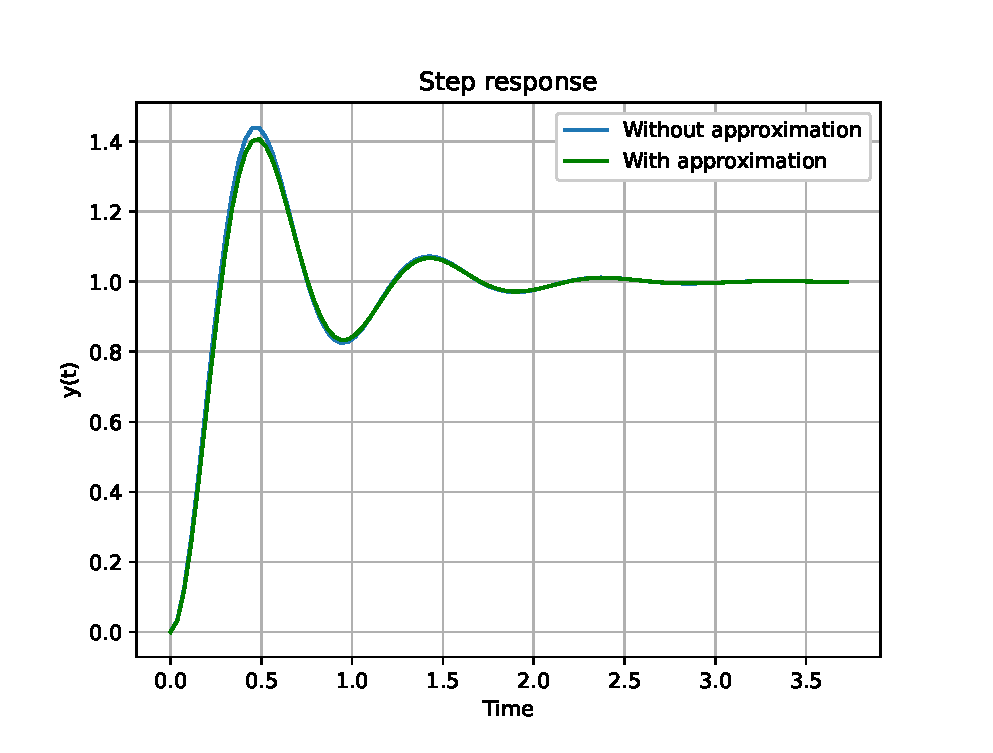
\includegraphics[width=\columnwidth]{./figs/ee18btech11047/ee18btech11047_3.eps}
\caption{}
\label{fig:ee18btech11047_3}
\end{figure}
\item Find the approximate transfer function for the open loop transfer function
\begin{align}
G(s) &= \frac{75(1+0.2s)}{s(s^{2}+16s+100)}
\end{align}
\solution Using equation(\ref{eq:ee18btech11047_tf})
\begin{align}
T(s) = \frac{75(1+0.2s)}{s^3 + 16s^2 + 115s +75} 
\end{align}
The following code gives the poles and zeros of the transfer function.
\begin{lstlisting}
codes/ee18btech11047/ee18btech11047_4.py
\end{lstlisting}
\begin{table}[!ht]
\centering
\tikzstyle{block} = [draw, fill=blue!20, rectangle, 
    minimum height=3em, minimum width=6em]
\tikzstyle{sum} = [draw, fill=blue!20, circle, node distance=1cm]
\tikzstyle{input} = [coordinate]
\tikzstyle{output} = [coordinate]
\tikzstyle{pinstyle} = [pin edge={to-,thin,black}]

\begin{tikzpicture}[auto, node distance=2cm,>=latex']
    \node [input, name=input] {};
    \node [sum, right of=input] (sum) {};
    \node [block, right of=sum] (controller) {$G$};
    \node [output, right of=controller] (output) {};
    \node [block, below of=controller] (feedback) {$H$};
    \draw [draw,->] (input) -- node {} (sum);
    \draw [->] (sum) -- node {$V_i$} (controller);
    \draw [->] (controller) -- node [name=y] {$V_o$}(output);
    \draw [->] (y) |- (feedback);
    \draw [->] (feedback) -| node[pos=0.99]{$+$}  node [near end] {$V_f$} (sum);
\end{tikzpicture}

\caption{}
\label{table:ee18btech11047_2}
\end{table}
The real part of the complex conjuagte poles is comparable with the zero z1 of the transfer function.So,they cancel out each other.
The approximated transfer function is of first order.
\begin{align}
T_{2}(s) &= \frac{K_{2}}{(s-p_{1})}\\
T(0) &= T_{2}(s)\\
\implies K_{2} &= p_{1} \\
T_{2}(s) &= \frac{0.72}{s+0.72} \label{eq:ee18btech11047_a_tf2}
\end{align}

\item Estimate the transient response of the obtained first order system.\\
\item \textbf{Time constant}\\
The time constant is the time taken by the step response to rise to 63\% of it's final value.
\begin{align}
T &= \frac{1}{|pole|}\\
T &= \frac{1}{0.72} = 1.388 sec
\end{align}
\item \textbf{Rise time}\\
Rise time is the time for the waveform to go from 0.1 to 0.9 of it's final value.
\begin{align}
T_{r} &= \frac{2.2}{|pole|}\\
T_{r} &= \frac{2.2}{0.72} = 3.05 sec
\end{align}
\item \textbf{Settling time}\\
Settling time is defined as the time for the response to reach ,and stay within, 2\% of its final value.
\begin{align}
T_{s} &= \frac{4}{|pole|}\\
T_{s} &= \frac{4}{0.72}=5.55 sec
\end{align}
The following code plots the step response of the system.
\begin{lstlisting}
codes/ee18btech11047/ee18btech11047_5.py
\end{lstlisting}
\begin{figure}[!ht]
\centering
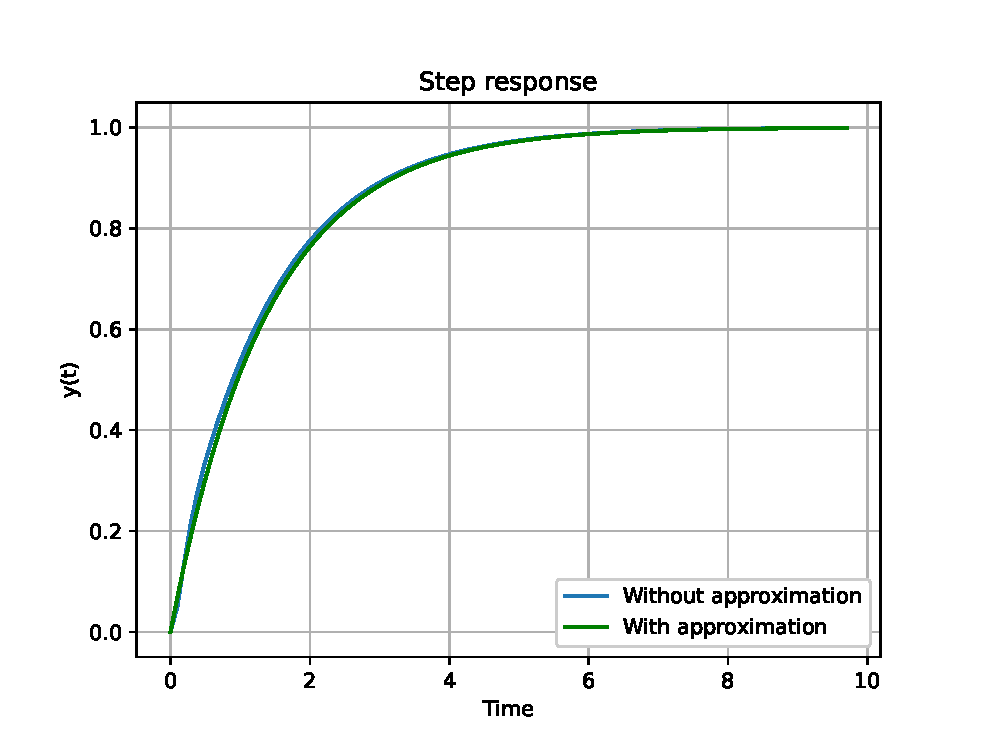
\includegraphics[width=\columnwidth]{./figs/ee18btech11047/ee18btech11047_4.eps}
\caption{}
\label{fig:ee18btech11047_4}
\end{figure}
\end{enumerate}
